%This chapter present and discuss the research results, respectively.
%They are often usefully combined into one section, however, because readers can seldom make sense of results alone without accompanying interpretation.
%They need to be told what the results mean.



\chapter{Results and Discussion}\label{chapter:results}
	In this chapter, we use our custom simulation test-bed to assess the models we presented in both synchronous and asynchronous cases.   In Section \ref{section:asynchronousModel}, we evaluate the accuracy of these models.   We also give an experimental evaluation of the gain brought by our solutions on the considered pattern.\\
	In Section \ref{section:experimentalCase}, we compare the performances of our \notationaio\space solution using both our \toolSimulationSoftware\space and our custom implementation of the \toolTargetSoftware.   We show how our solution might interfere with a real-life application (namely: the \toolTargetSoftware software).   We show how we identified the causes of these different perturbations.   We also evaluate the sequence of custom solutions that lighten such perturbations.\\


%--------------------------------------------
\section{Asynchronous model and improvements} \label{section:asynchronousModel}
	\subsection{First model assessment (single \notationIO\space device)}\label{subsection:AIO_firstApproachAssessment}
		In order to assess the first theoretical model (see Section \ref{subsection:firstModel}), one should first be able to assess the \emph{write} time $W$ of each buffer.   According to the model hypotheses, this \emph{write} time is considered as constant (for a fixed data size and a given hardware platform).   Figure \ref{fig:writeTimeExample} shows the experimental evaluation that we have obtained on the two considered platforms.\\

			\begin{figure*}[!h]
				\centering
				\begin{subfigure}[b]{0.475\textwidth}
					\centering
					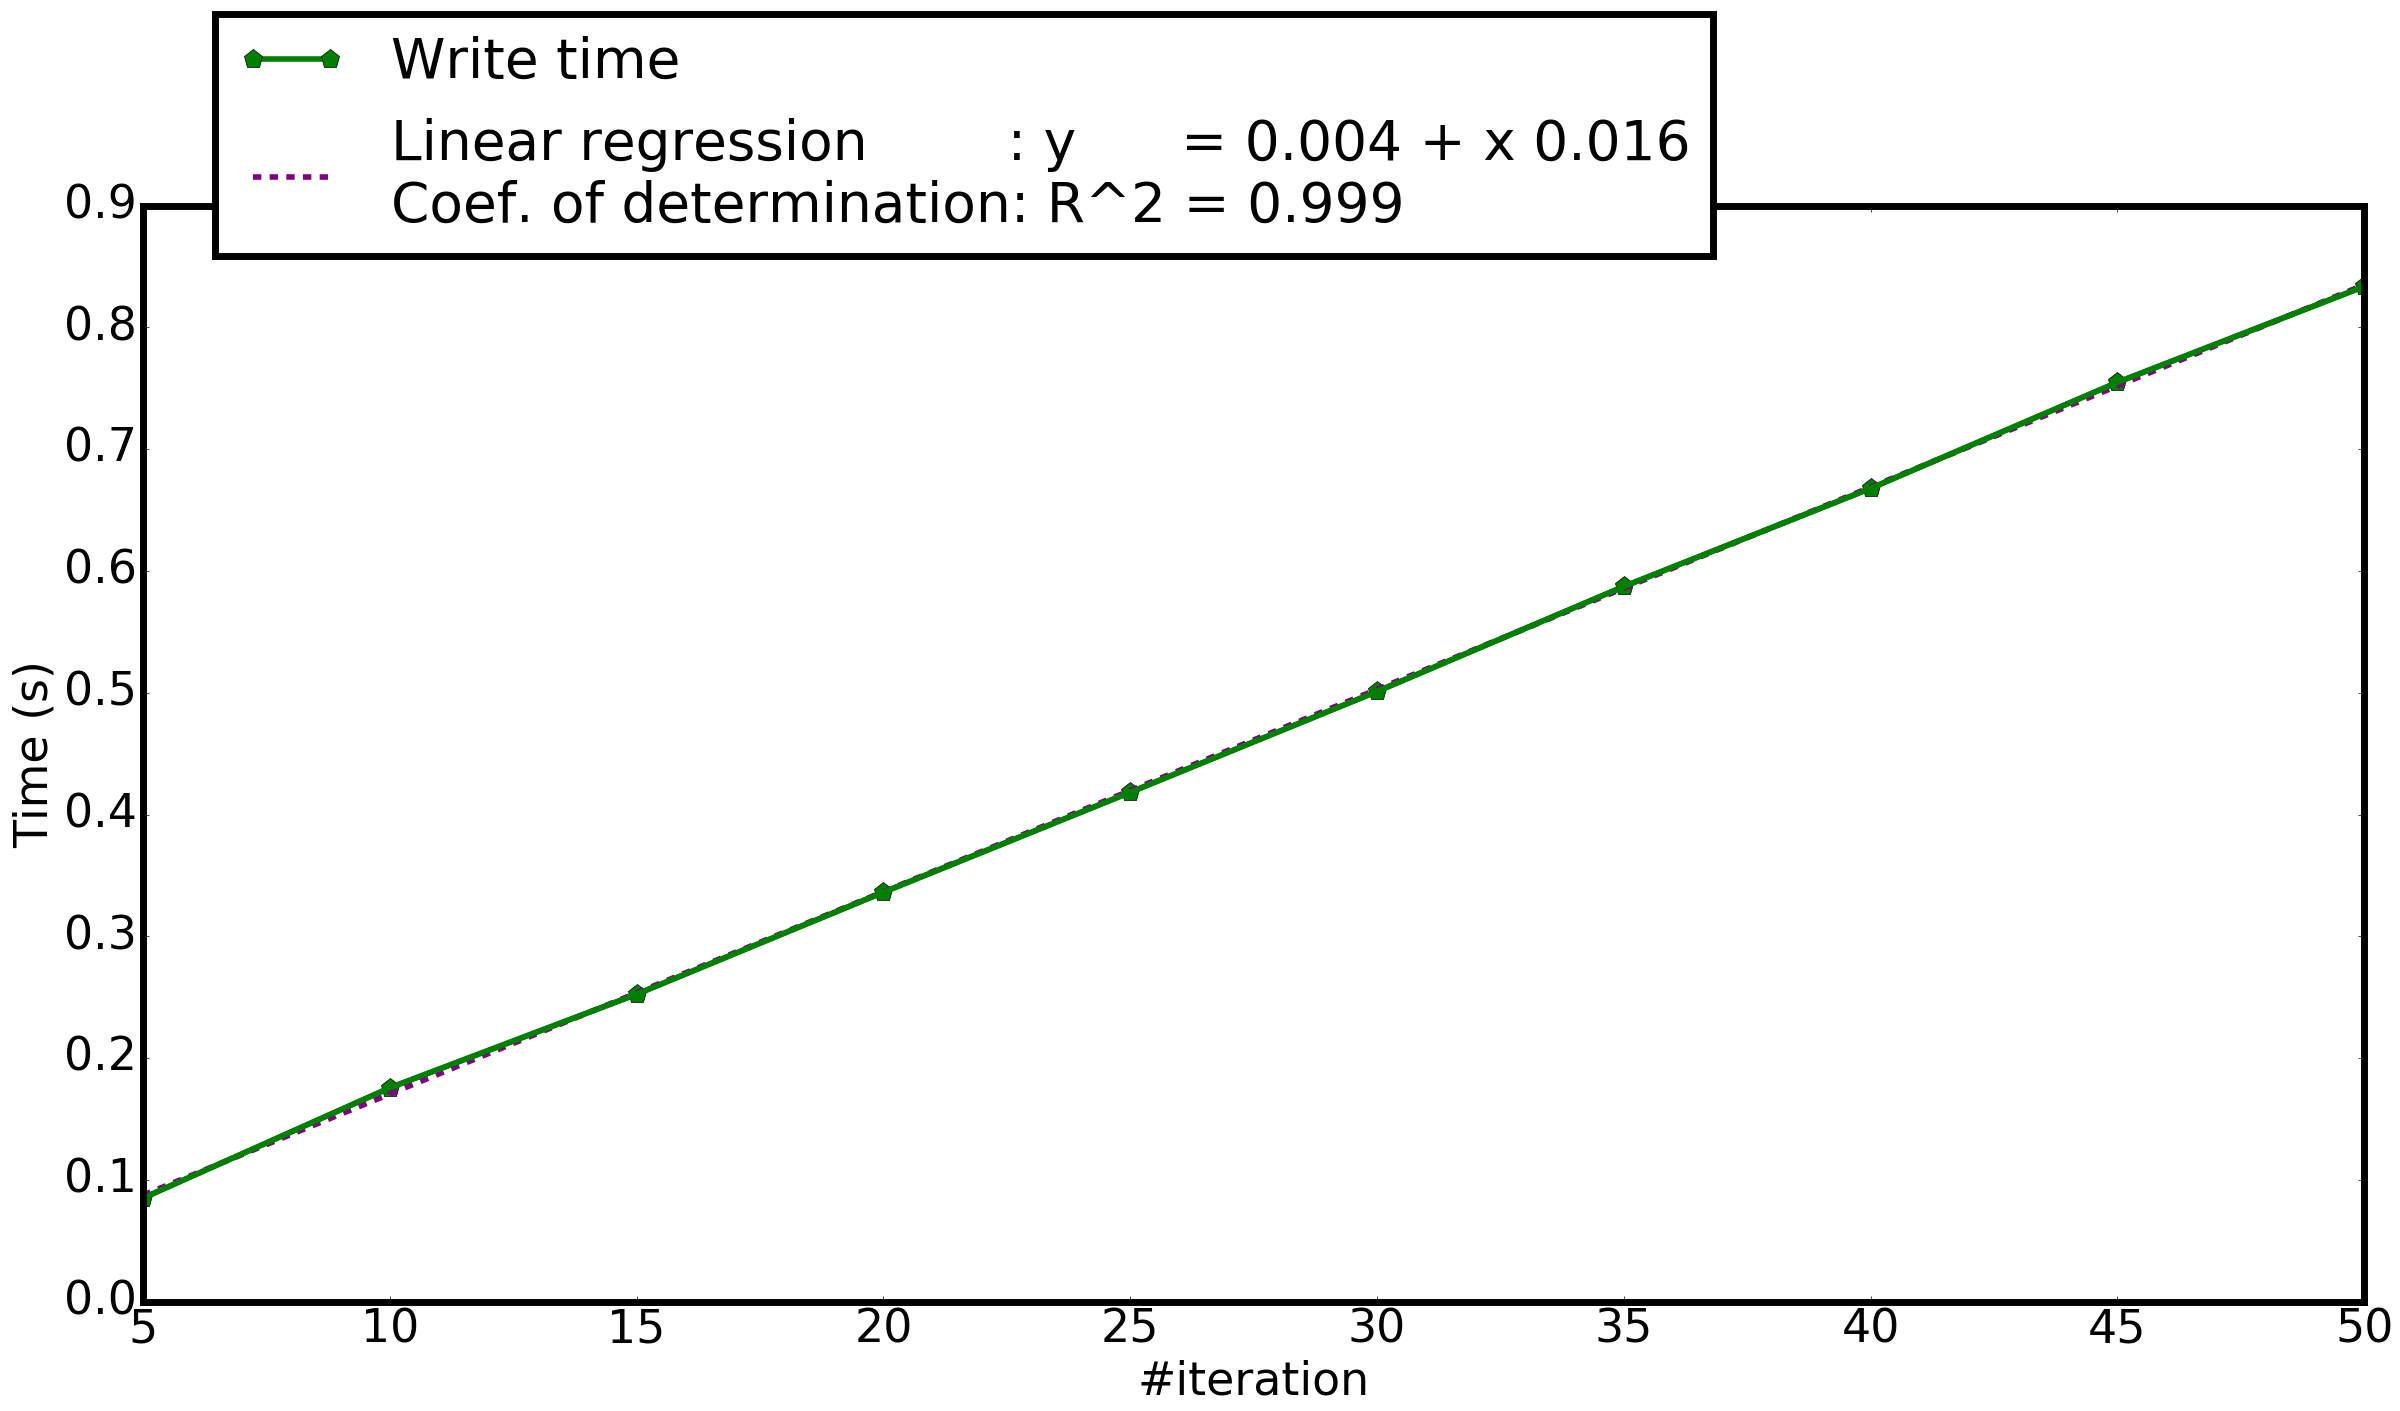
\includegraphics[width=\textwidth]{charts/writeTimeExample_workstation_8core.png}
					\caption[\targetPlatformLaptop \space @ \targetPlatformLaptopFrequency]
					{{\small \targetPlatformLaptop \space @ \targetPlatformLaptopFrequency}}
					\label{fig:writeTimeExample_workstation}
				\end{subfigure}
				\hfill
				\begin{subfigure}[b]{0.475\textwidth}  
					\centering 
					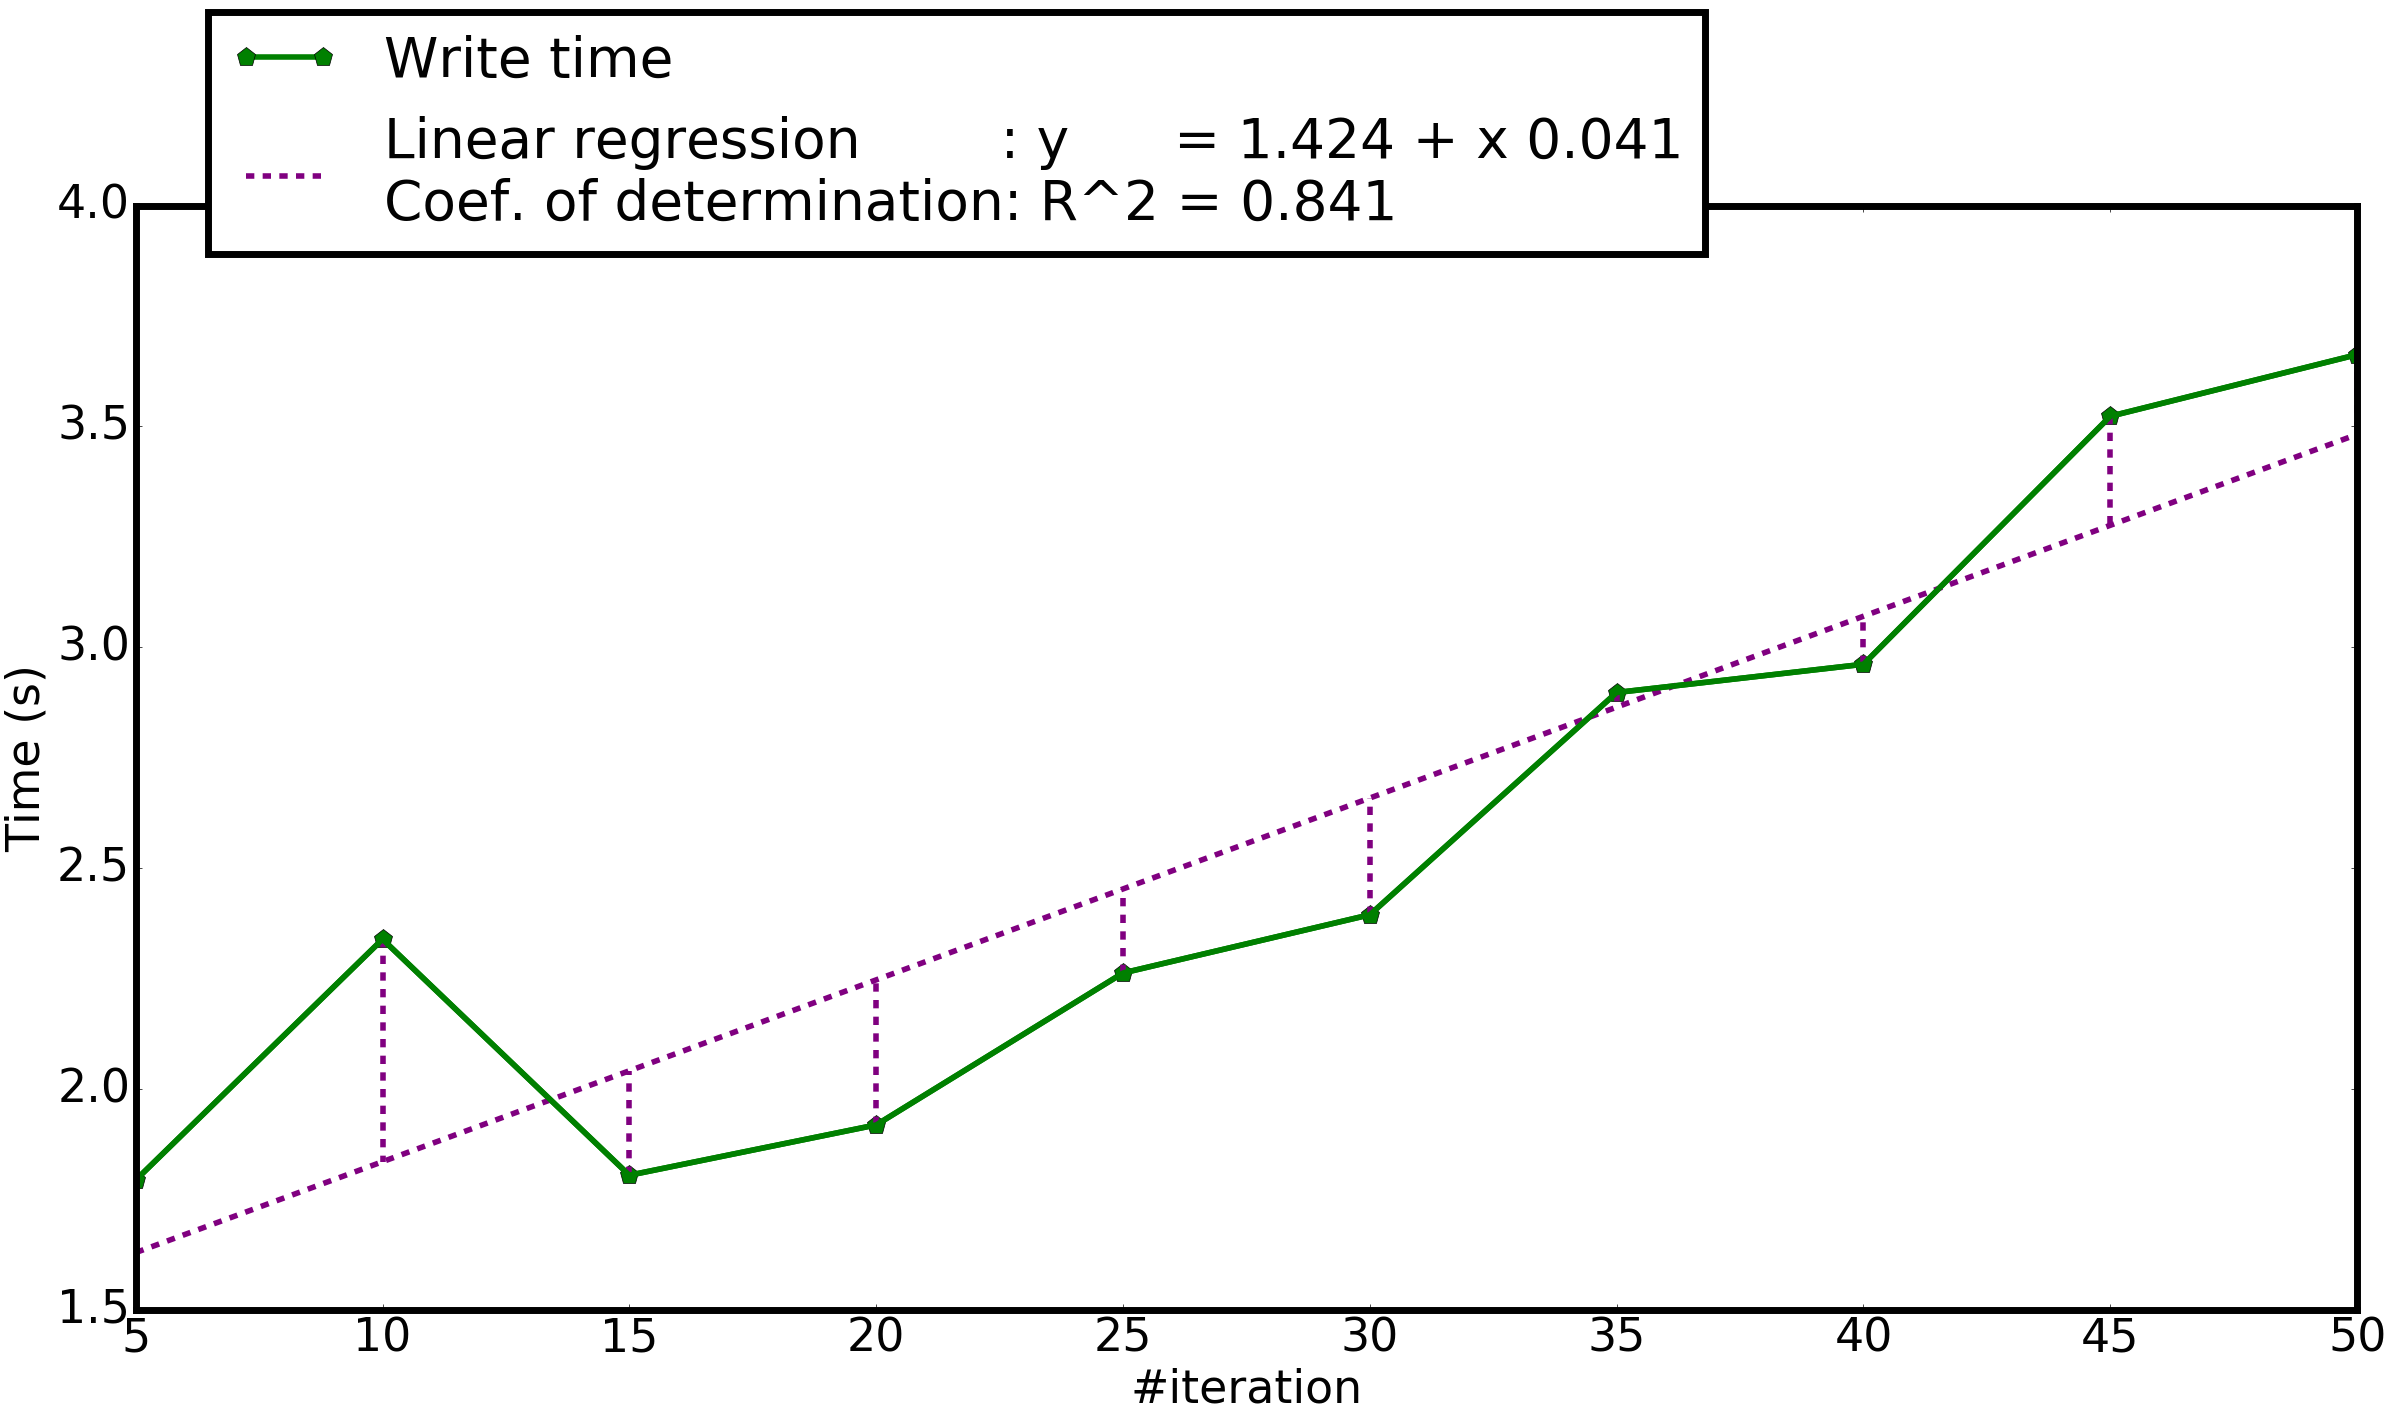
\includegraphics[width=\textwidth]{charts/writeTimeExample_HPC_jureca.png}
					\caption[]%
					{{\small \targetPlatformHpc \space @ \targetPlatformHpcFrequency}}    
					\label{fig:writeTimeExample_hpc}
				\end{subfigure}
				\caption{Experimental assessment of the time for writing 50,000,000 bytes}
				\label{fig:writeTimeExample}
			\end{figure*}

		One could notice on these experimental results that the assessed \emph{write} time is roughly constant through different assessments (excluding the outliers which are regularly observed at the beginning of each experimentation on the HPC platform\footnote{This outlier corresponds probably to a warm-up phase before the pre-loader of the \notationIO\space device becomes fully efficient (for the currently accessed \notationIO\space pattern)}).   Indeed, the value of the \emph{write} time $W$ fluctuates within a range of $10 ^{-2}$ seconds (for both considered hardware platforms).   As the measured computation times ($C$) fluctuates within a higher range of $10^{-1}$ seconds (see Section \ref{section:experimentalCase}), then the variation of $W$ could be considered as comparatively negligible.   The retained \emph{write} time approximation is the slope of the linear regression on Figure \ref{fig:writeTimeExample}.   This value (for writing $50,000,000$ bytes) is $W=0.016$ seconds for the \targetPlatformLaptop\space (Figure \ref{fig:writeTimeExample_workstation}) and $W=0.041$ seconds for the \targetPlatformHpc\space (Figure \ref{fig:writeTimeExample_hpc}).\\

		Using the simulation test-bed described in Section \ref{subsection:simulationTestbed}, we compared the asynchronous implementation with the synchronous one and the theoretical model (see Figure \ref{fig:model0_assessment}).\\
			\begin{figure*}[!h]
				\centering
				\begin{subfigure}[b]{0.475\textwidth}
					\centering
					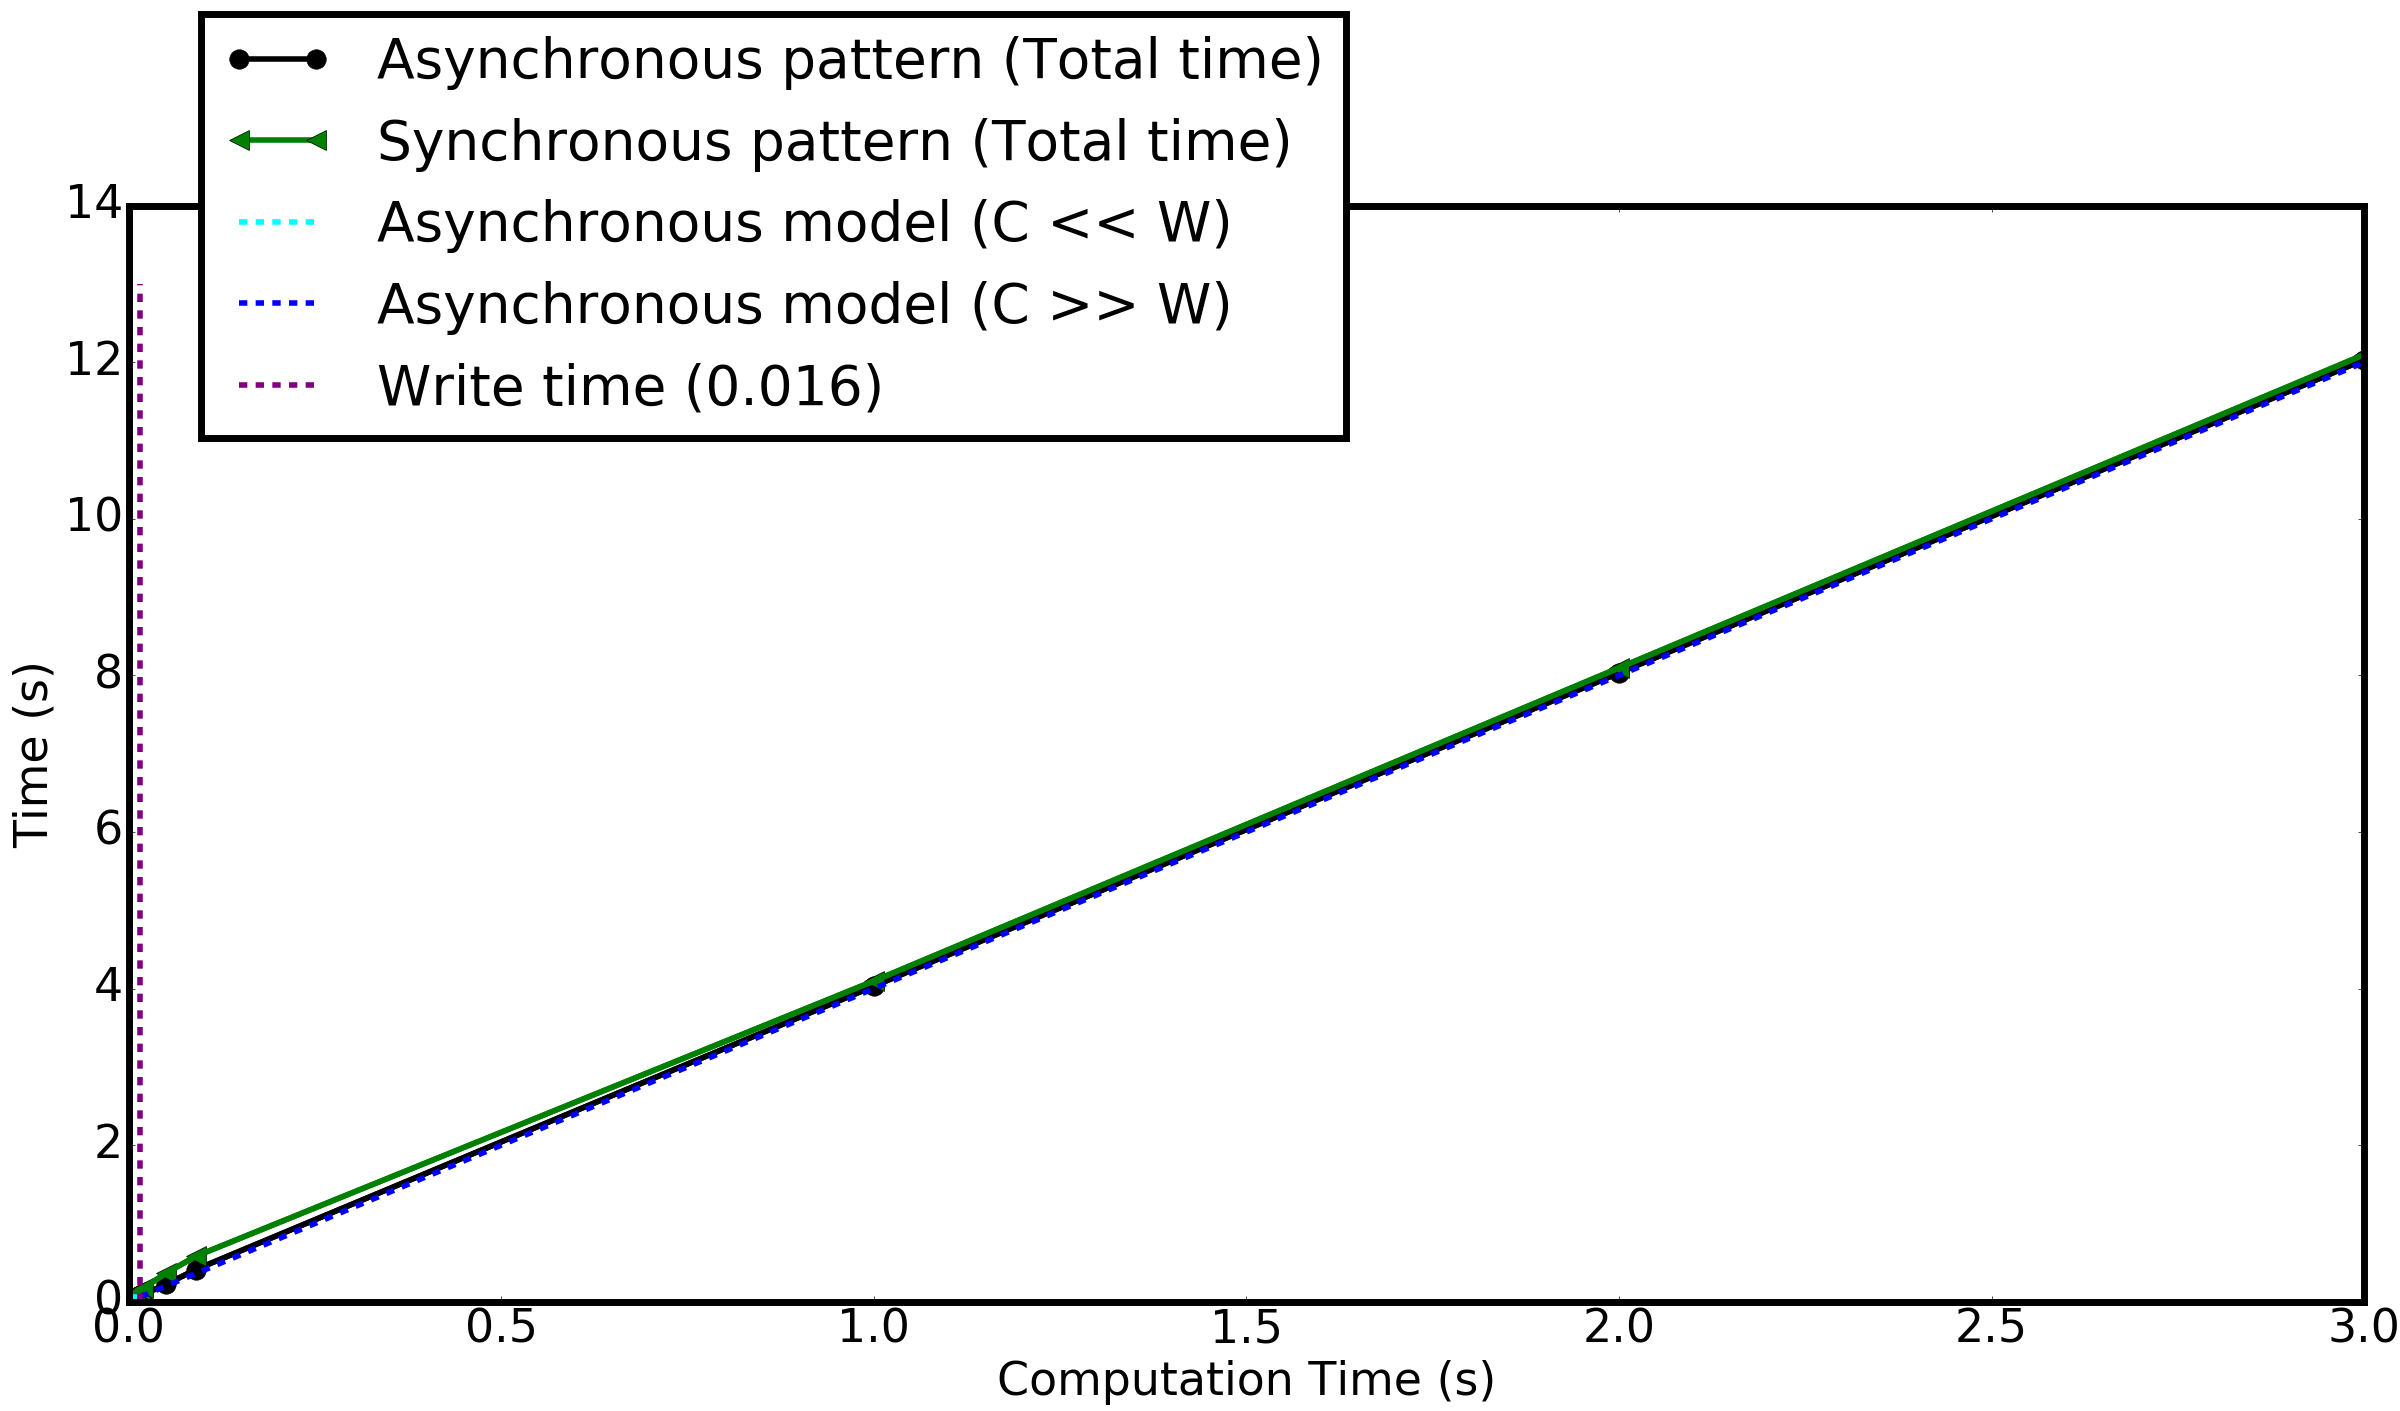
\includegraphics[width=\textwidth]{charts/model0_workstation_8core.png}
					\caption[\targetPlatformLaptop \space @ \targetPlatformLaptopFrequency\space (Linear scale)]%
					{{\small \targetPlatformLaptop \space @ \targetPlatformLaptopFrequency\space (Linear scale)}}
					\label{fig:model0_assessment_laptop}
				\end{subfigure}
				\hfill
				\begin{subfigure}[b]{0.475\textwidth}
					\centering
					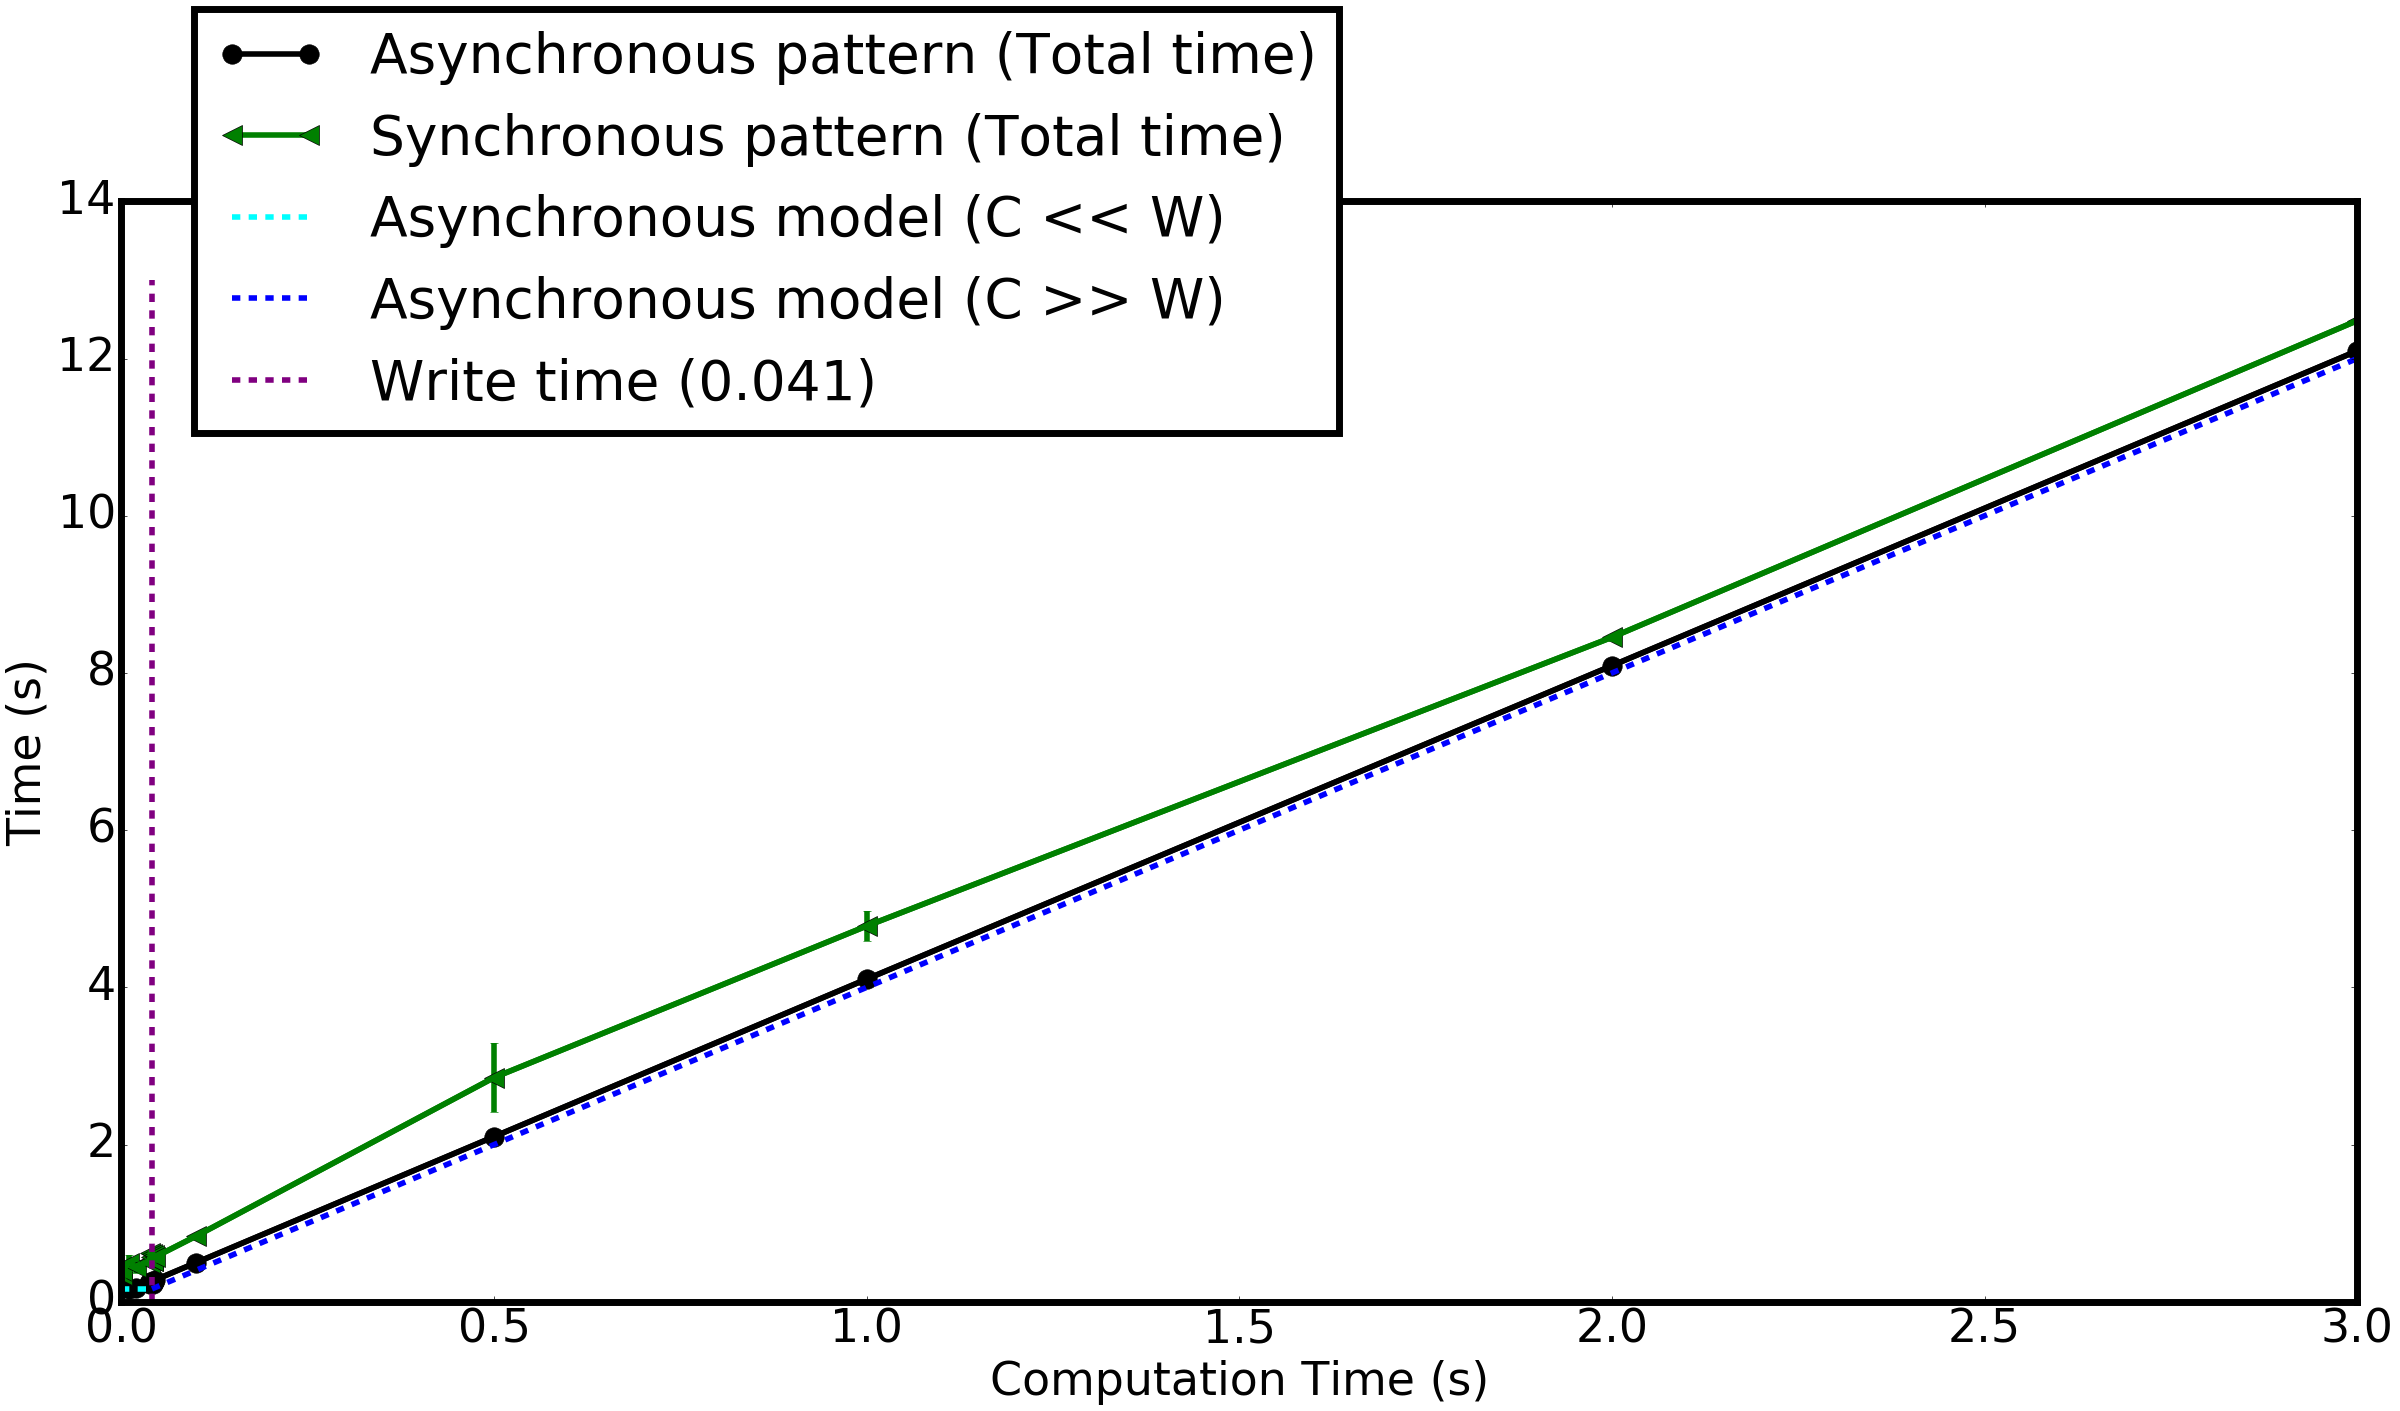
\includegraphics[width=\textwidth]{charts/model0_hpc_2Proc_1IoDevice.png}
					\caption[]%
					{{\small \targetPlatformHpc \space @ \targetPlatformHpcFrequency\space (Linear scale)}}
					\label{fig:model0_assessment_hpc}
				\end{subfigure}
				\vskip\baselineskip
				\begin{subfigure}[b]{0.475\textwidth}  
					\centering 
					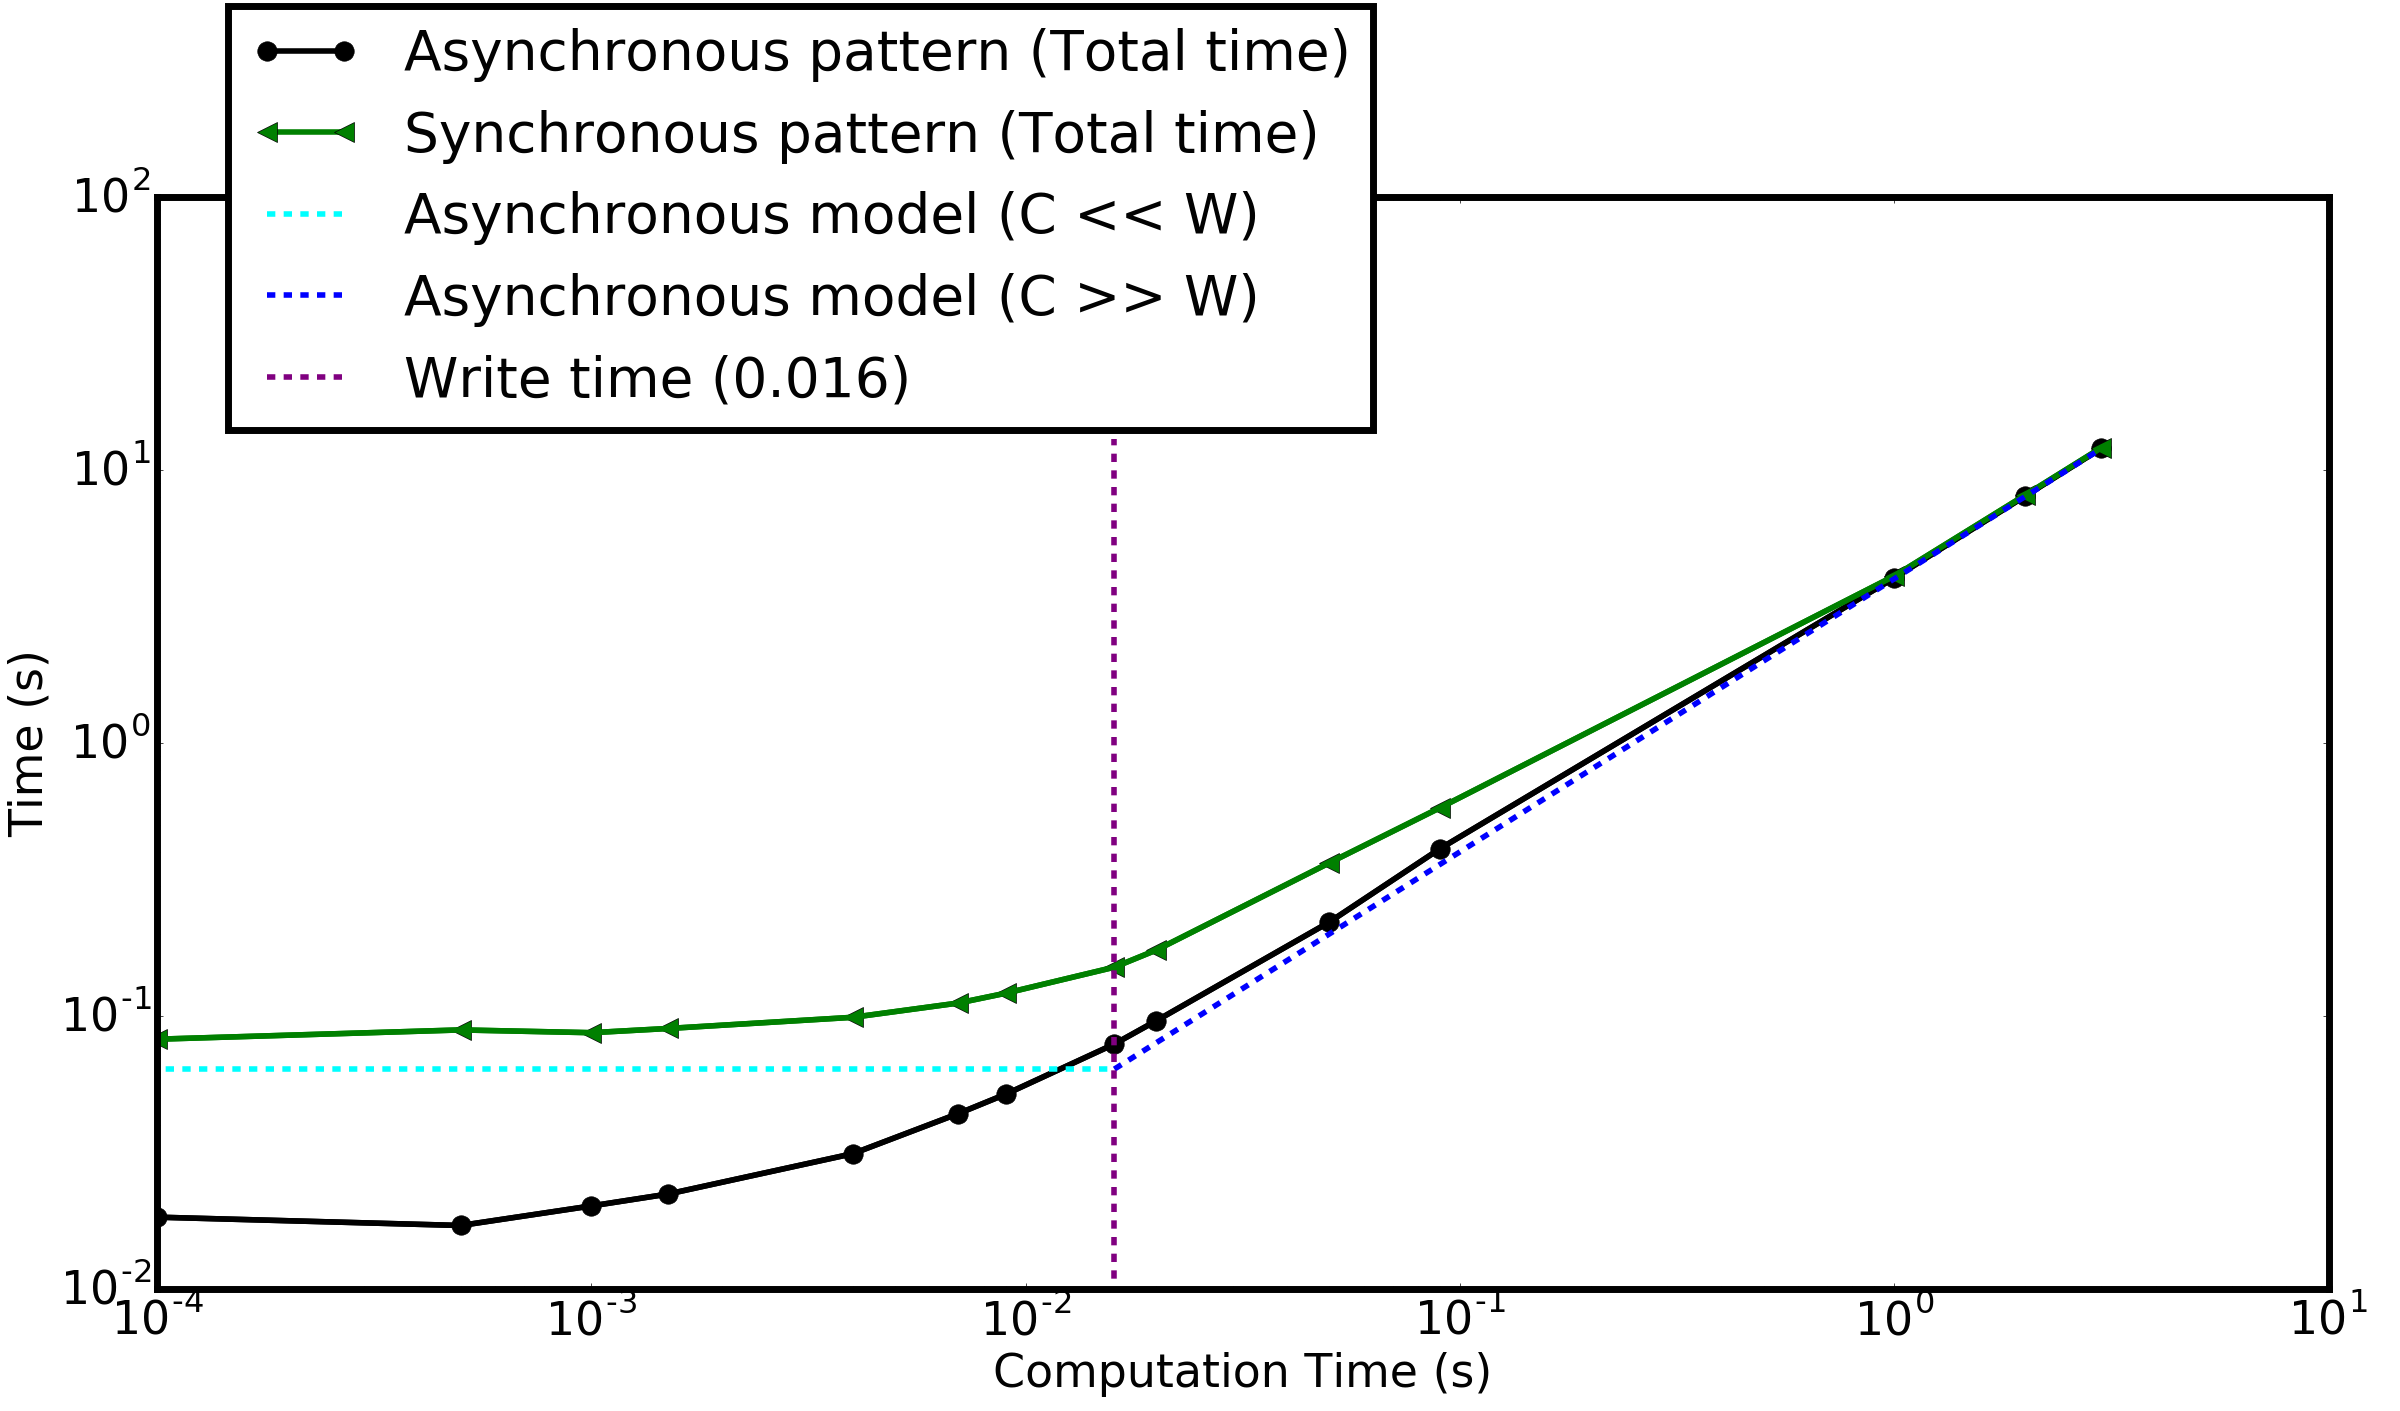
\includegraphics[width=\textwidth]{charts/model0_workstation_8core_logScale.png}
					\caption[]%
					{{\small \targetPlatformLaptop \space @ \targetPlatformLaptopFrequency\space (Log-Log scale)}}
					\label{fig:model0_assessment_laptop_log}
				\end{subfigure}
				\hfill
				\begin{subfigure}[b]{0.475\textwidth}  
					\centering 
					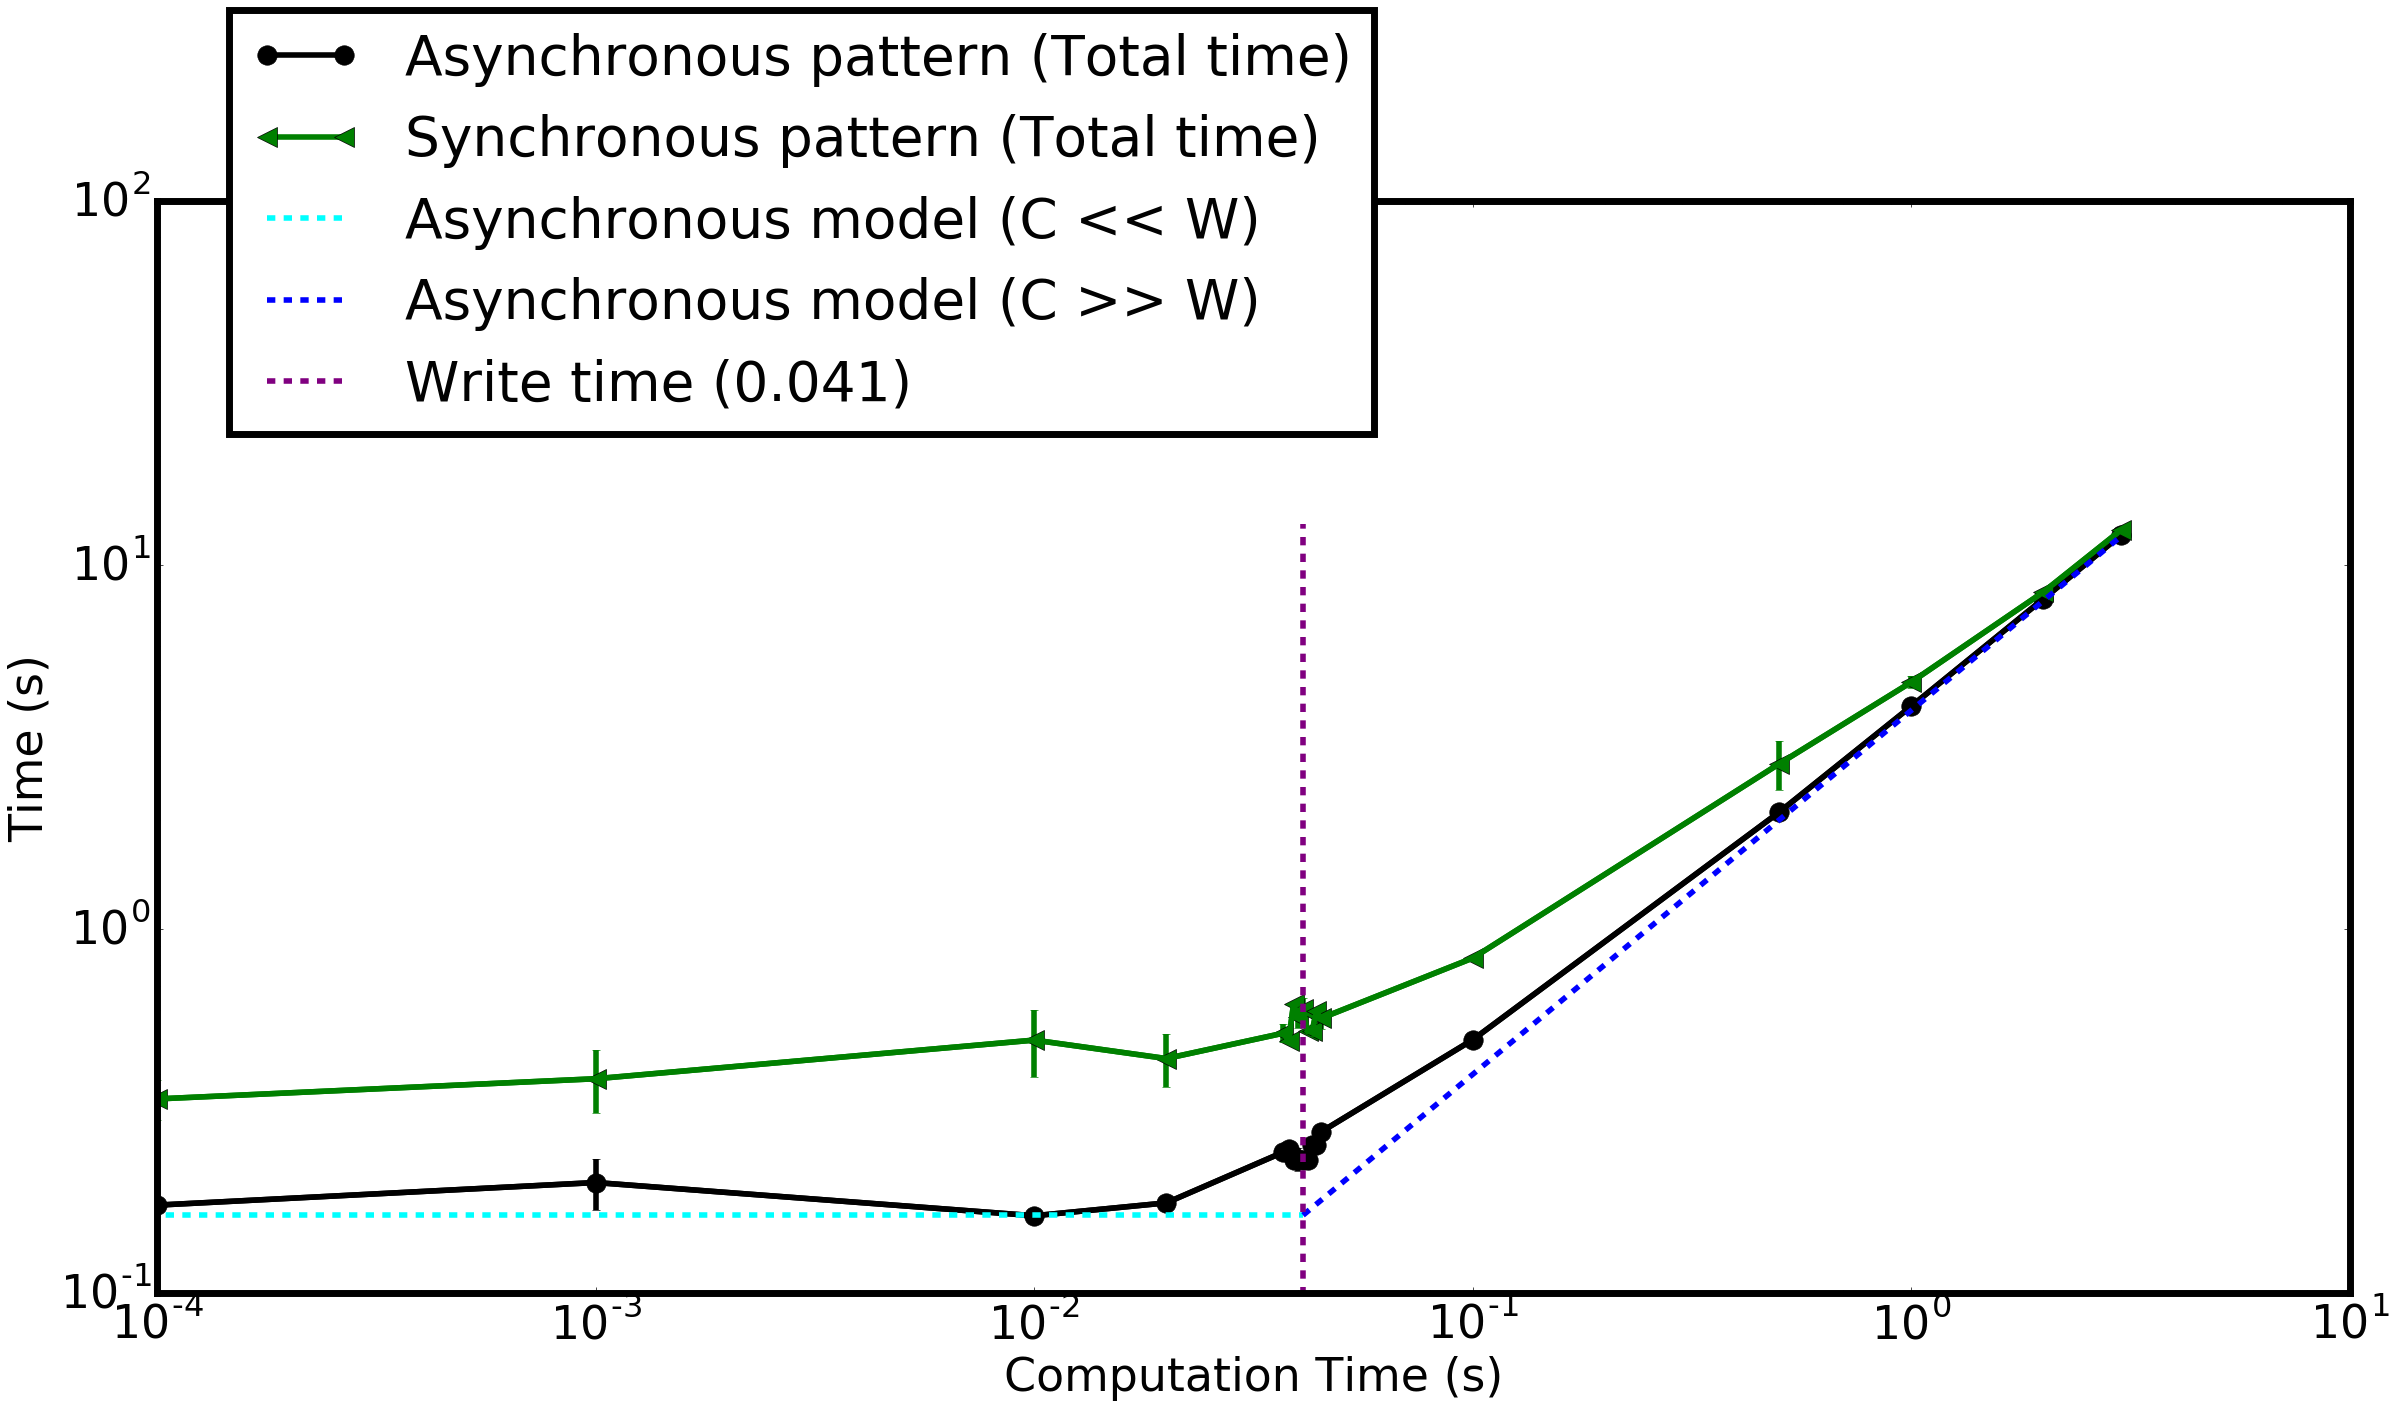
\includegraphics[width=\textwidth]{charts/model0_hpc_2Proc_1IoDevice_logScale.png}
					\caption[]%
					{{\small \targetPlatformHpc \space @ \targetPlatformHpcFrequency\space (Log-Log scale)}}
					\label{fig:model0_assessment_hpc_log}
				\end{subfigure}
				\caption{Experimental comparison of the asynchronous solution with its theoretical model and the synchronous one (50,000,000 bytes per write, 4 iterations)}
				\label{fig:model0_assessment}
			\end{figure*}

		First of all, it is clear on Figure \ref{fig:model0_assessment} that, on both targeted platforms, our custom \notationaio\space \emph{write} approach might bring a significant improvement compared to the original synchronous one.   When the computation time is in the neighbourhood of the \emph{write} time, an improvement up to $45\%$ is observed on the \targetPlatformLaptop\space and $38\%$ on the \targetPlatformHpc).   Hence, our global approach to optimize the \toolTargetSoftware\space seems comforted at this stage.\\
		Second, the trends modelled by Equations (\ref{equation:synchronousModel}) and (\ref{equation:model0}) are clearly highlighted and matched by the experimental response times of the considered pattern on Figure \ref{fig:model0_assessment}.   We can notice the accuracy in the position of the inflection point on both targeted platforms.\\

		Finally, Figure \ref{fig:model0_assessment} allows to identify the region\footnote{Set of computation times} where the improvement brought by our \notationaio\space \emph{write} algorithm is the most significant.   Indeed, we can notice on both platforms that this gain is maximal when the \emph{compute} time is in the neighbourhood of the \emph{write} time.\\

		Such a property of our \notationaio\space approach is complicated to use in a real-life software (such as the \toolTargetSoftware).   As a matter of fact, it is not easy to adapt the \emph{compute} function and make its execution time match a given value.   Furthermore, this targeted value of the \emph{compute} time is totally dependent on the host hardware platform.\\
		However, this property might be used to analyse the performance of the considered software (once shipped with our solution).   A \emph{compute} time that is too far from the \emph{write} time could lead to a poor performance-gain of our solution.


	\subsection{Second model assessment (single \notationIO\space device)} 
		We notice on Figure \ref{fig:model0_assessment} that, in one case (\targetPlatformLaptop), the predictions of our first asynchronous model (Equation (\ref{equation:model0})) are well-confirmed by the experimental results (Figures \ref{fig:model0_assessment_hpc} and \ref{fig:model0_assessment_hpc_log}).   This is however not always the case as Figures \ref{fig:model0_assessment_laptop} and \ref{fig:model0_assessment_laptop_log} exhibit a significant gap between the theoretical model and the experiment for the \targetPlatformLaptop\space hardware.\\
		One could notice that this deviation seems roughly constant\footnote{Does not depend on the computation time} (for $C<<W$ and $C>>W$).   Therefore, the enhanced second model proposed by Equation (\ref{equation:model1}) maybe more accurate.   In this section, we experimentally test this second model by assessing its two founding parameters: the \emph{write} time ($W_{perturbation}$) and the \notationaio\space \emph{request} time ($req$).


		\subsubsection{Modelling the \emph{write} time ($W_{perturbation}$)}
			The experimental approximation of the \emph{write} time previously presented (Section \ref{subsection:AIO_firstApproachAssessment}) has a relatively low fitting-coefficient\footnote{\emph{Regression coefficient of determination $R^{2}$ of the linear model}} equal to $0.84$ on the \targetPlatformHpc\space platform (see Figure \ref{fig:writeTimeExample_hpc}).   Consequently, we have considered using the \emph{saturation method} (see Section \ref{subsubsection:modelRequestTime}) in order to attempt to model the \emph{write} time more realistically.\\

			\begin{figure*}[!h]
				\centering
				\begin{subfigure}[b]{0.475\textwidth}
					\centering
					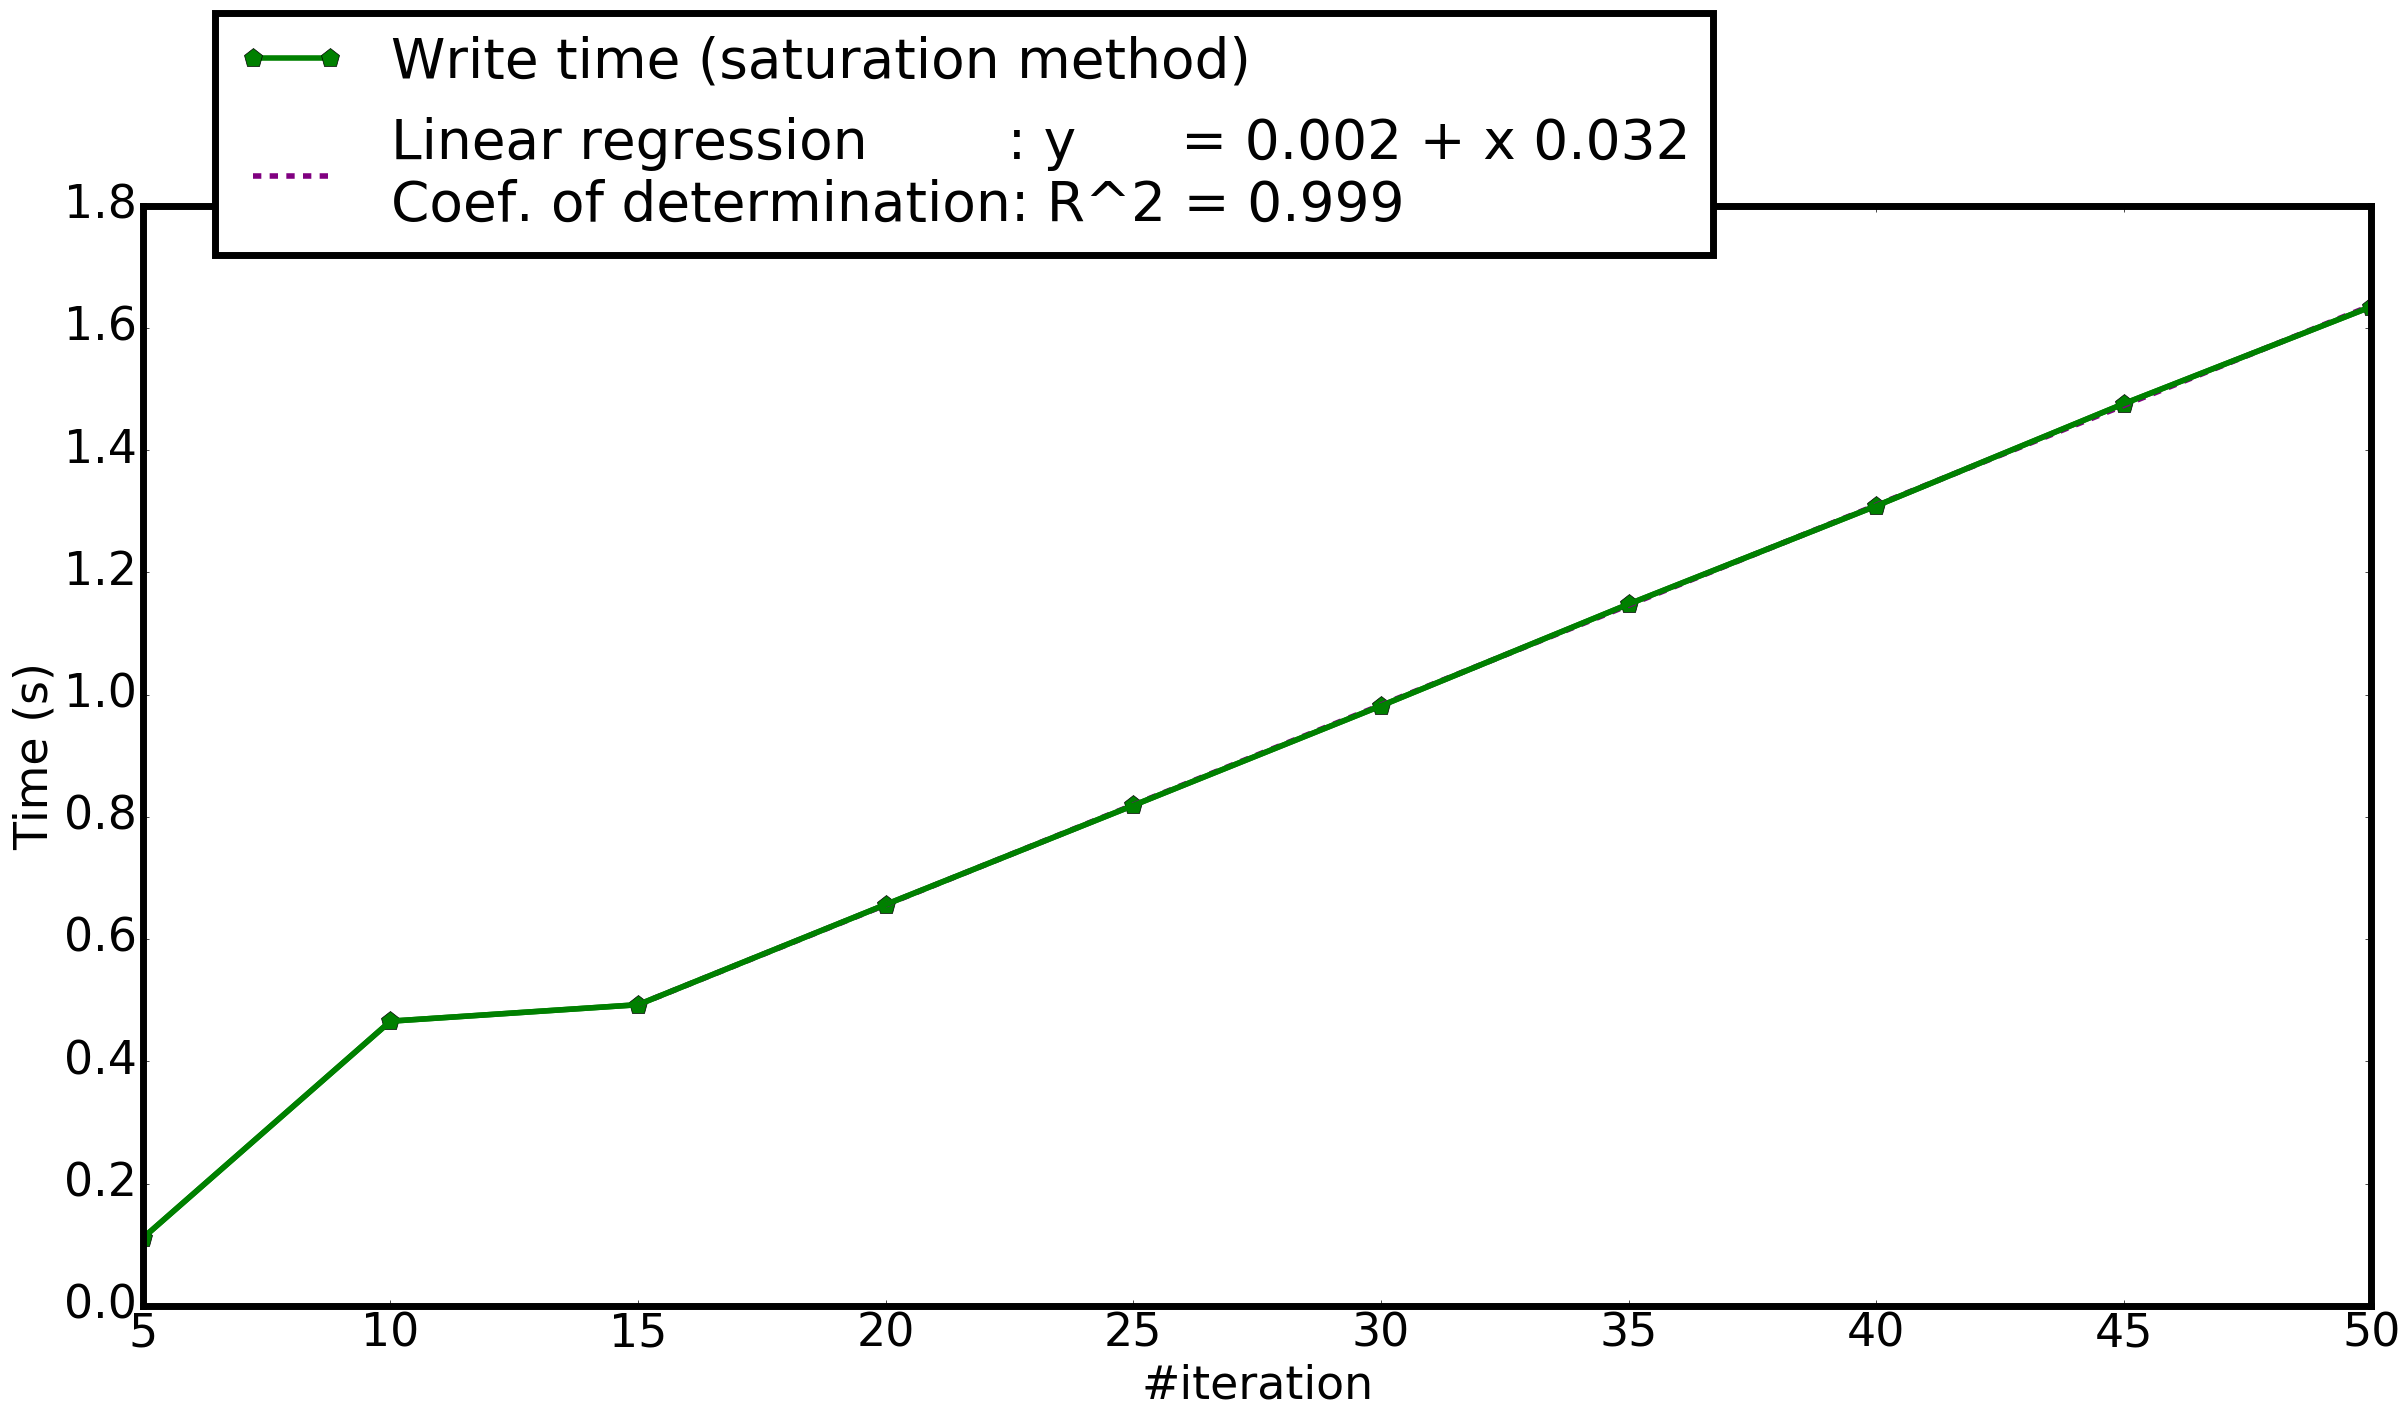
\includegraphics[width=\textwidth]{charts/writeTimeExample_saturationMethod_workstation_8core.png}
					\caption[\targetPlatformLaptop\space @ \targetPlatformLaptopFrequency]
					{{\small \targetPlatformLaptop\space @ \targetPlatformLaptopFrequency}}
				\end{subfigure}
				\hfill
				\begin{subfigure}[b]{0.475\textwidth}  
					\centering 
					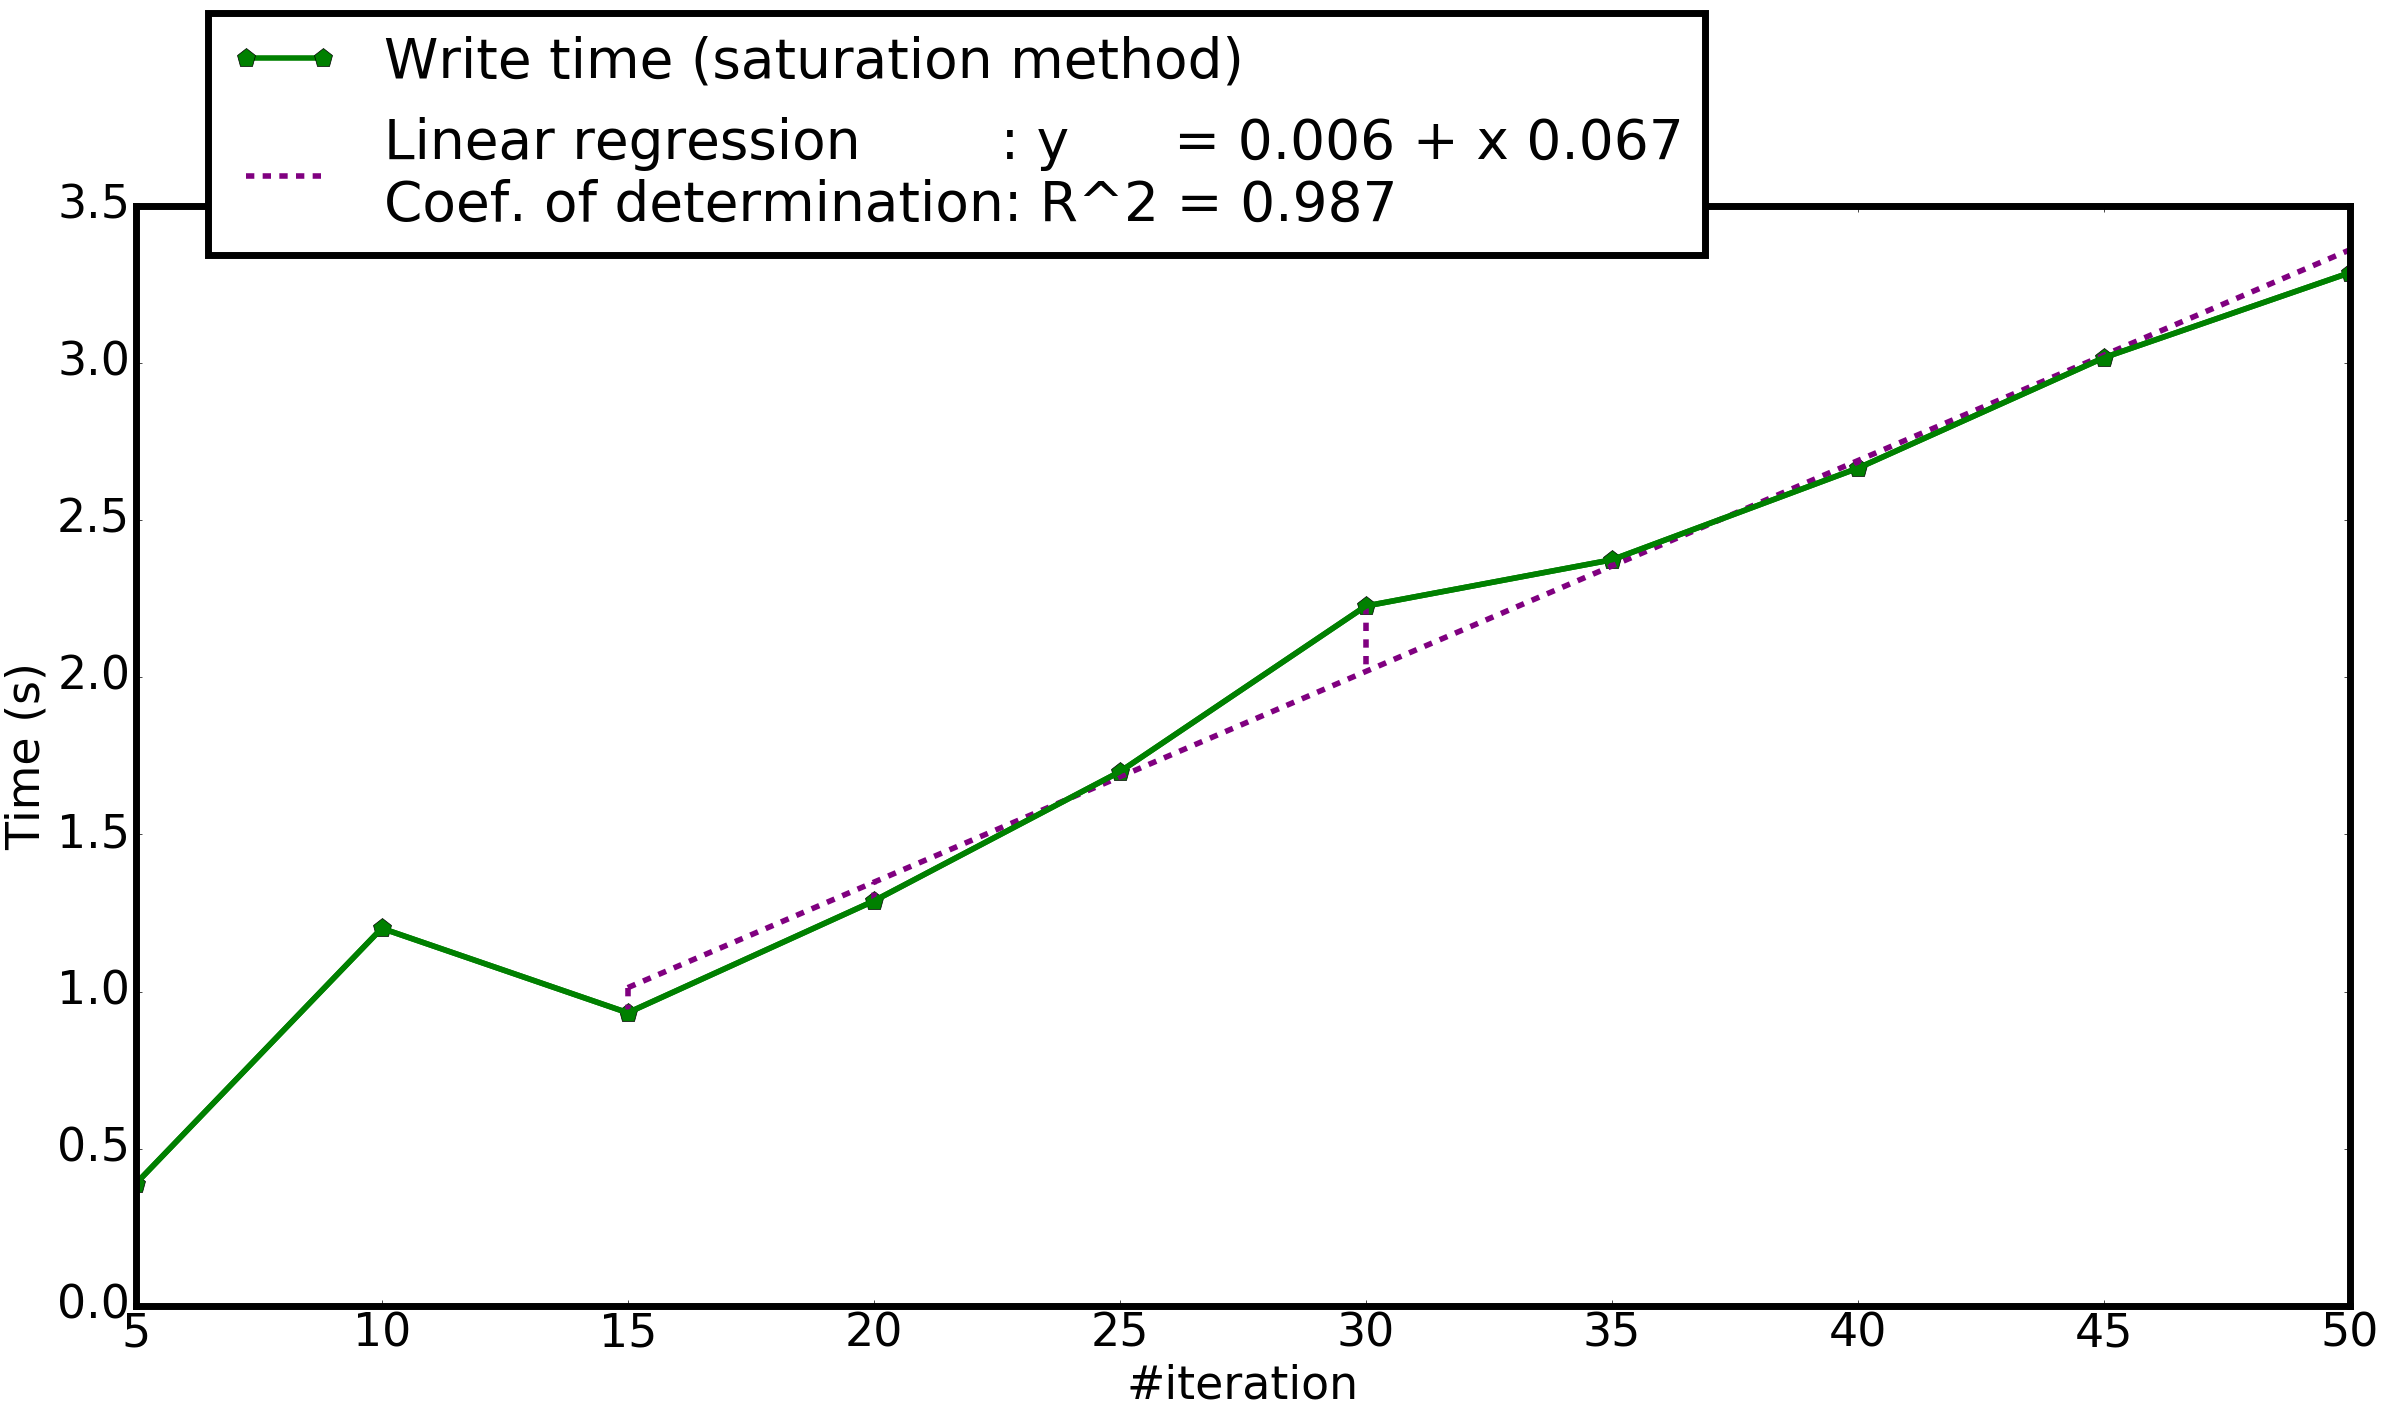
\includegraphics[width=\textwidth]{charts/writeTimeExample_saturationMethod_HPC_jureca.png}
					\caption[]%
					{{\small \targetPlatformHpc\space @ \targetPlatformHpcFrequency}}    
					\label{fig:writeTimeExample_saturation_hpc}
				\end{subfigure}
				\caption{Experimental assessment of the time for writing 50,000,000 bytes using the \emph{I/O saturation method}}
				\label{fig:writeTimeExample_saturation}
			\end{figure*}
			In Figure \ref{fig:writeTimeExample_saturation}, we have represented our measurement of the \emph{write} time ($50,000,000$ bytes) using the \emph{saturation method}.   One can notice that, after a warm-up phase\footnote{Corresponding to the time to flood the file system with \notationIO\space requests}, the \emph{write} time reaches a given threshold.   Then, its fluctuations almost vanish.\\

			Thanks to the \emph{saturation method}, the fitting-coefficient of the \emph{write} time estimation has been improved to $0.987$ (see Figure \ref{fig:writeTimeExample_saturation_hpc}) on the \targetPlatformHpc\space platform.   Furthermore, the constant term in the linear approximation of the \emph{write} time is now closer to zero ($0.006$ seconds) compared to the previous value of $1.42$ seconds (see Figure \ref{fig:writeTimeExample_hpc}).   Therefore, the following linear function:
				\begin{equation*}
				\begin{aligned}
					f(iteration) = W_{perturbation} * iteration
				\end{aligned}
				\end{equation*}
			is more realistic.\\
			Note that the currently-presented experimentation has been obtained by excluding, in the linear regression, the samples which are bellow the worm-up threshold (two first points).   This is done in order to remove any bias which would be introduced during the warm-up phase to our linear regression.\\

			Thanks to this \emph{saturation method}, we have a more stable and more realistic evaluation of the \emph{write} time.   However, it is clear that this measured value is artificially increased; hence the importance to show its constancy\footnote{Fitness of the linear regression with the experimental points}.   Indeed, a constant overhead in the \emph{write} time (for all the experimentations) will not affect a benchmark study as long as it is incorporated in \emph{all} the compared algorithms.


		\subsubsection{Modelling the \notationaio\space request time ($req$)}
			Here, we evaluate the time needed to submit an \notationaio\space request on the considered hardware platform.   Let us also check the validity of its constancy (stated in Section \ref{subsubsection:modelRequestTime}) with respect to the number of submitted requests).\\

				\begin{figure*}[!h]
					\centering
					\begin{subfigure}[b]{0.475\textwidth}
						\centering
						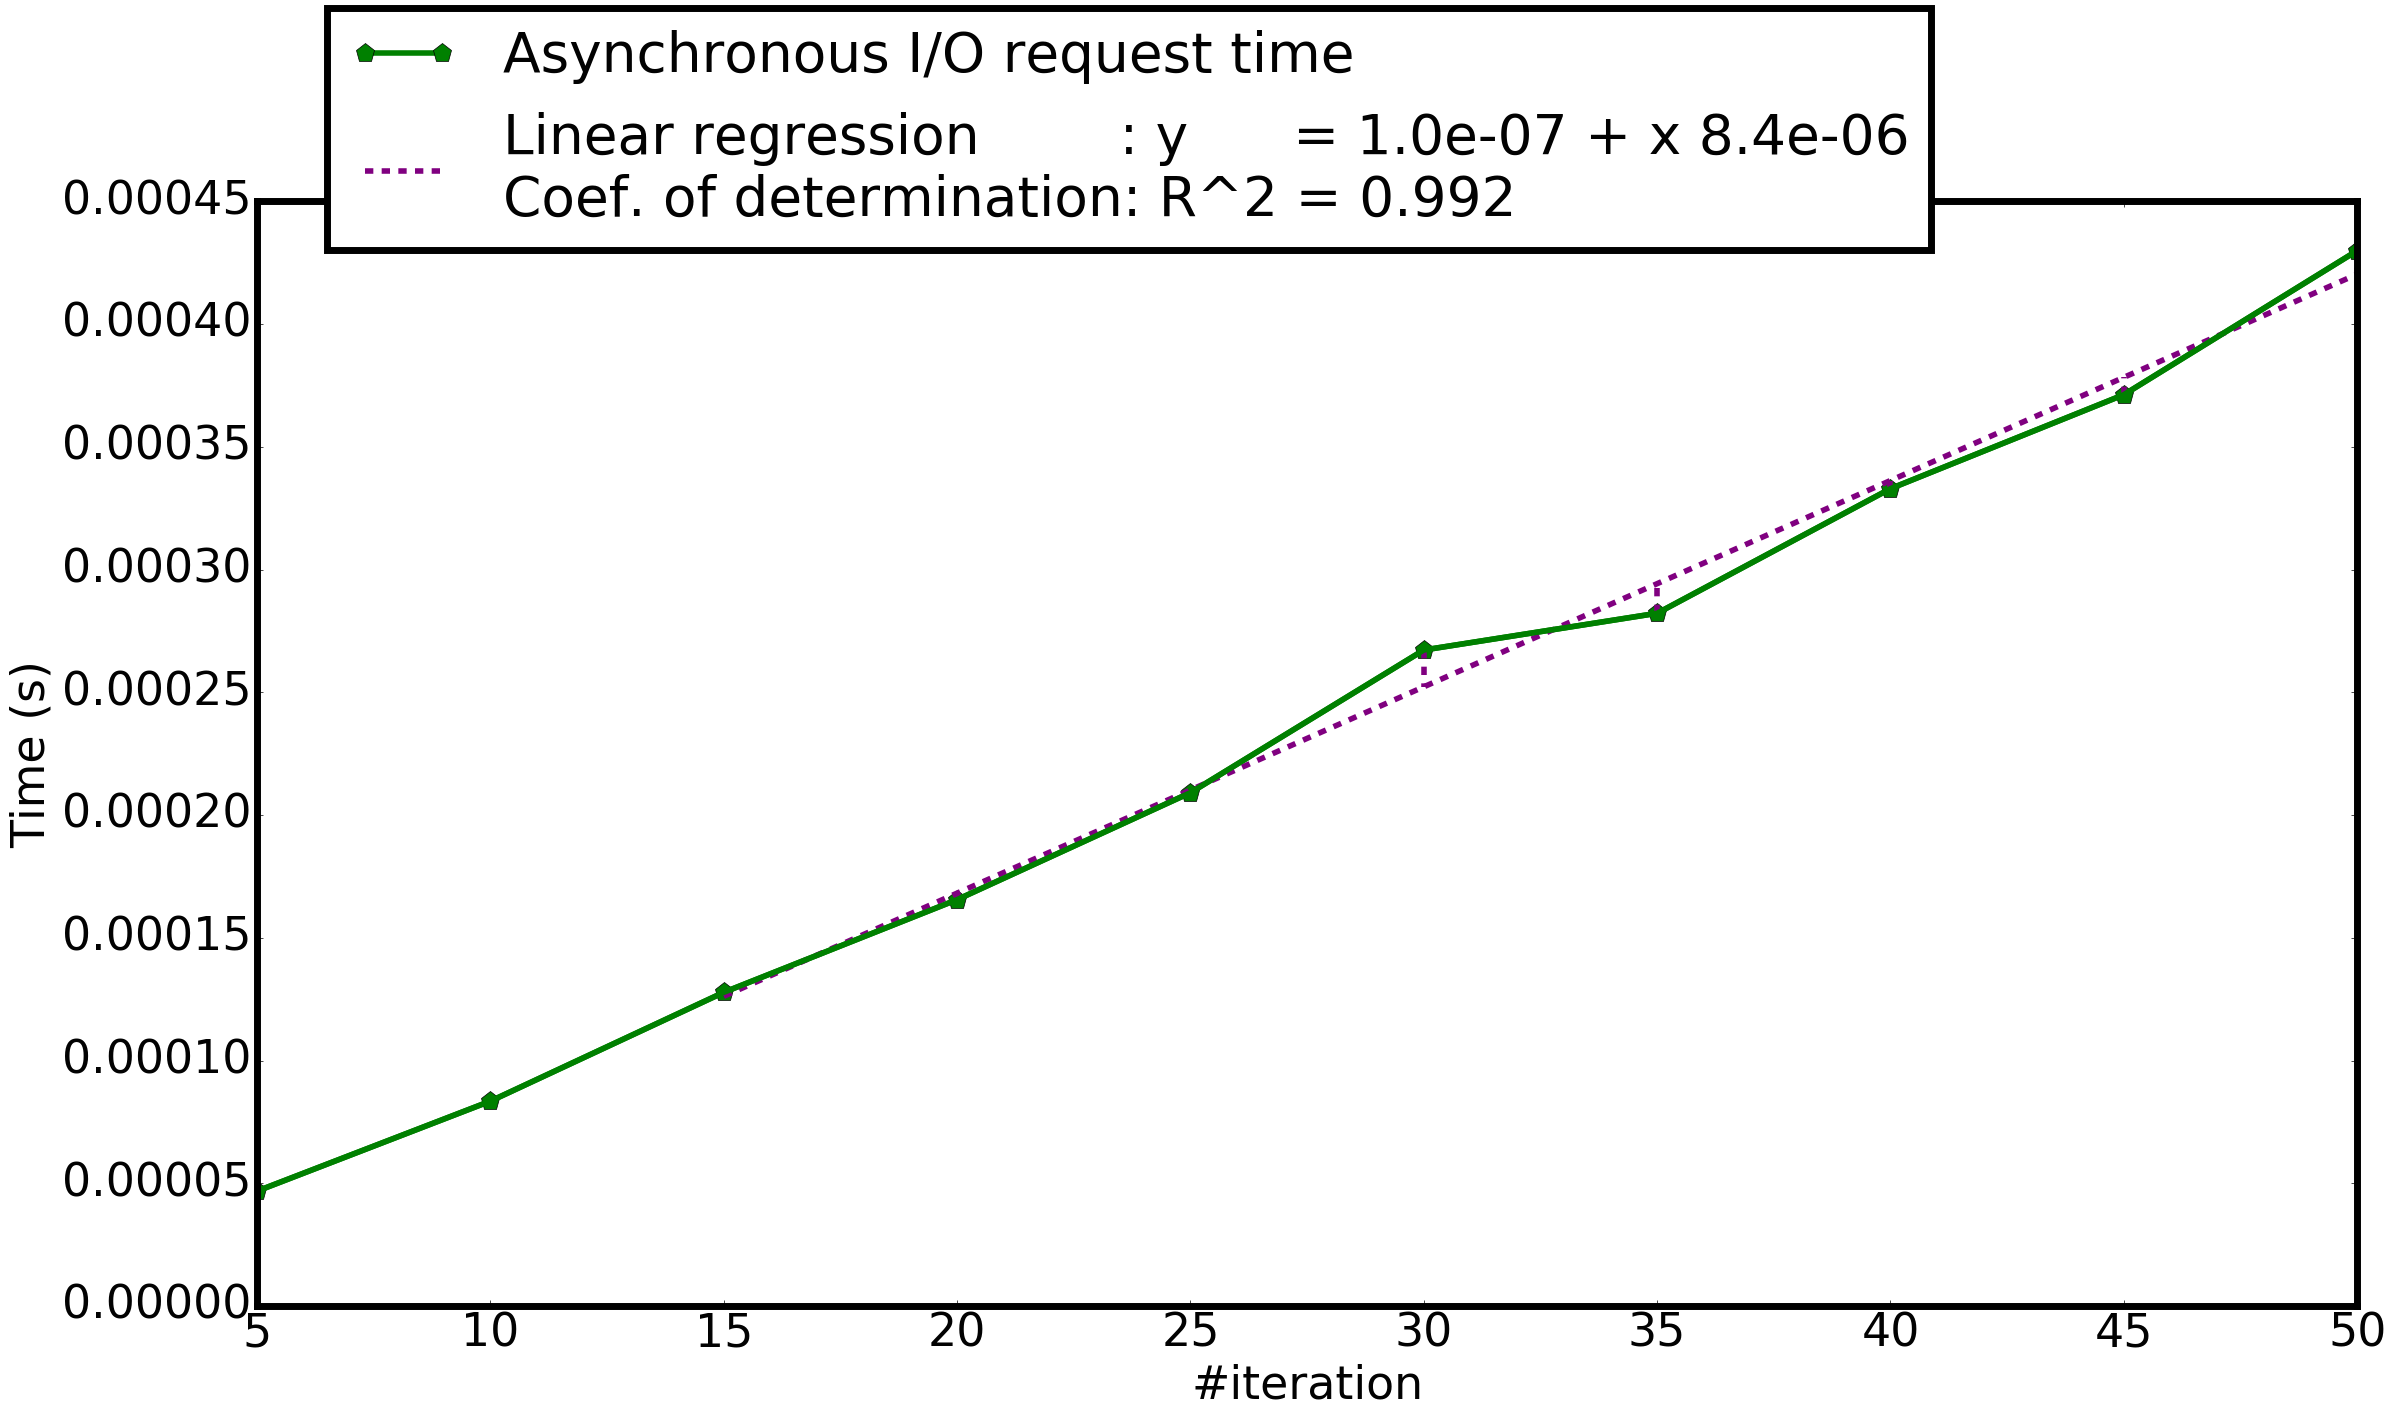
\includegraphics[width=\textwidth]{charts/requestTimeExample_workstation_8core.png}
						\caption[\targetPlatformLaptop\space @ \targetPlatformLaptopFrequency]
						{{\small \targetPlatformLaptop\space @ \targetPlatformLaptopFrequency}}
					\end{subfigure}
					\hfill
					\begin{subfigure}[b]{0.475\textwidth}  
						\centering 
						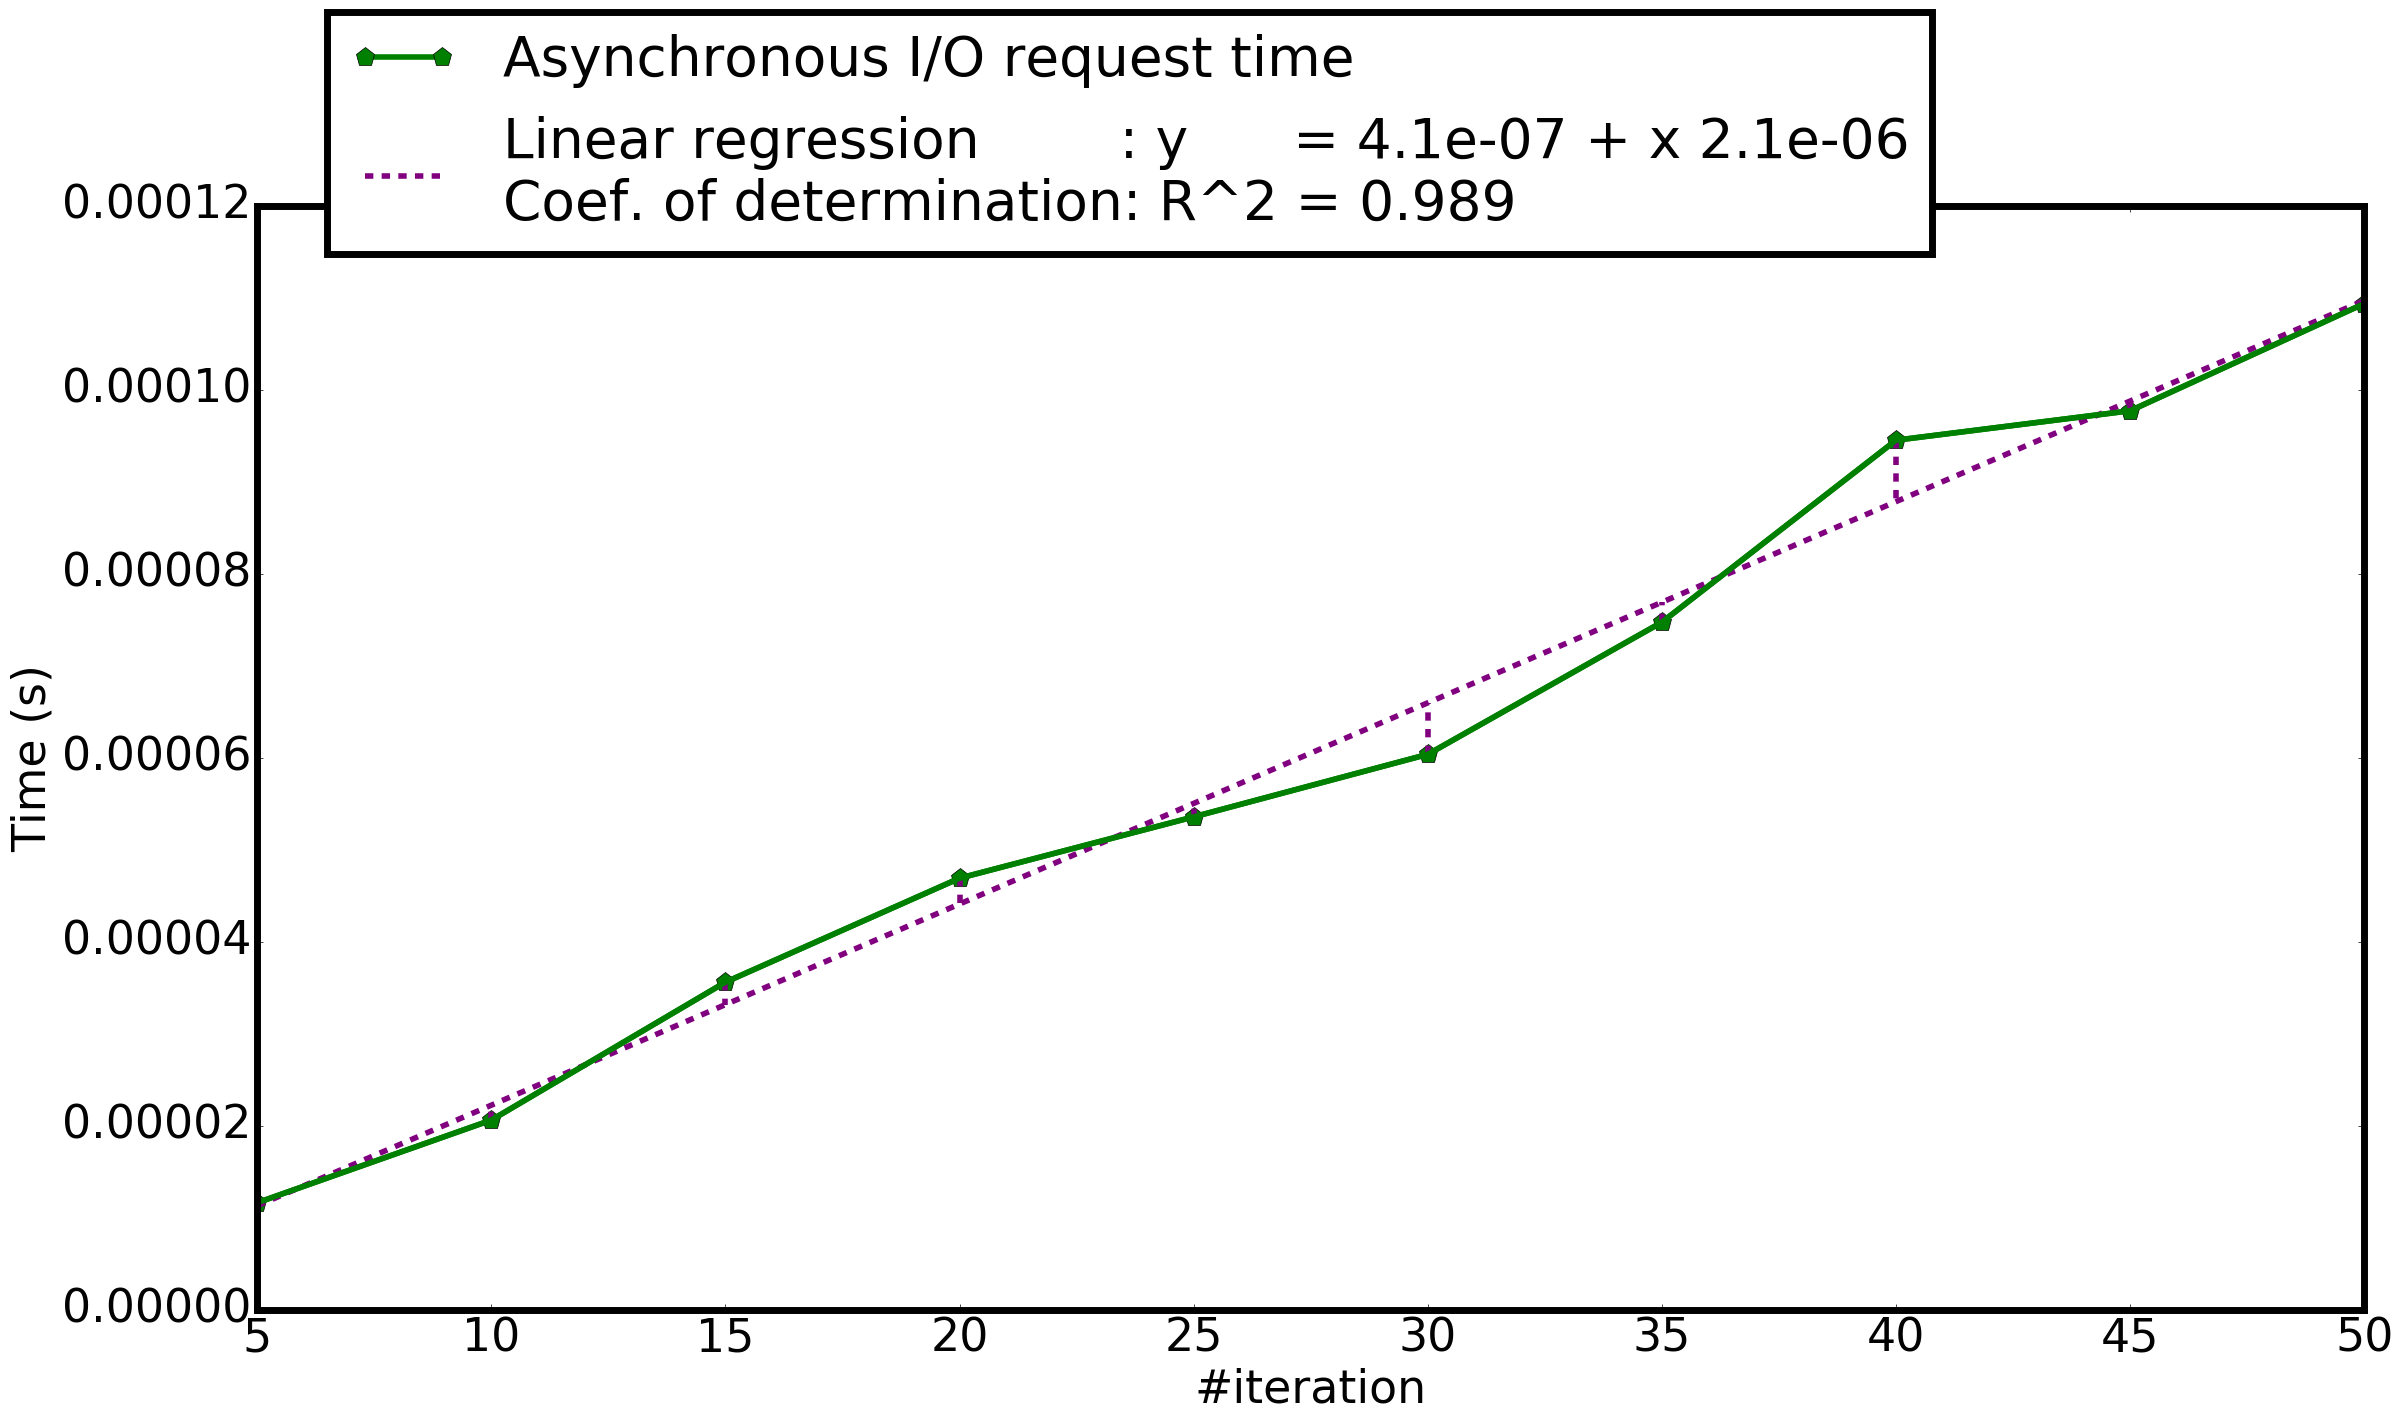
\includegraphics[width=\textwidth]{charts/requestTimeExample_hpc.png}
						\caption[]%
						{{\small \targetPlatformHpc\space @ \targetPlatformHpcFrequency}}    
					\end{subfigure}
					\caption{Experimental assessment of the time for forwarding a request to the asynchronous \notationaioWriteThread}
					\label{fig:requestTimeExample}
				\end{figure*}

			In Figure \ref{fig:requestTimeExample}, we present our experimental evaluation of the \notationaio\space request time ($req$) within the two considered hardware platforms.   Using the numerical method described in Section \ref{subsubsection:modelRequestTime}, we estimate the value of the request time as well as the validity of the hypothesis: constant request time (for a given hardware platform).

			The value of $req$ is the slop of the linear regression (Figure \ref{fig:requestTimeExample}).   This value is, respectively, $8.4 e^{-6}$ seconds and $2.1 e^{-6}$ seconds for the \targetPlatformLaptop\space and the \targetPlatformHpc\space platform.   Moreover, the \emph{coefficient of determination} ($R^{2}=0.992$ and $R^{2}=0.989$) do not contradict our hypothesis about the constancy of the \notationaio\space request time.



%--------------------------------------------
\section{Real-life experimental case: the \toolTargetSoftware}\label{section:experimentalCase}
	Let us now see how the previously presented results may be transposed to a real-life example: the \toolTargetSoftware.\\
	The objective of this section is to check whether the previously noticed improvements brought by our asynchronous \emph{write} implementation may still be achieved within a real-life application.   We also aim to identify any additional perturbation that our \notationaio\space solution may introduce on a general-purpose computation.    In a second step, we evaluate our custom solutions to eliminate (or at least to reduce) these undesirable interferences.\\

	All the presented experimental results are obtained following the same protocol.   Each considered point is assessed (experimental run) 10 times in a row.   The presented corresponding value is the average of the result of these 10 runs.   We also present an error bar showing the distance between the maximal and minimal value of these 10 runs.\\
	It is also worthwhile to mention that for all the following experimentations, the used inputs\footnote{Performance profile file (see Section \ref{section:workingFramework})} of the \toolTargetSoftware\space have not been processed nor modified.   Thus, the observed executions of the \toolTargetSoftware\space are performed in a real-life conditions and with real-life data samples.\\
	All the used input data samples (performance profiling file) have been obtained by profiling the execution of the \emph{NAS parallel benchmark}\footnote{Set of programs designed by \emph{NASA} to help evaluate the performance of parallel supercomputers. The benchmarks are derived from computational fluid dynamics (CFD) applications}.   They all represent the execution of about $10^{5}$ threads.   Each file is about $10^{9}$ Bytes large.


	\subsection{Basic POSIX-based asynchronous implementation}
		In this first step, we embed our basic asynchronous writing strategy within the \toolTargetSoftware.   The experimental assessments of this implementation are compared in Figures \ref{fig:cubeRemapper_basicImplementation_write} and \ref{fig:cubeRemapper_basicImplementation_compute_total} to the state-of-the-art (synchronous) implementation of the \toolTargetSoftware\space.\\

			\begin{figure*}[!h]
				\centering
				\begin{subfigure}[b]{0.475\textwidth}
					\centering
					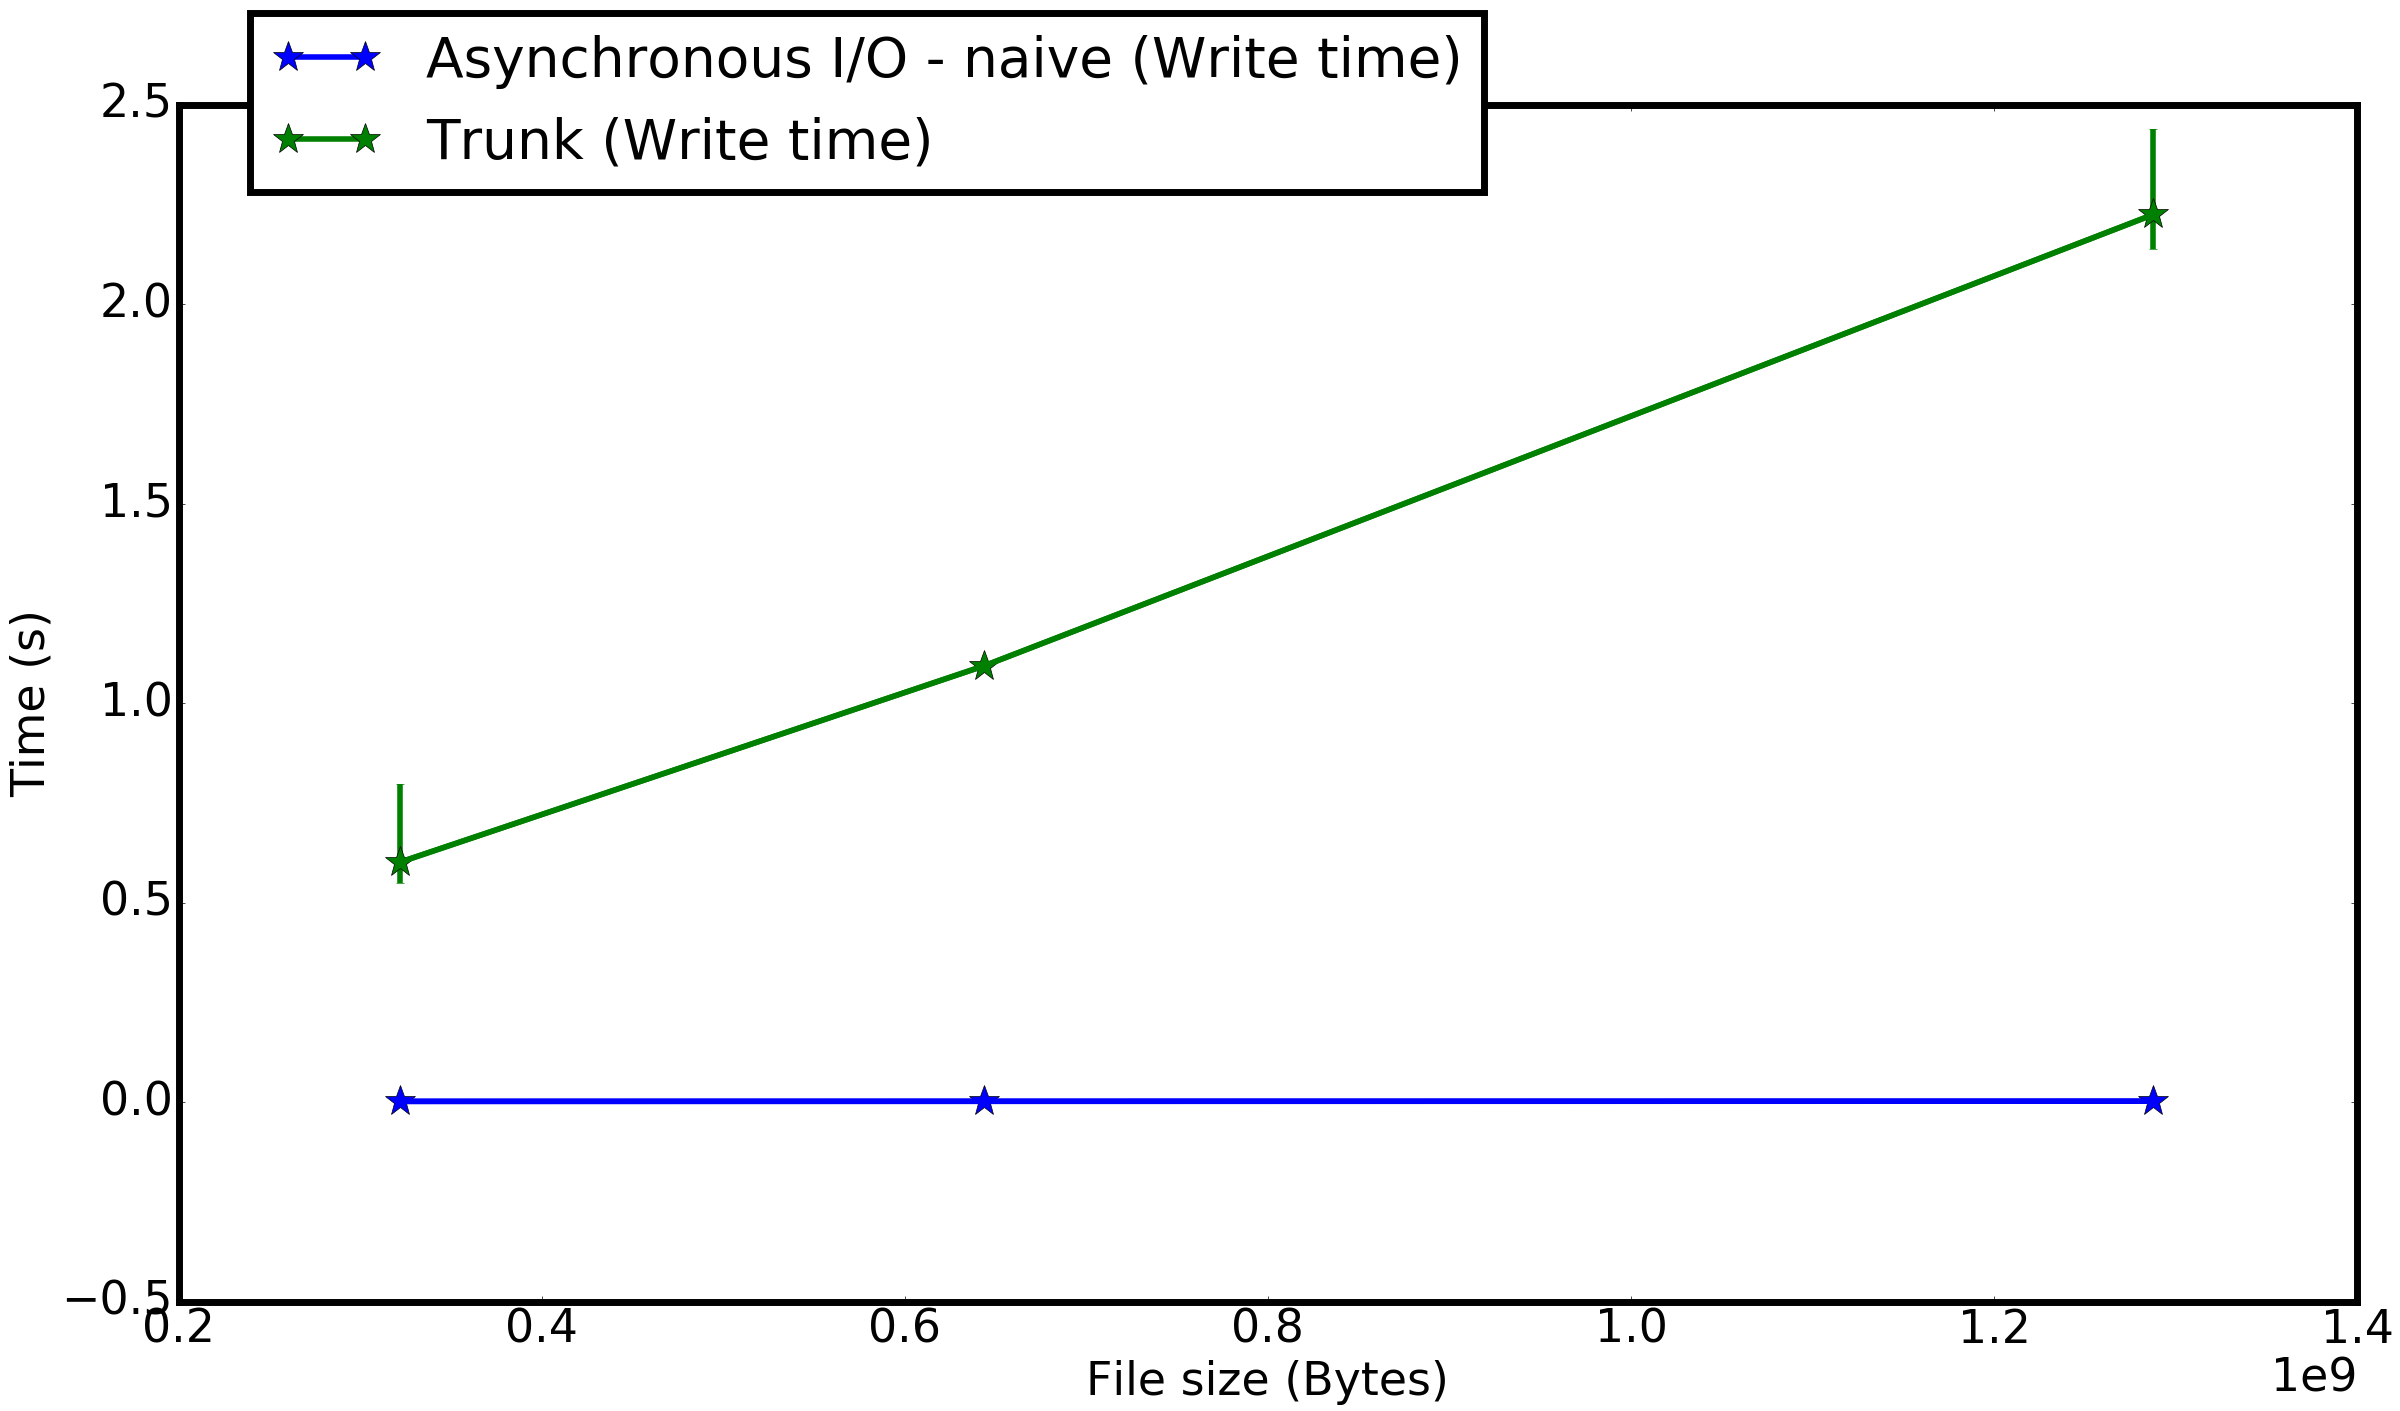
\includegraphics[width=\textwidth]{charts/cubeRemapper_basicImplementation_write_workstation_8core.png}
					\caption[\targetPlatformLaptop \space @ \targetPlatformLaptopFrequency]
					{{\small \targetPlatformLaptop \space @ \targetPlatformLaptopFrequency}}
				\end{subfigure}
				\hfill
				\begin{subfigure}[b]{0.475\textwidth}
					\centering
					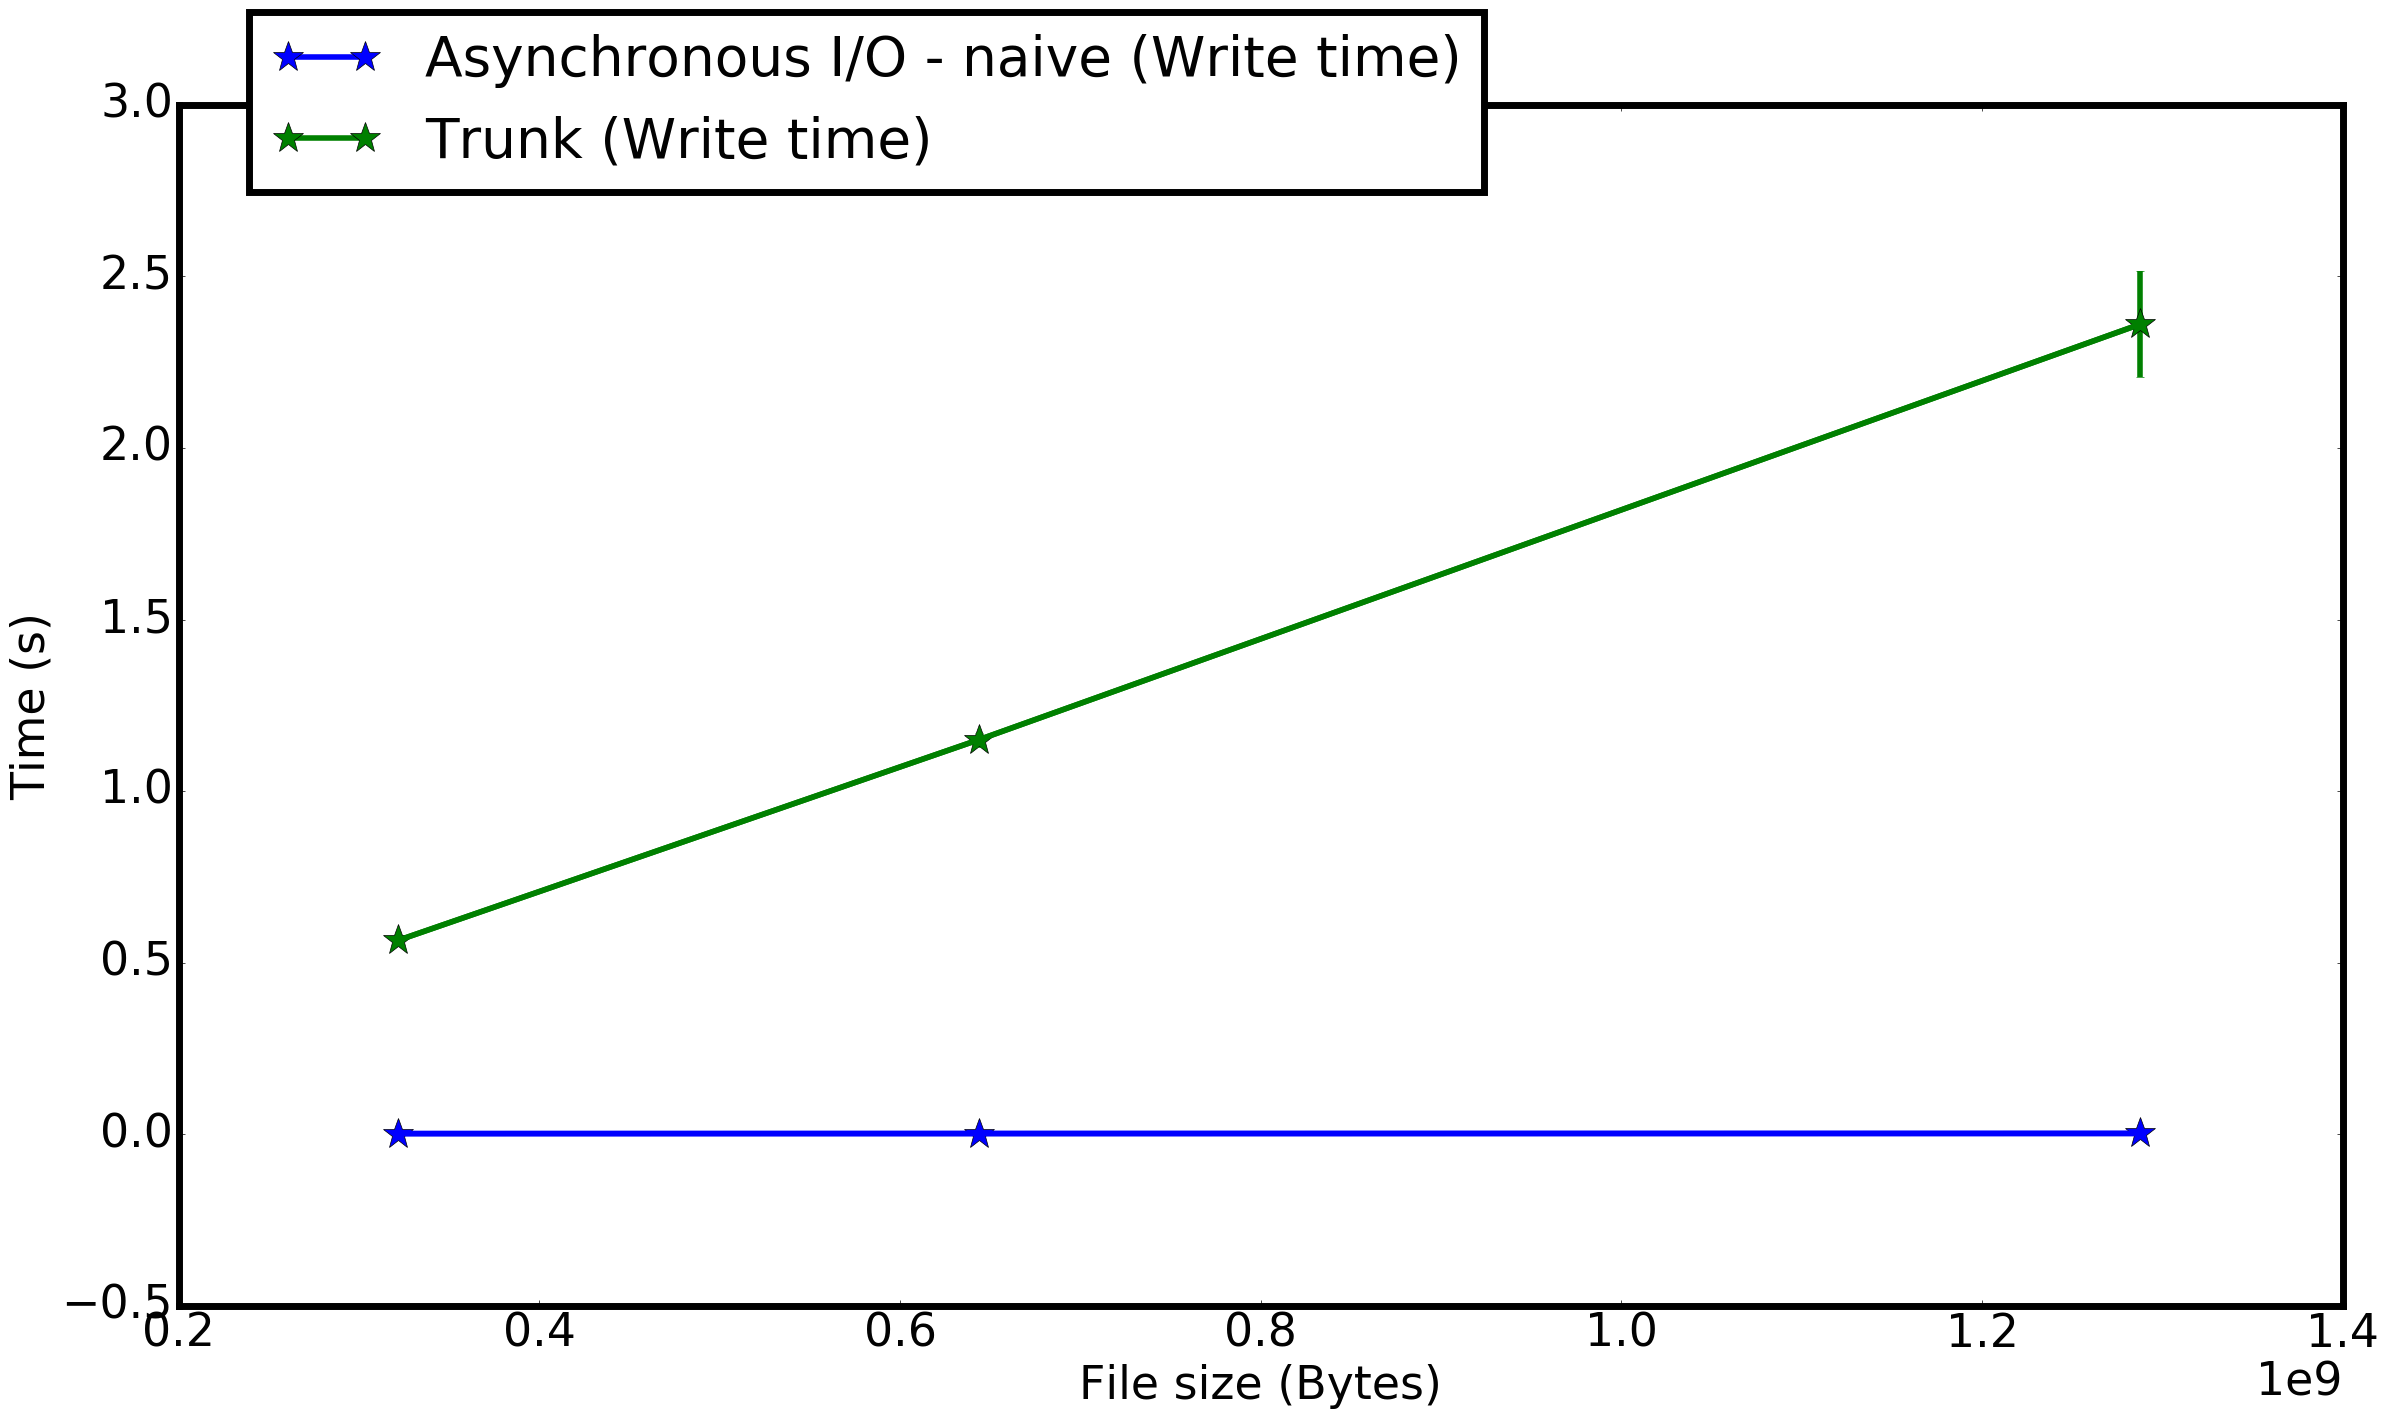
\includegraphics[width=\textwidth]{charts/cubeRemapper_basicImplementation_write_hpc.png}
					\caption[]%
					{{\small \targetPlatformHpc \space @ \targetPlatformHpcFrequency}}
				\end{subfigure}
				\caption{Experimental comparison of the \emph{write} time: proposed \emph{\notationaio\space} (naive) VS. \emph{state-of-the-art} (trunk synchronous) implementation of the \toolTargetSoftware}
				\label{fig:cubeRemapper_basicImplementation_write}
			\end{figure*}

		As one could expect, Figure \ref{fig:cubeRemapper_basicImplementation_write} shows that the \emph{write} time of our custom basic implementation is now almost null (compared to the synchronous \emph{write} time).   Instead of waiting for a costly \notationIO\space \emph{write} time at each iteration, we simply wait for the time to enqueue a request within a shared queue.   Given the reduced \emph{write} time (compared to the \emph{compute} time), the \notationaio\space strategy has a negligible final waiting\footnote{Time to wait for the pending \notationaio\space request to be executed once all the \emph{compute} operations have been executed} time.\\

			\begin{figure*}[!h]
				\centering
				\begin{subfigure}[b]{0.475\textwidth}
					\centering
					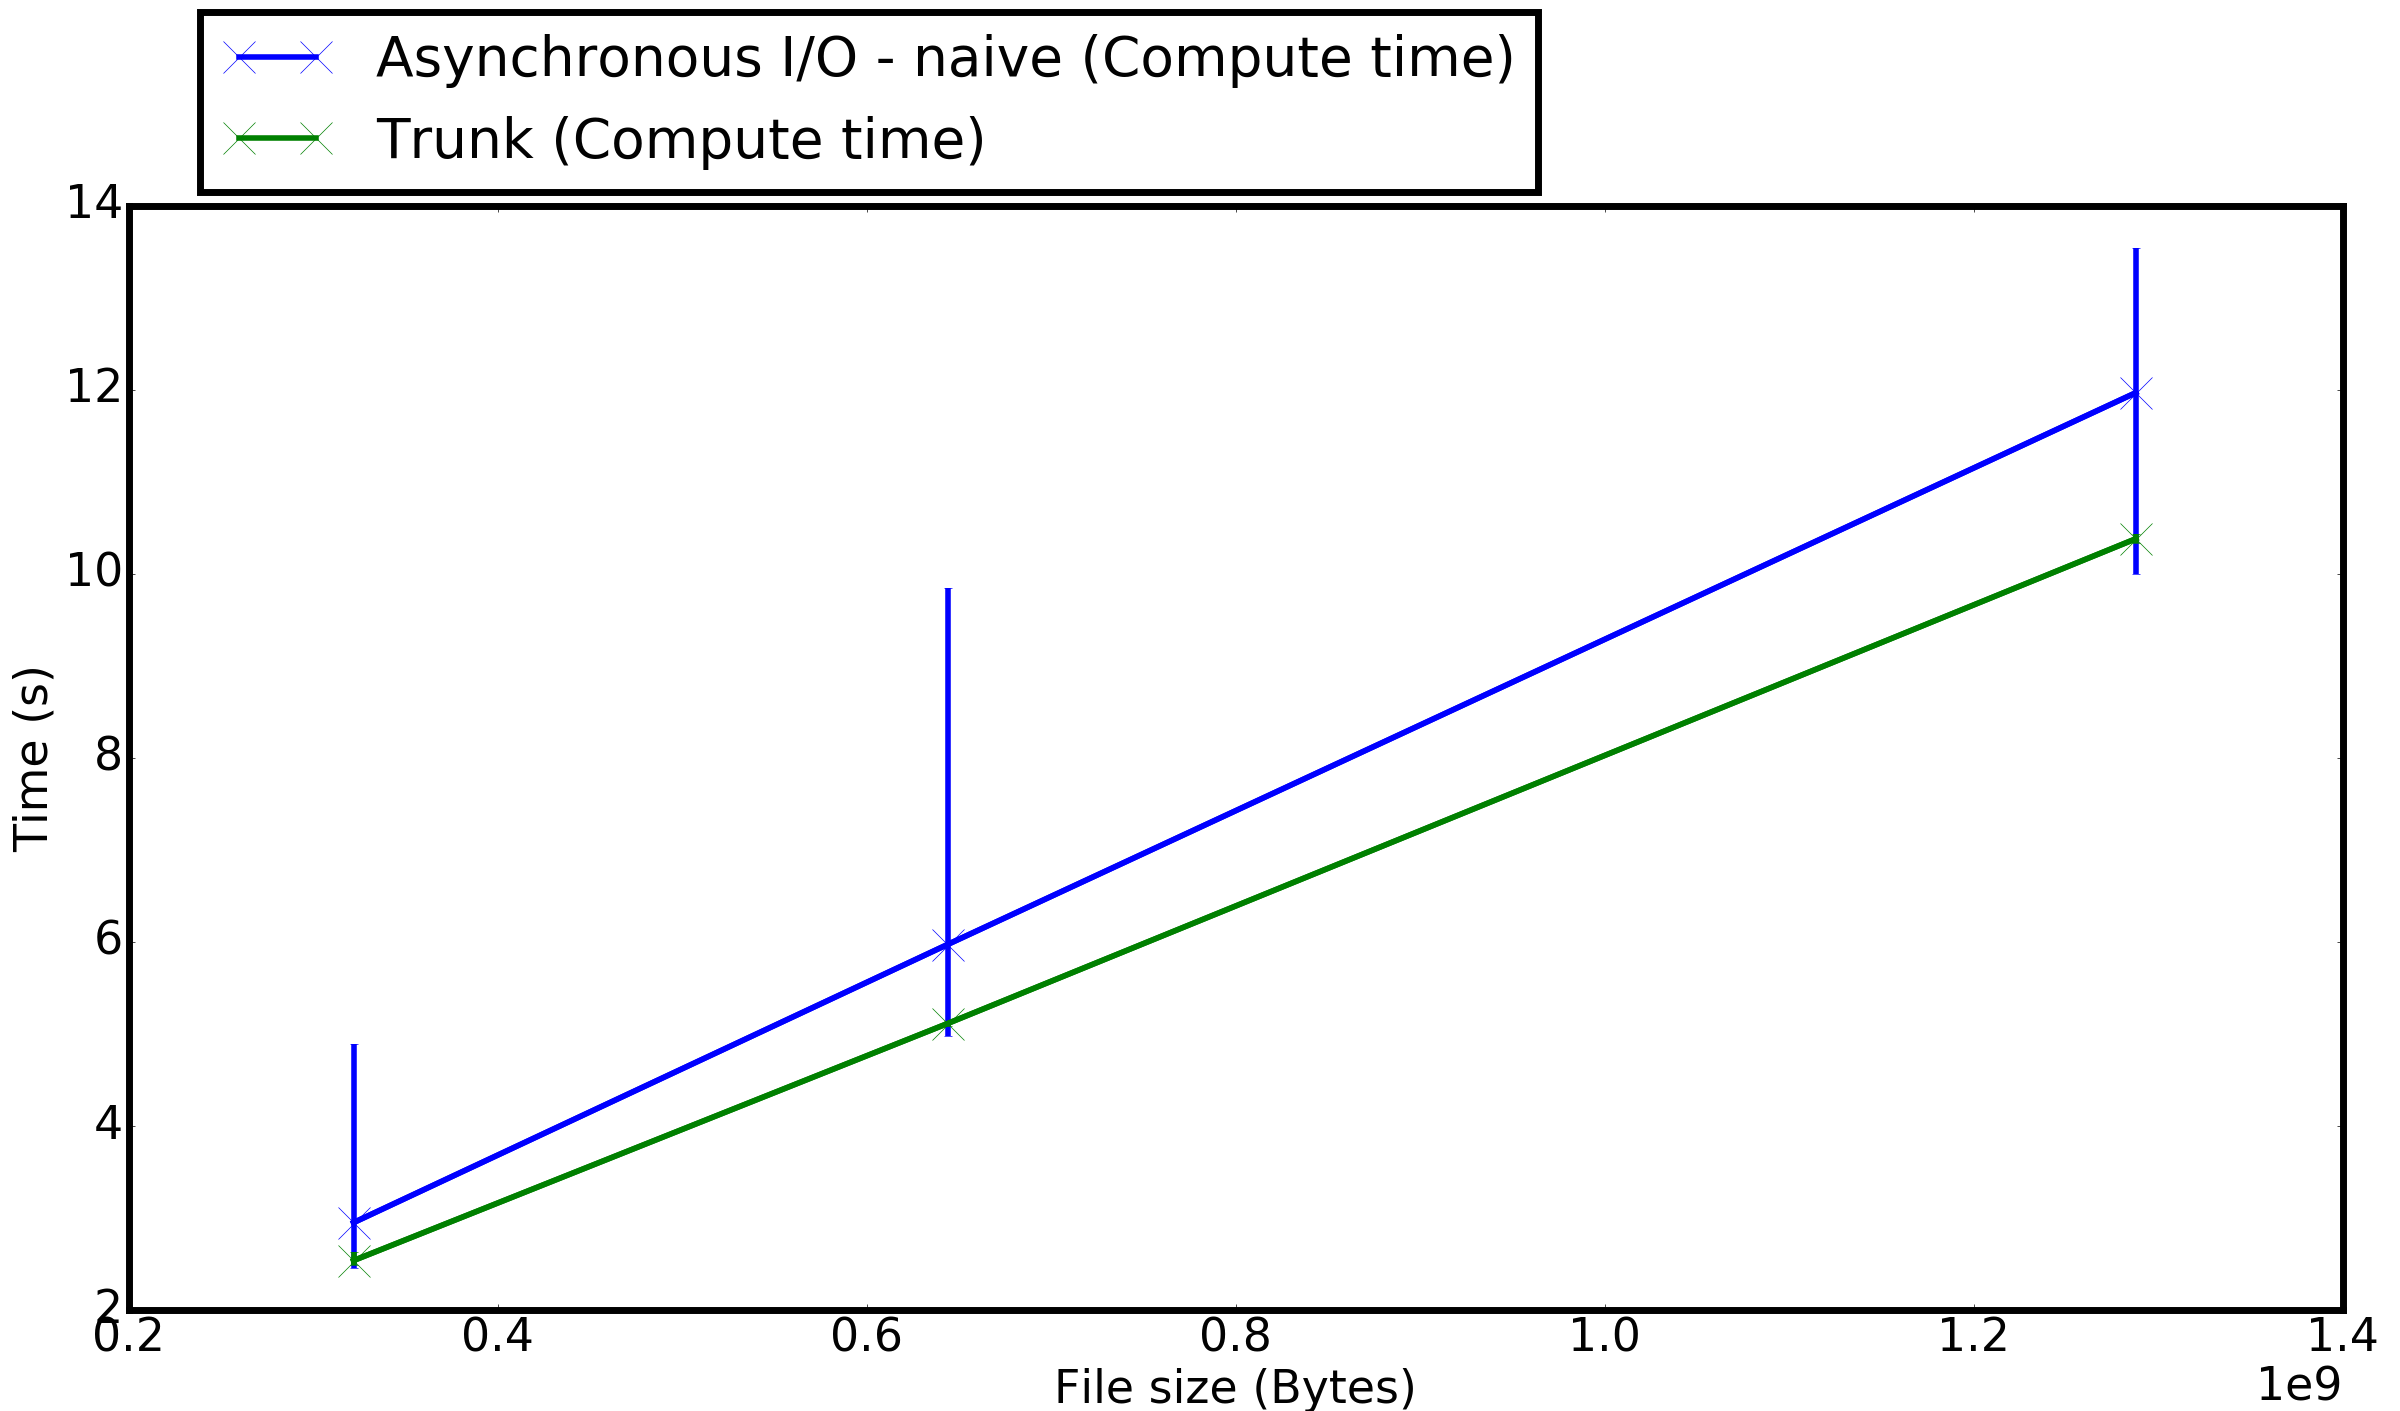
\includegraphics[width=\textwidth]{charts/cubeRemapper_basicImplementation_compute_workstation_8core.png}
					\caption[\targetPlatformLaptop \space @ \targetPlatformLaptopFrequency]
					{{\small \targetPlatformLaptop \space @ \targetPlatformLaptopFrequency}}
					\label{fig:cubeRemapper_basicImplementation_compute_workstation_8core}
				\end{subfigure}
				\hfill
				\begin{subfigure}[b]{0.475\textwidth}
					\centering
					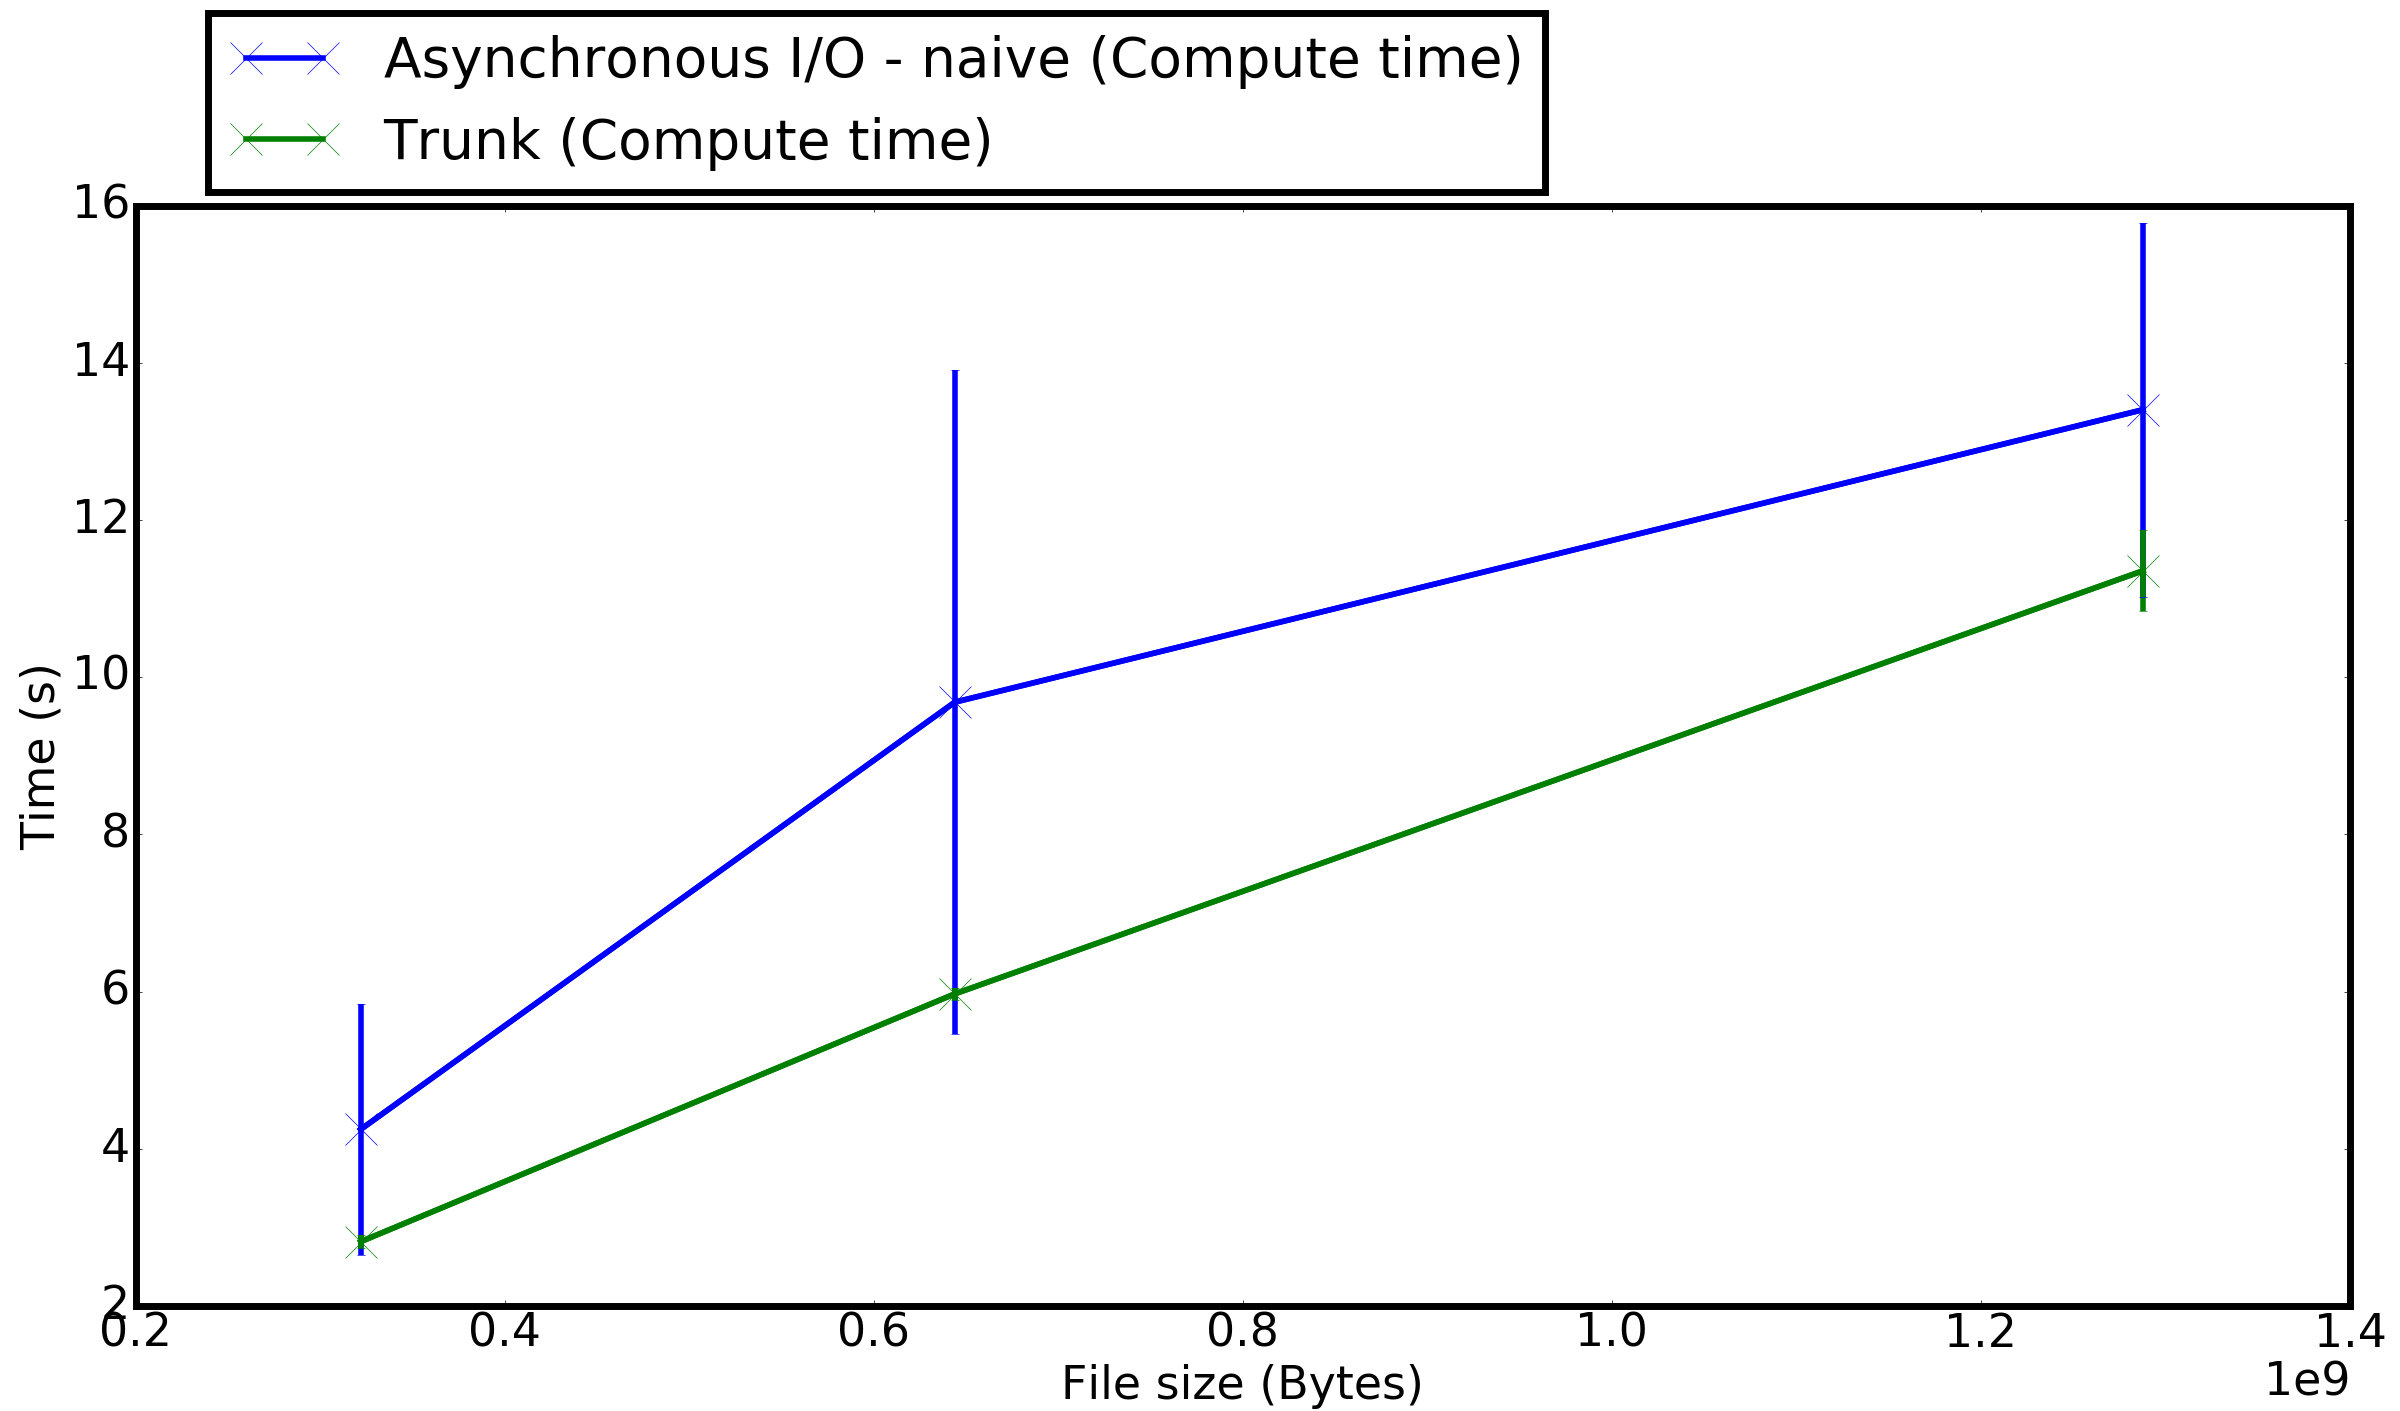
\includegraphics[width=\textwidth]{charts/cubeRemapper_basicImplementation_compute_hpc.png}
					\caption[]%
					{{\small \targetPlatformHpc \space @ \targetPlatformHpcFrequency}}    
					\label{fig:cubeRemapper_basicImplementation_compute_hpc}
				\end{subfigure}
				\hfill
				\begin{subfigure}[b]{0.475\textwidth}
					\centering
					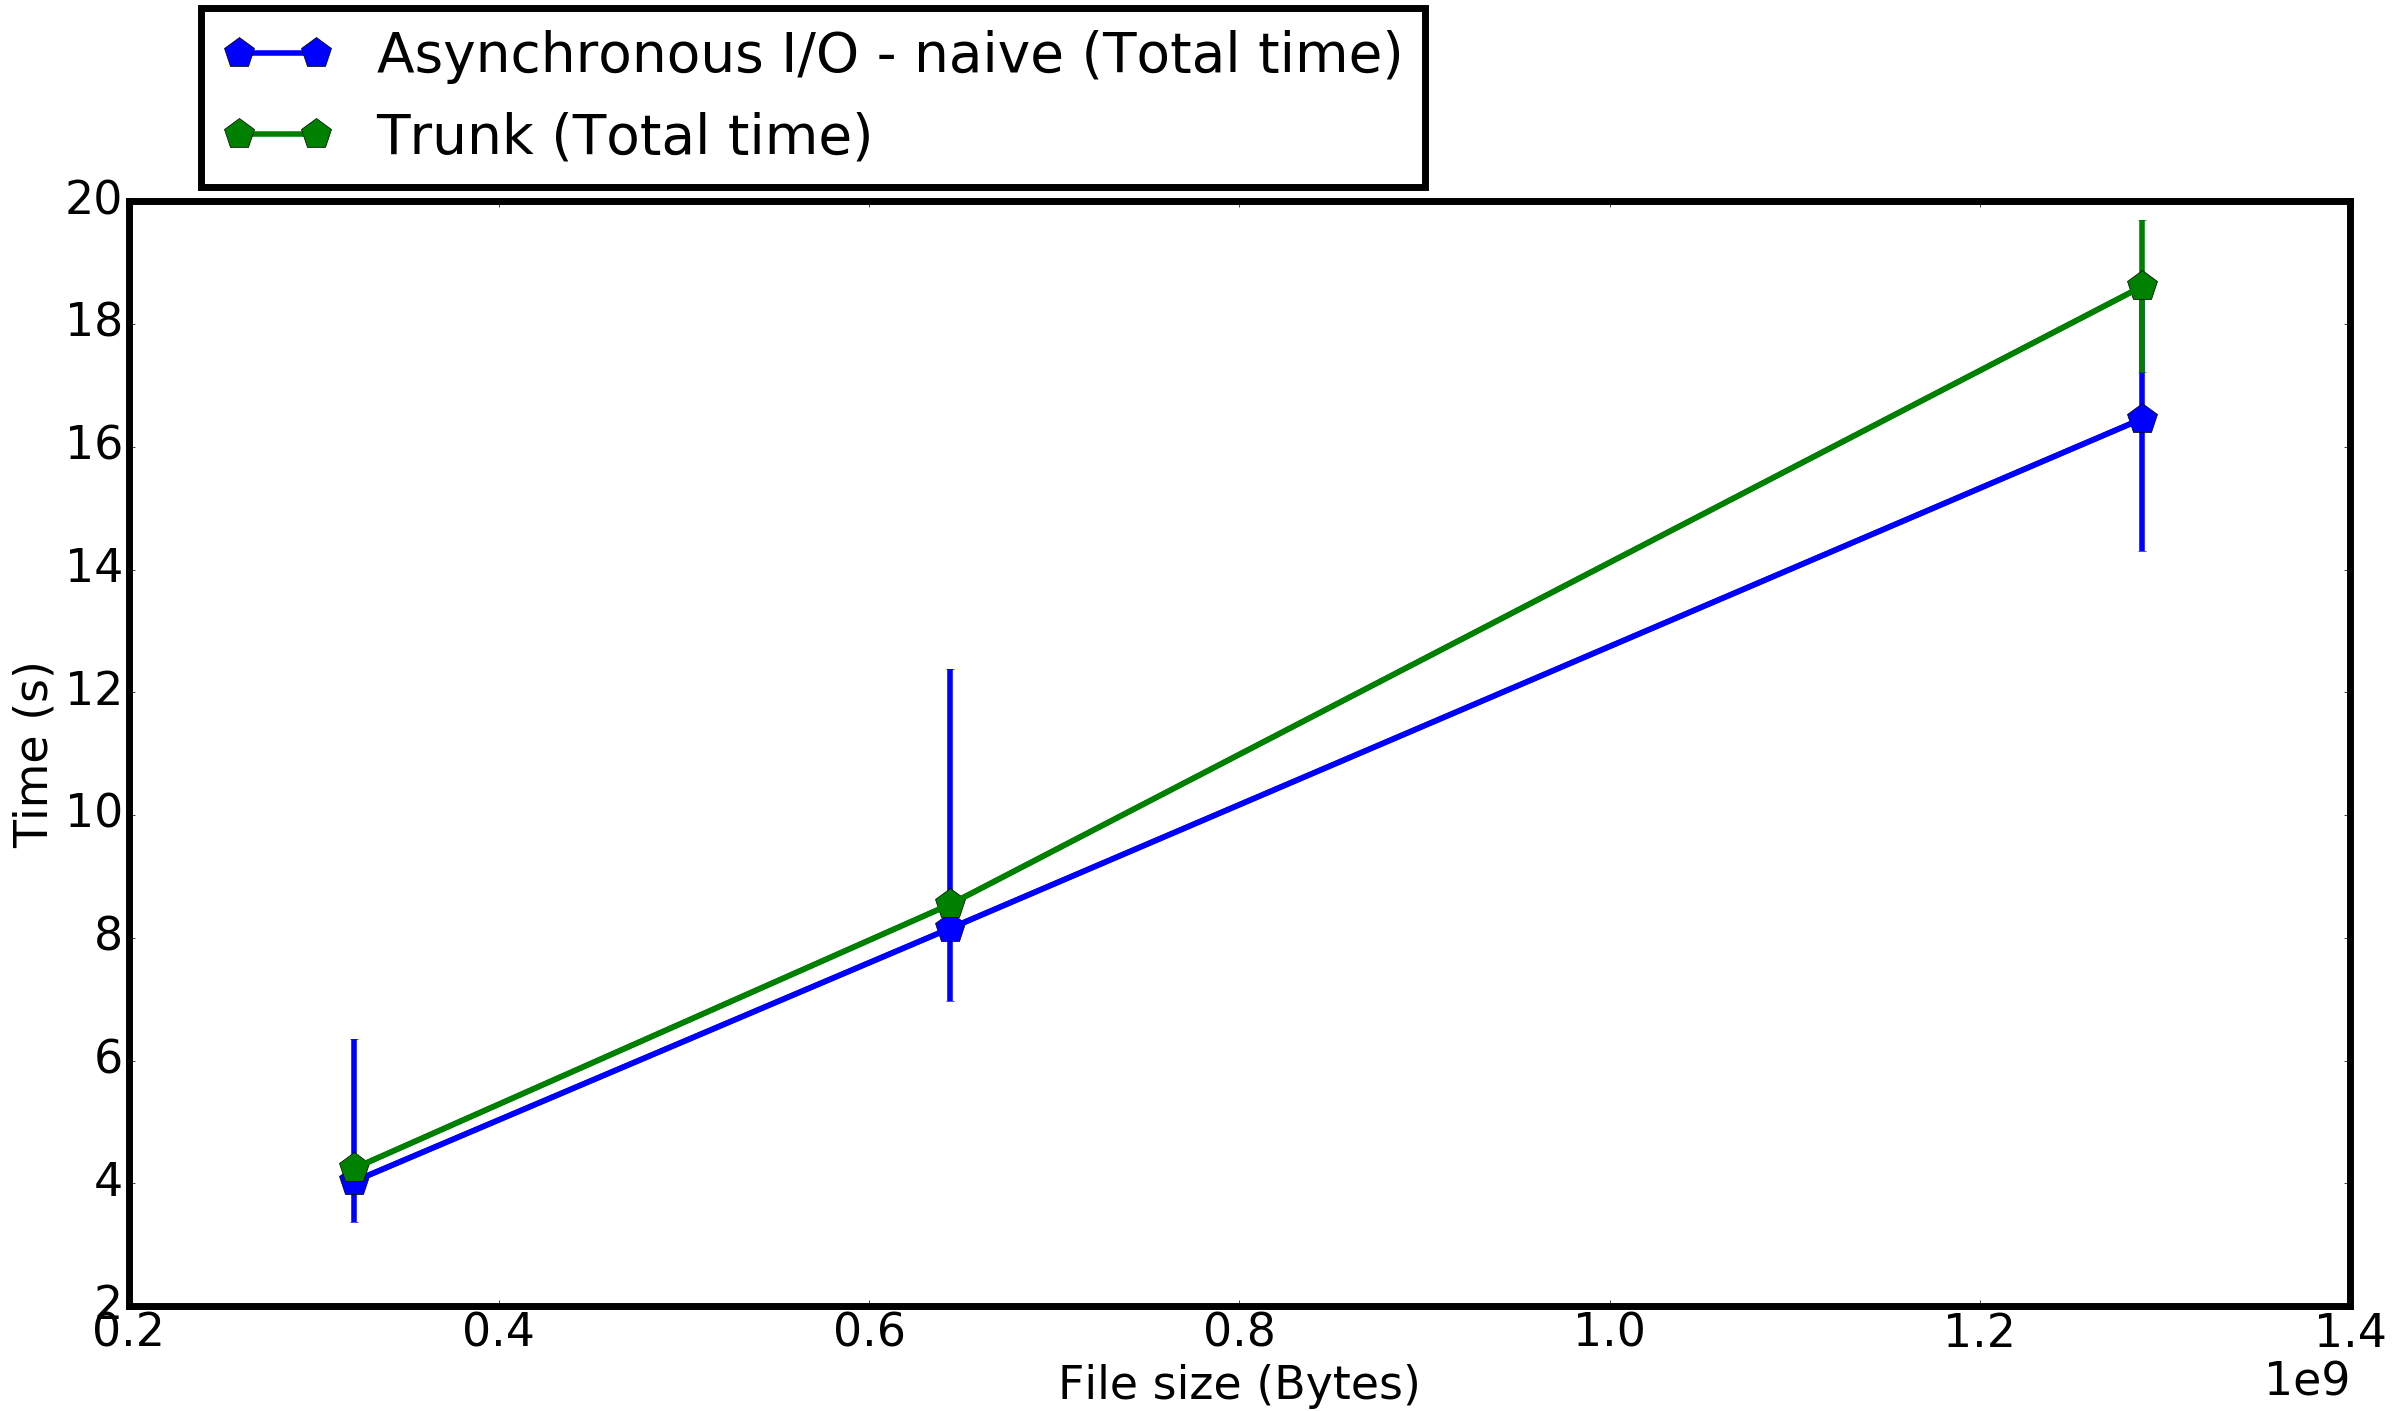
\includegraphics[width=\textwidth]{charts/cubeRemapper_basicImplementation_total_workstation_8core.png}
					\caption[\targetPlatformLaptop \space @ \targetPlatformLaptopFrequency]
					{{\small \targetPlatformLaptop \space @ \targetPlatformLaptopFrequency}}
					\label{fig:cubeRemapper_basicImplementation_total_workstation_8core}
				\end{subfigure}
				\hfill
				\begin{subfigure}[b]{0.475\textwidth}
					\centering
					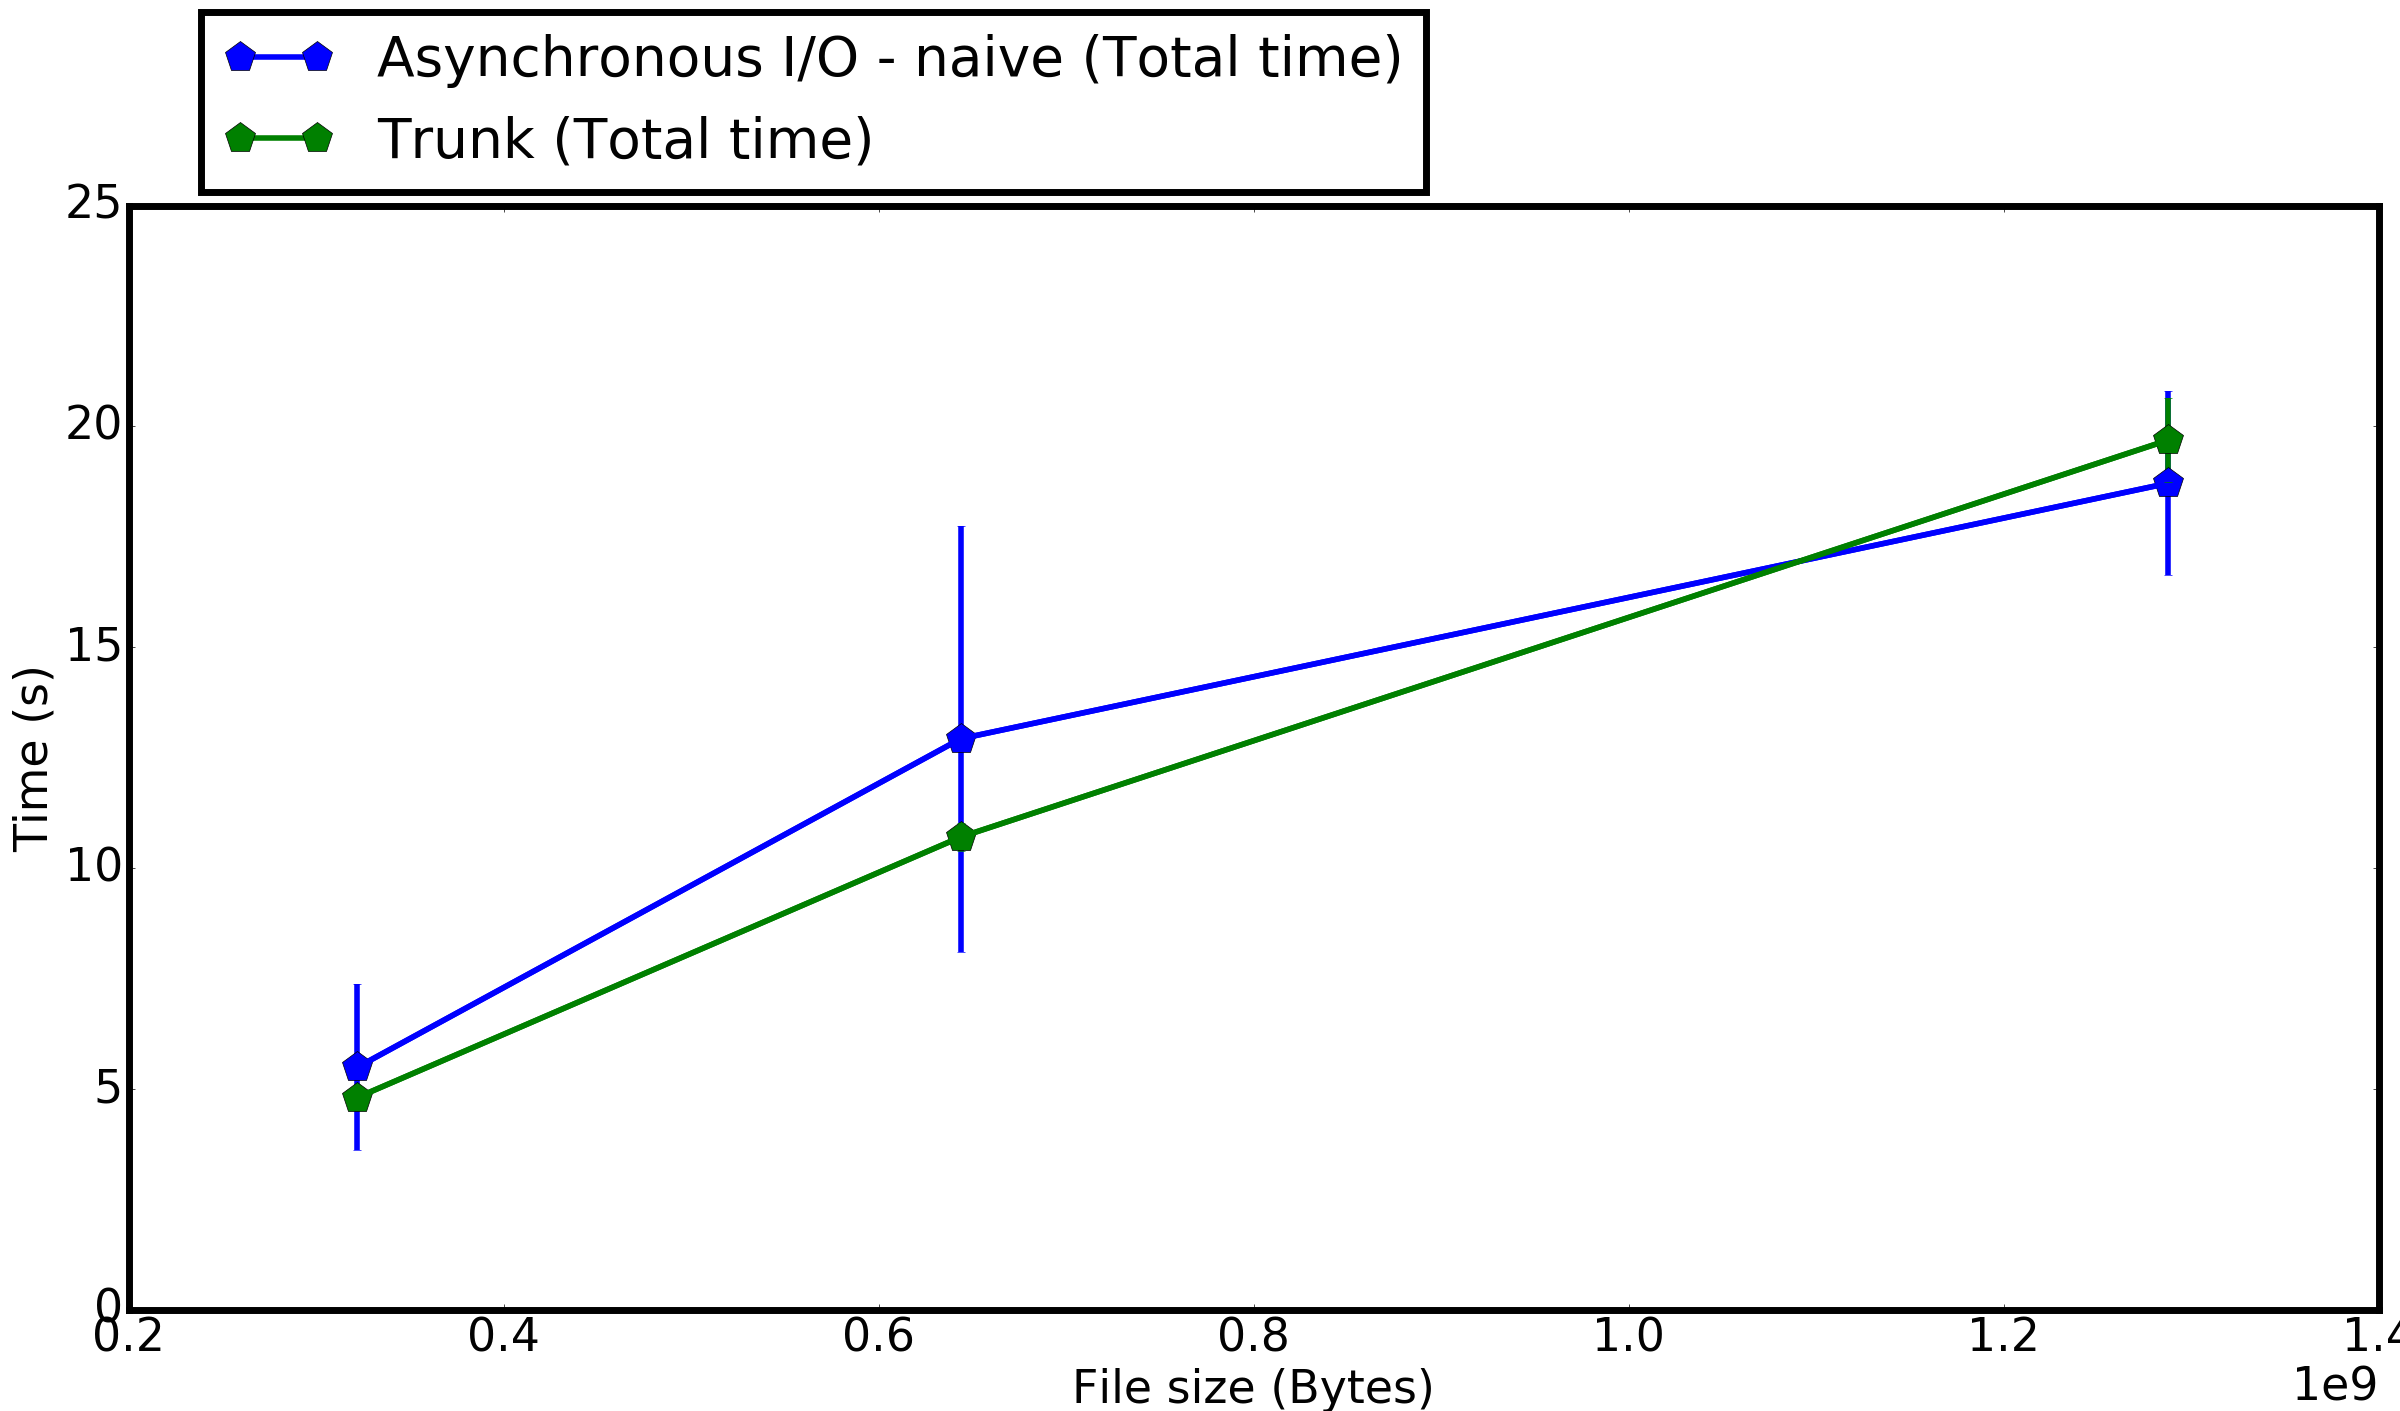
\includegraphics[width=\textwidth]{charts/cubeRemapper_basicImplementation_total_hpc.png}
					\caption[]%
					{{\small \targetPlatformHpc \space @ \targetPlatformHpcFrequency}}    
					\label{fig:cubeRemapper_basicImplementation_total_hpc}
				\end{subfigure}
				\caption{Experimental comparison of the \emph{compute} and \emph{total} time: proposed \emph{\notationaio\space} (naive) VS. \emph{state-of-the-art} (trunk synchronous) implementation of the \toolTargetSoftware}
				\label{fig:cubeRemapper_basicImplementation_compute_total}
			\end{figure*}

		However, the significant performance gain achieved in the \emph{write} operation is not transposed on the total time.   Indeed, Figures \ref{fig:cubeRemapper_basicImplementation_total_workstation_8core} and \ref{fig:cubeRemapper_basicImplementation_total_hpc} show that, on both considered platforms, the overall performance of our custom implementation is roughly comparable to that of the \emph{state-of-the-art}.   The gain achieved in the \emph{write} operation is lost in the \emph{compute} operation\footnote{This performance is shown by Figure \ref{fig:cubeRemapper_basicImplementation_compute_total}}.   More concerning is the \emph{compute} operation in our implementation.   Its value fluctuates within a range from $40$ to $80\%$.   Moreover, although our custom version and the state-of-the-art version use the same \emph{compute} function, we obtain a different response-time when this function is shipped to our implementation of the \toolTargetSoftware.\\


	\subsection{Improving the asynchronous-thread scheduling policy} \label{subsection:improveSchedulingPolicy}
		Based on our previous experimental observations, one could notice the interference between the \emph{compute} operation and our custom \emph{write} implementation.   Indeed, the \emph{compute} operation becomes less efficient once shipped to our version of the \toolTargetSoftware\space (despite the fact that it is the same implementations).\\
		Given the instability of this perturbation (see Figures \ref{fig:cubeRemapper_basicImplementation_compute_workstation_8core} and \ref{fig:cubeRemapper_basicImplementation_compute_hpc}), our first hypothesis to explain this phenomenon is related to the OS-scheduler policy.\\

		As all the considered threads (those processing the \emph{compute} and the \emph{write} operations) belong to the same process, the OS scheduler will tend to run them on the same CPU-core as often as possible (for cache proximity purpose).   Thus, the execution time of the \notationaioComputeThread\space is time-sliced and regularly interrupted for the execution of the \notationaioWriteThreads, most likely on the same CPU-core.   This may explain the delay observed on the experimental assessment of the compute \emph{operation} in our custom implementation (see Figures \ref{fig:cubeRemapper_basicImplementation_compute_workstation_8core} and \ref{fig:cubeRemapper_basicImplementation_compute_hpc}).\\

		Our solution to this resource-multiplexing issue is to pin each running thread on an independent CPU-core.   Assuming that our implementation has a relatively reduced amount of shared data and instructions between these threads (see Section \ref{subsection:dataDistribution}) then, having threads running on independent cores would significantly improve the parallelization with a reduced time overhead\footnote{Minimal shared data is equivalent to minimal synchronization required}.\\
		In order to pin the threads created by the \notationaio\space library, we have used the custom wrapper of the \emph{pthread} library described in Section \ref{subsubsection:pthreadWrapper}.\\

			\begin{figure*}[!h]
				\centering
				\begin{subfigure}[b]{0.475\textwidth}
					\centering
					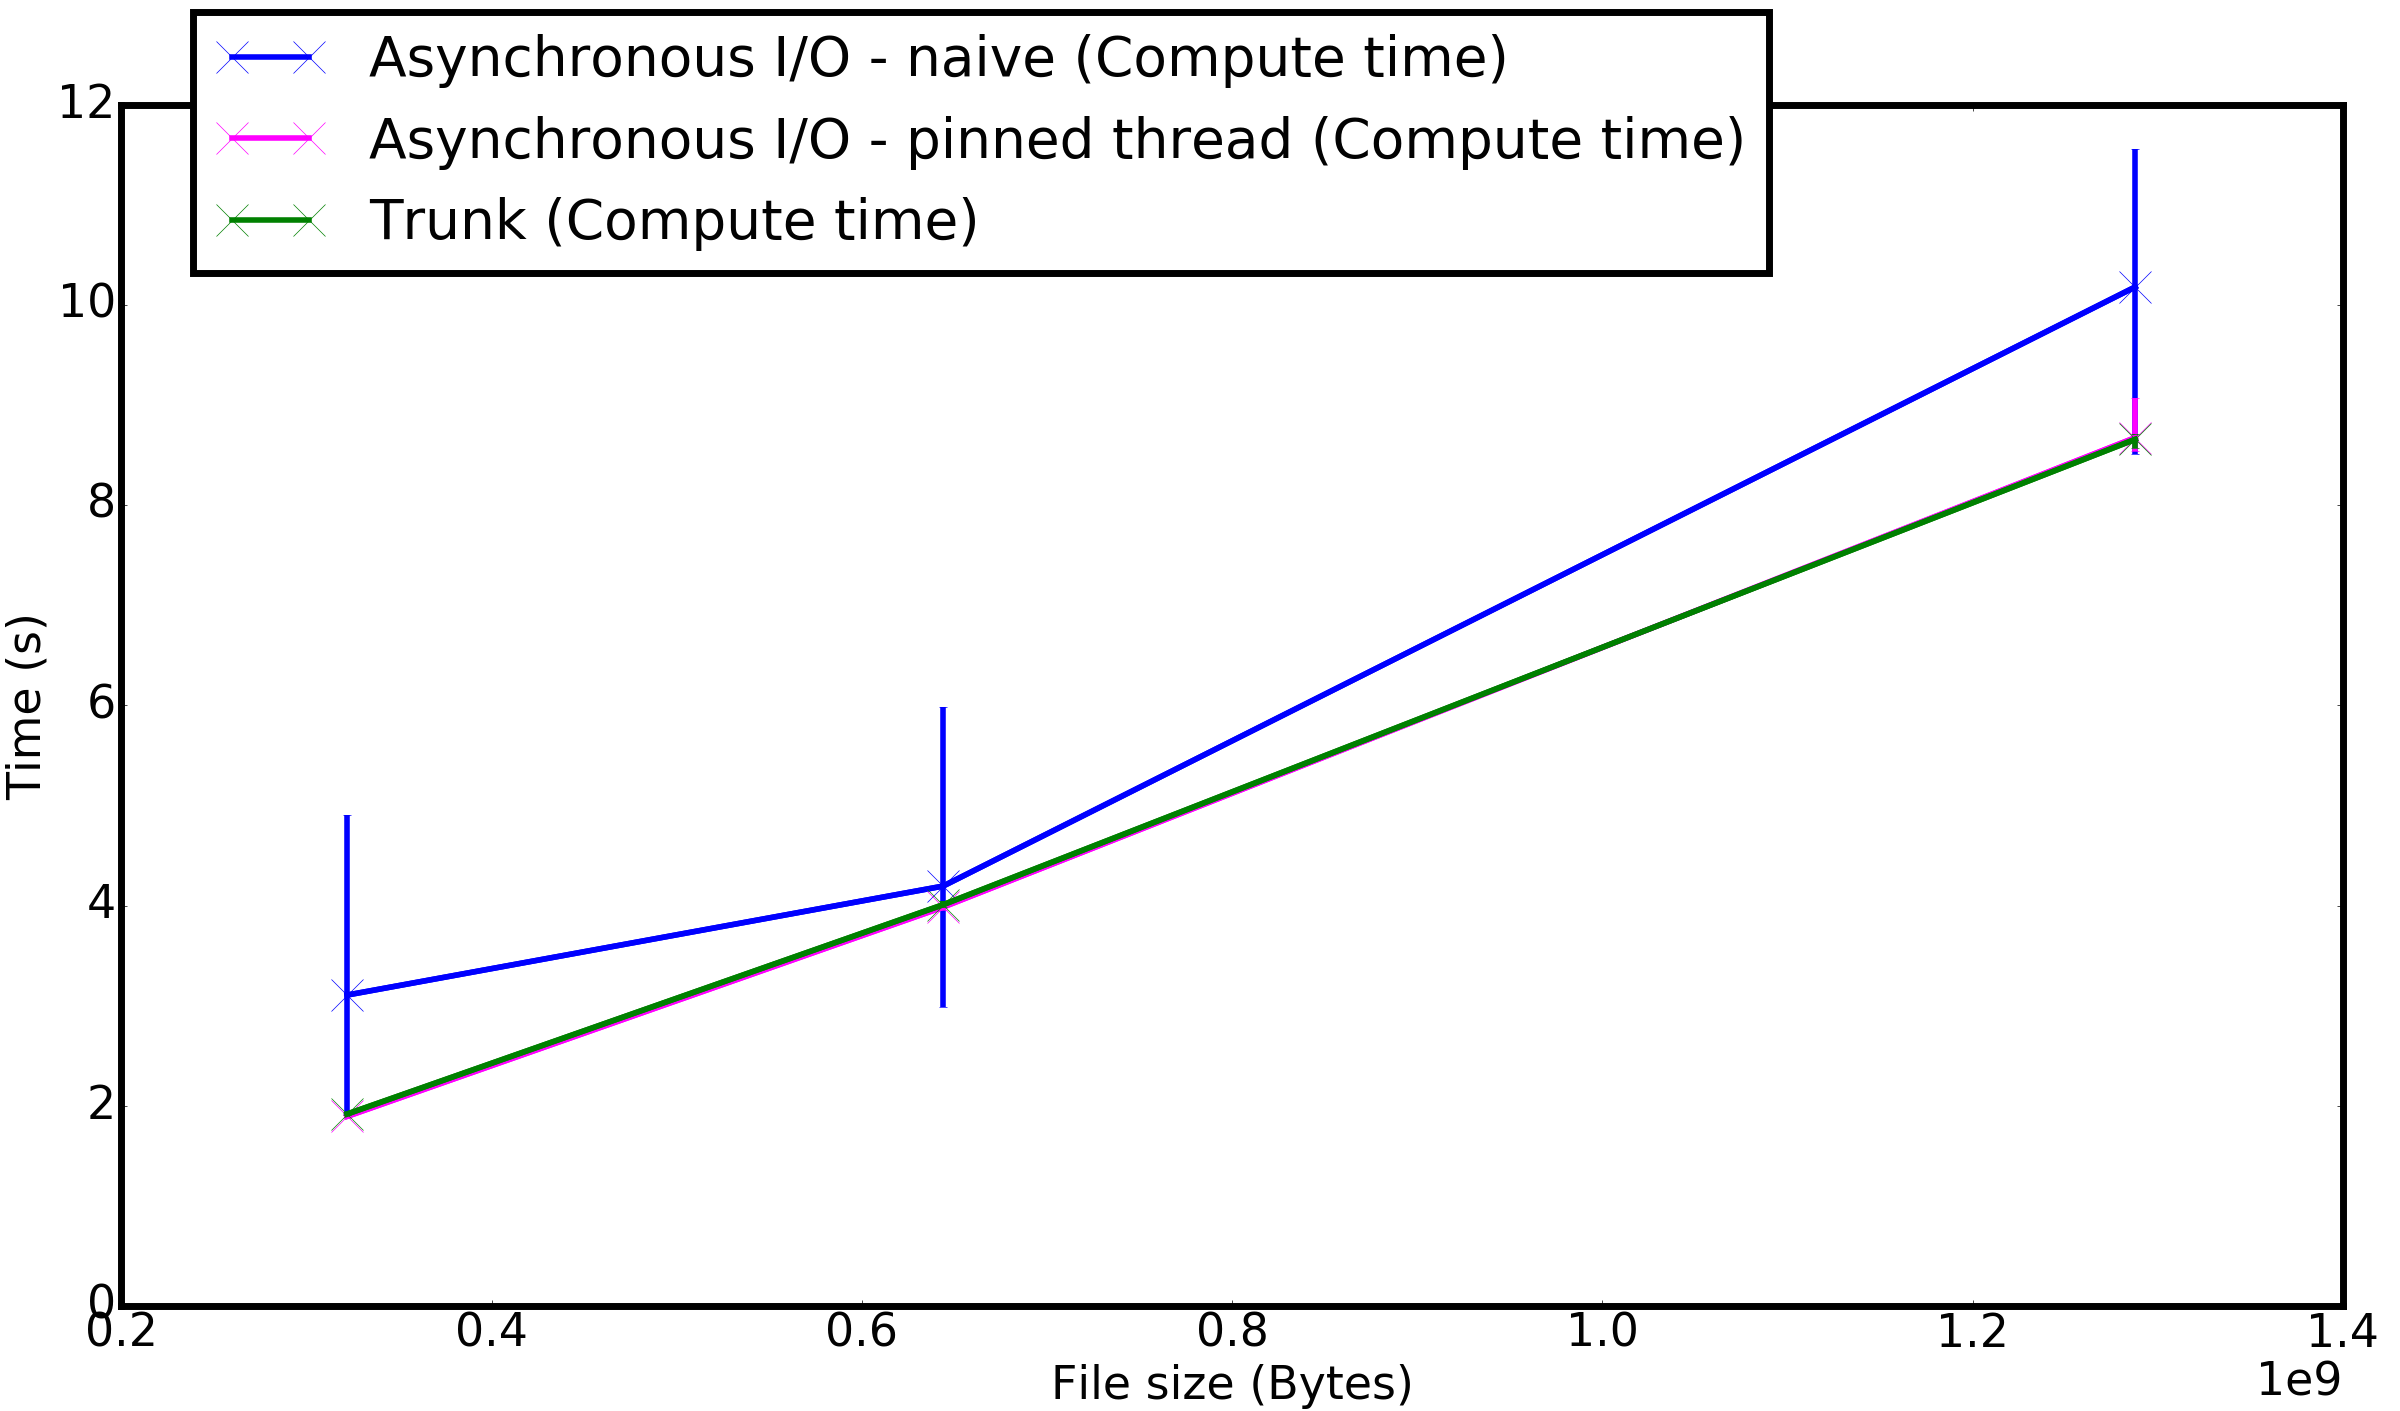
\includegraphics[width=\textwidth]{charts/cubeRemapper_pthreadWrap_compute_workstation_8core.png}
					\caption[\targetPlatformLaptop \space @ \targetPlatformLaptopFrequency]
					{{\small \targetPlatformLaptop \space @ \targetPlatformLaptopFrequency}}
					\label{fig:cubeRemapper_pthreadWrap_compute_workstation}
				\end{subfigure}
				\hfill
				\begin{subfigure}[b]{0.475\textwidth}
					\centering
					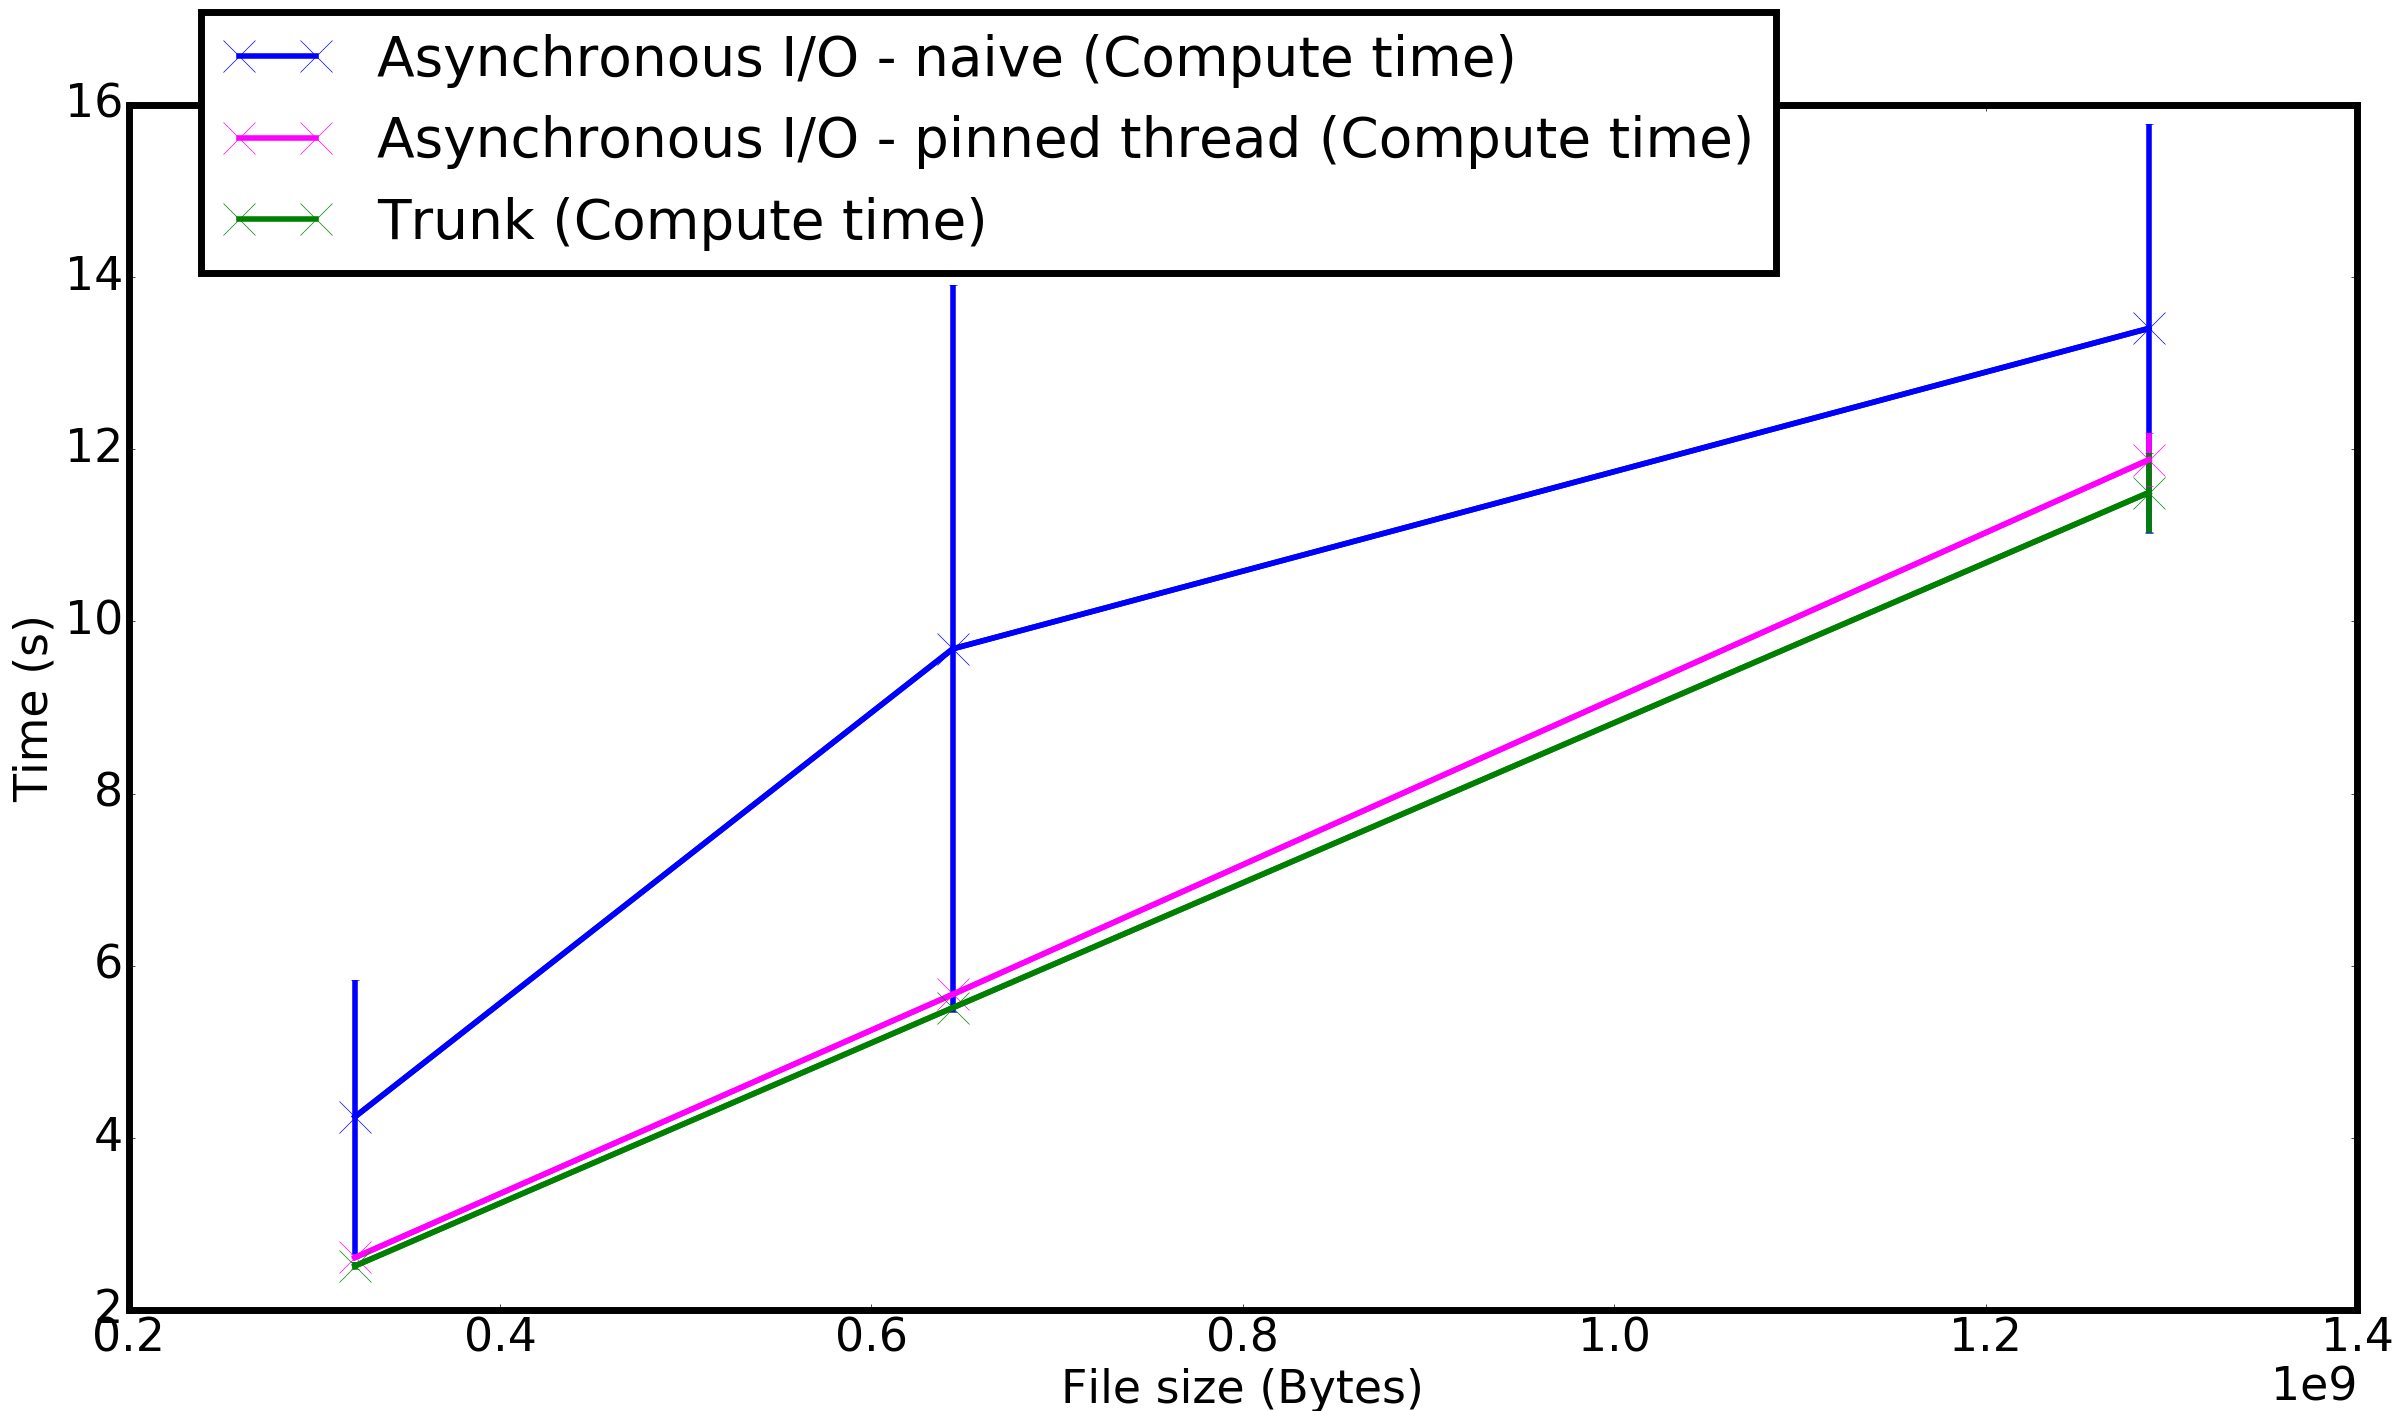
\includegraphics[width=\textwidth]{charts/cubeRemapper_pthreadWrap_compute_hpc.png}
					\caption[]%
					{{\small \targetPlatformHpc \space @ \targetPlatformHpcFrequency}}
					\label{fig:cubeRemapper_pthreadWrap_compute_hpc}
				\end{subfigure}
				\vskip\baselineskip
				\begin{subfigure}[b]{0.475\textwidth}
					\centering
					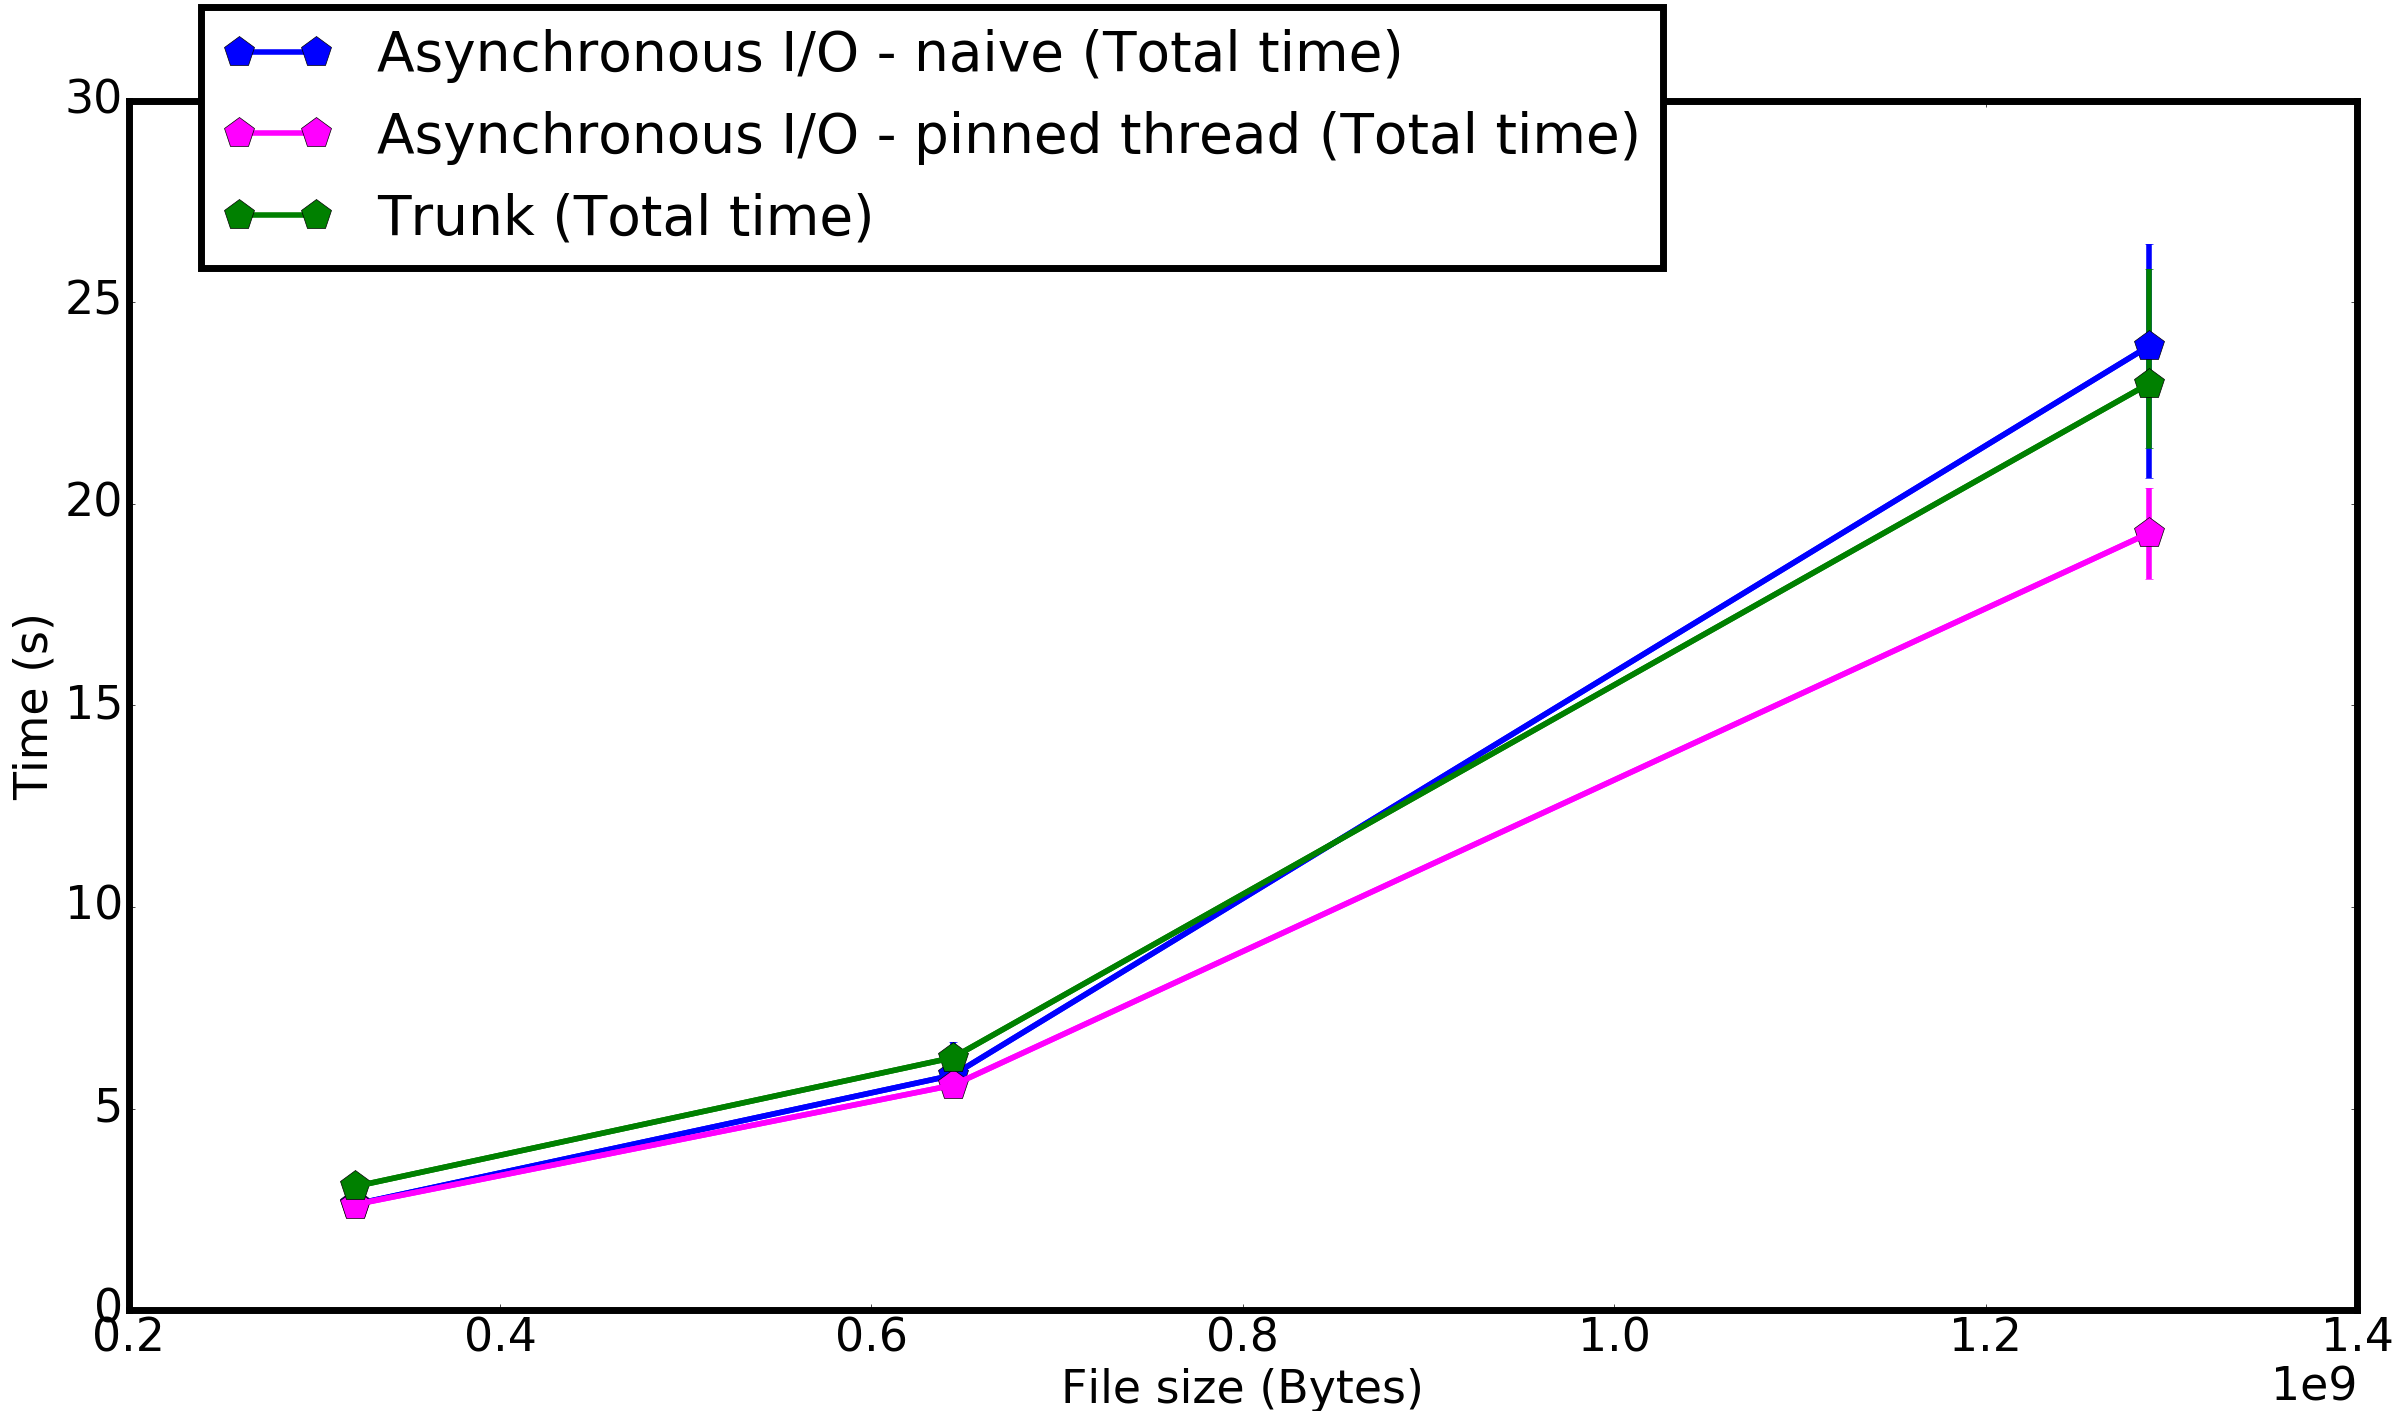
\includegraphics[width=\textwidth]{charts/cubeRemapper_pthreadWrap_total_workstation_8core.png}
					\caption[\targetPlatformLaptop \space @ \targetPlatformLaptopFrequency]
					{{\small \targetPlatformLaptop \space @ \targetPlatformLaptopFrequency}}
					\label{fig:cubeRemapper_pthreadWrap_total_workstation}
				\end{subfigure}
				\hfill
				\begin{subfigure}[b]{0.475\textwidth}
					\centering
					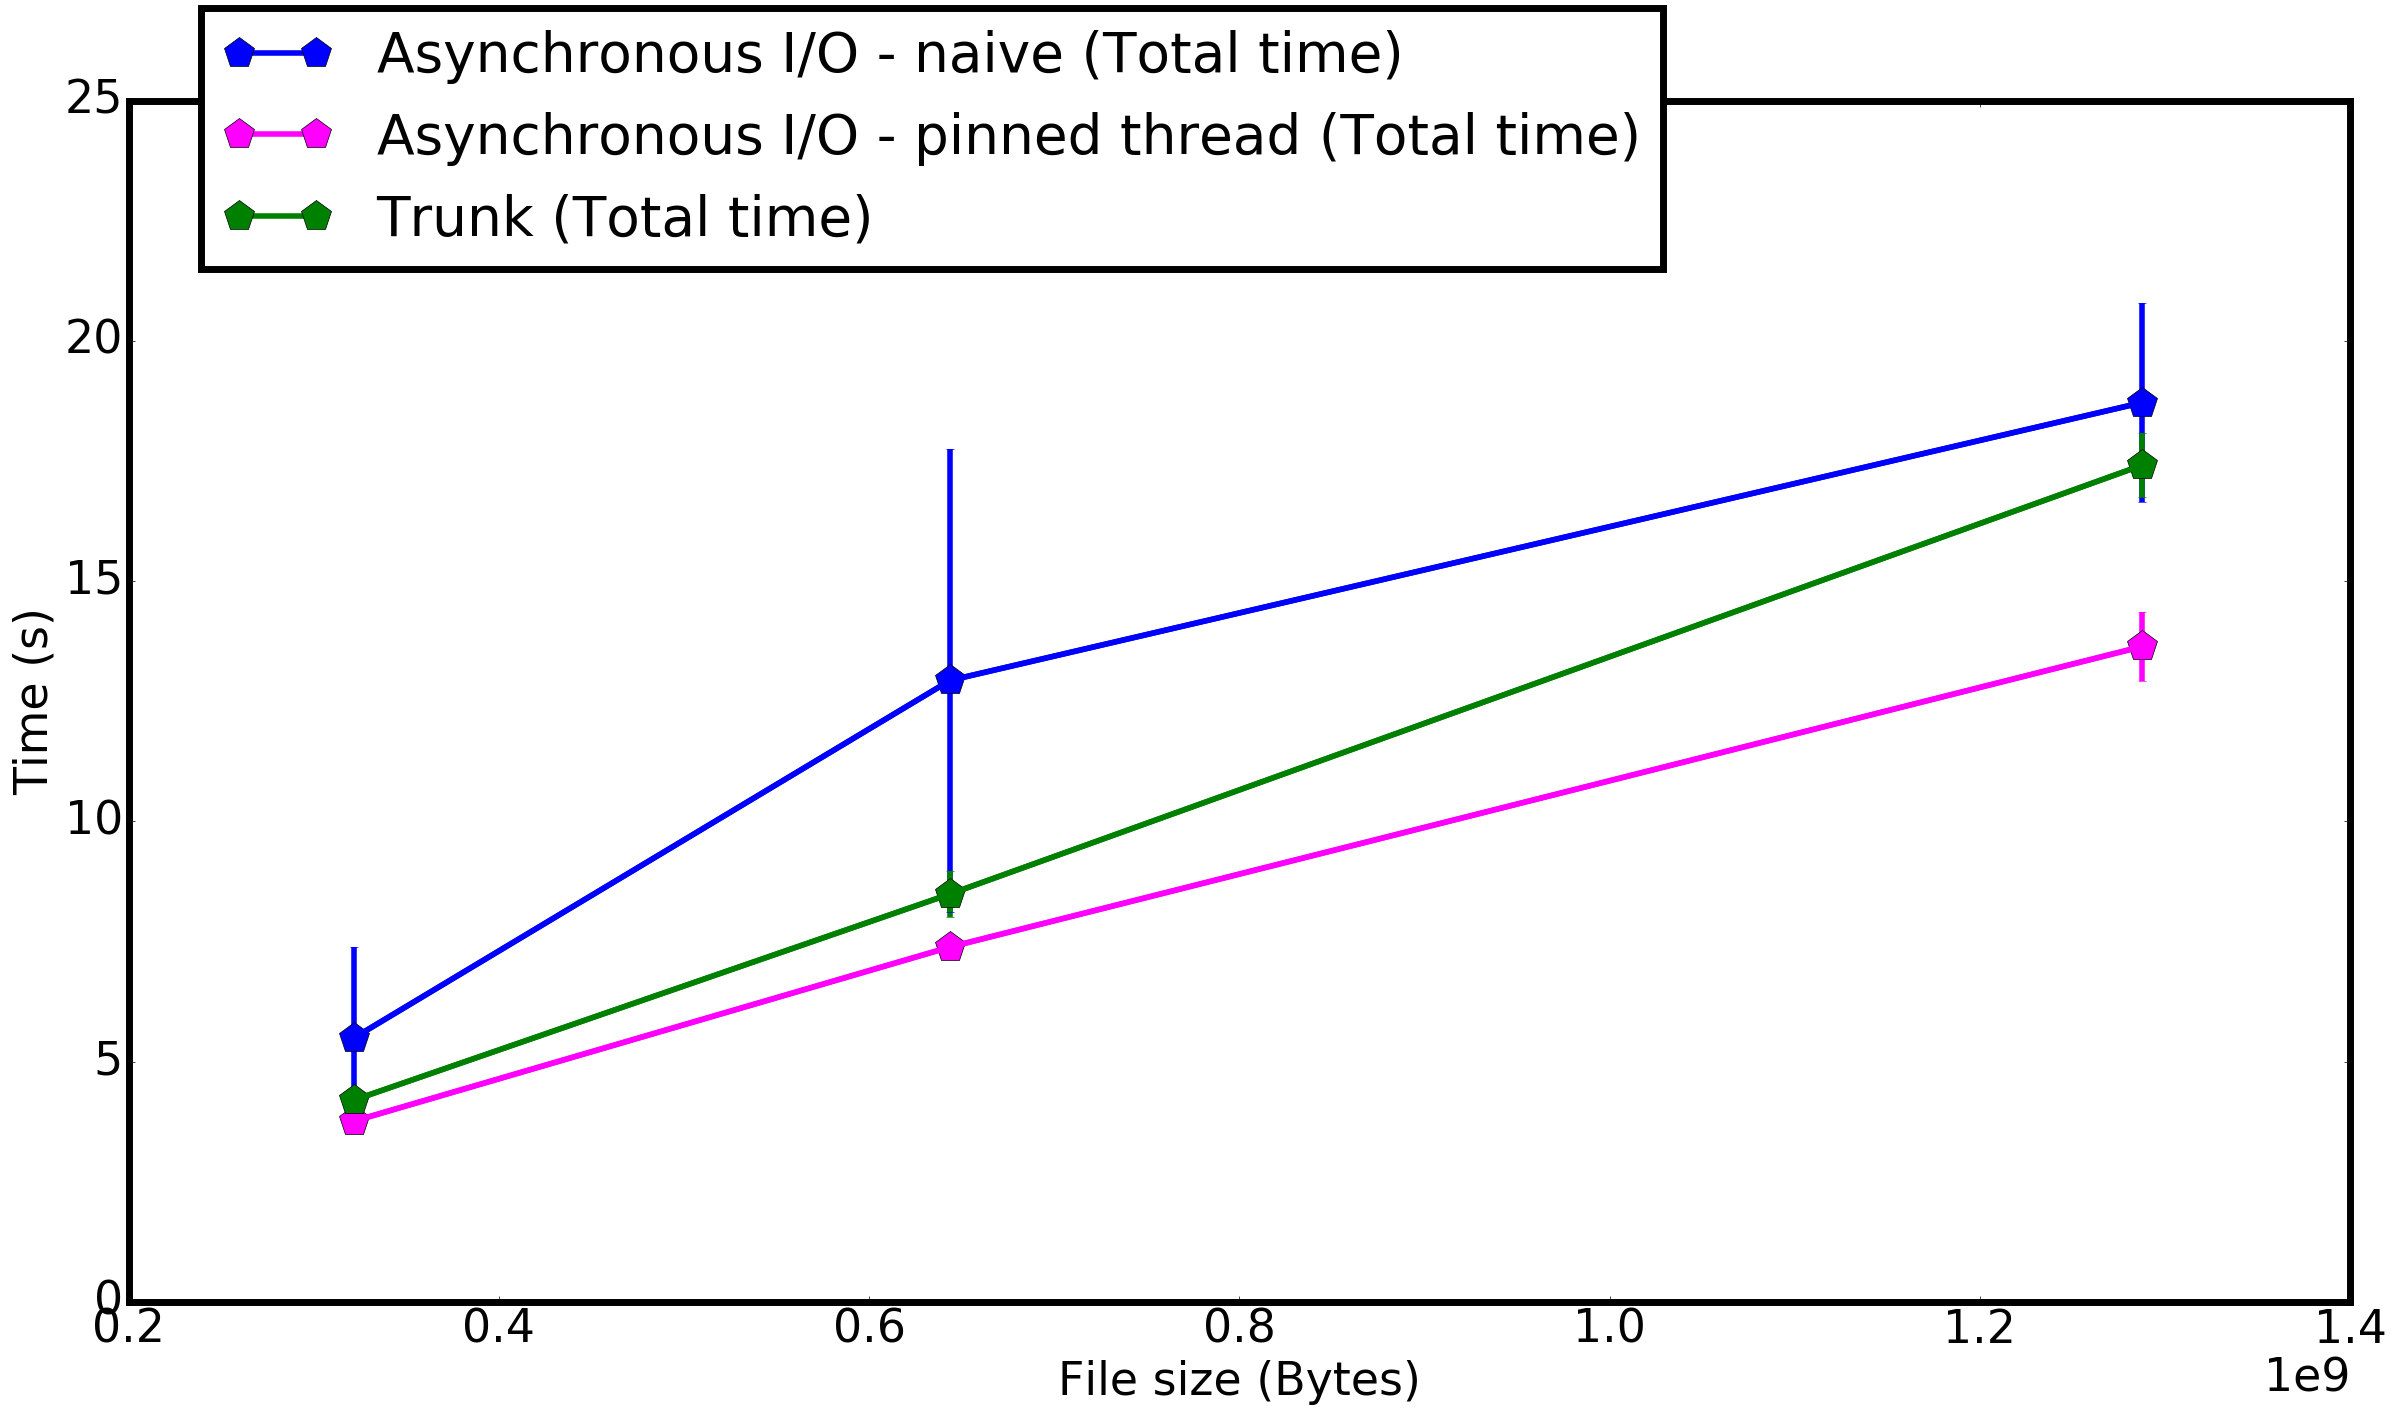
\includegraphics[width=\textwidth]{charts/cubeRemapper_pthreadWrap_total_hpc.png}
					\caption[]%
					{{\small \targetPlatformHpc \space @ \targetPlatformHpcFrequency}}
					\label{fig:cubeRemapper_pthreadWrap_total_hpc}
				\end{subfigure}
				\caption{Experimental comparison of the \emph{compute} and \emph{total} time: proposed \emph{\notationaio}\space (\emph{pinned thread}) VS. proposed \emph{\notationaio}\space (naive) VS. \emph{state-of-the-art} (trunk synchronous) implementation of the \toolTargetSoftware}
				\label{fig:cubeRemapper_pthreadWrap}
			\end{figure*}

		Figure \ref{fig:cubeRemapper_pthreadWrap} shows the impact of setting the thread affinity on the \emph{compute} operation in our custom implementation.   Indeed, Figures \ref{fig:cubeRemapper_pthreadWrap_compute_workstation} and \ref{fig:cubeRemapper_pthreadWrap_compute_hpc} show that the gap between the response time of the \emph{compute} operation in our enhanced custom implementation and the state-of-the-art one has been decreased to respectively $5$ and $2\%$ (compared to that of Figures \ref{fig:cubeRemapper_basicImplementation_compute_workstation_8core} and \ref{fig:cubeRemapper_basicImplementation_compute_hpc}) on the \targetPlatformHpc and the \targetPlatformLaptop platforms.\\
		Likewise, the size of the fluctuation of this operation has significantly collapsed (compared to that of Figure \ref{fig:cubeRemapper_basicImplementation_compute_workstation_8core} and \ref{fig:cubeRemapper_basicImplementation_compute_hpc}).\\
		Consequently, the overall gain achieved by our enhanced asynchronous strategy is now clearly confirmed.   In Figures \ref{fig:cubeRemapper_pthreadWrap_total_workstation} and \ref{fig:cubeRemapper_pthreadWrap_total_hpc}, the total time of our implementation is about $60\%$  more efficient than that of the state-of-the-art.   Moreover, the error margin of the \emph{compute} operation has been dramatically reduced.   Thus, the observed overall improvement is now clearly achieved and in a more robust manner (regardless of the error margin).


	\subsection{Reducing the impact of false-sharing} \label{subsection:lightenFalseSharing}
		Despite our effort to reduce the number of shared memory addresses and reduce the impact of synchronization between threads, Figures \ref{fig:cubeRemapper_basicImplementation_compute_total} and \ref{fig:cubeRemapper_pthreadWrap} show that the overhead due to synchronization might still be reduced\footnote{The execution time of the \emph{compute} function in our implementation is still slightly higher than the one in the \emph{state-of-the-art} implementation}.   Given that we managed to use independent buffers between concurrent threads (RAM level), our explanation is that this interference is due to \emph{false-sharing} (cache level).\\

		In Figures \ref{fig:cubeRemapper_falseSharing_compute_L3_workstation_8core} and \ref{fig:cubeRemapper_falseSharing_compute_L3_hpc}, we have represented the cache access foot-print of each one of the \emph{state-of-the-art} (\emph{trunk}), the \emph{naive} and the \emph{aligned buffer} implementations of the \toolTargetSoftware.   As one can notice, the number of cache misses in the \emph{naive} version of the code is about $33\%$ higher than that of the \emph{state-of-the-art} one.   Given that these two curves profile the same implementation of the \emph{compute} function, this shows the impact of \emph{false-sharing} on our implementation.   This result is also correlated with the one at time level (Figure \ref{fig:cubeRemapper_falseSharing_compute_time_workstation_8core} and \ref{fig:cubeRemapper_falseSharing_compute_time_hpc}).\\

			\begin{figure*}[!h]
				\centering
				\begin{subfigure}[b]{0.475\textwidth}
					\centering
					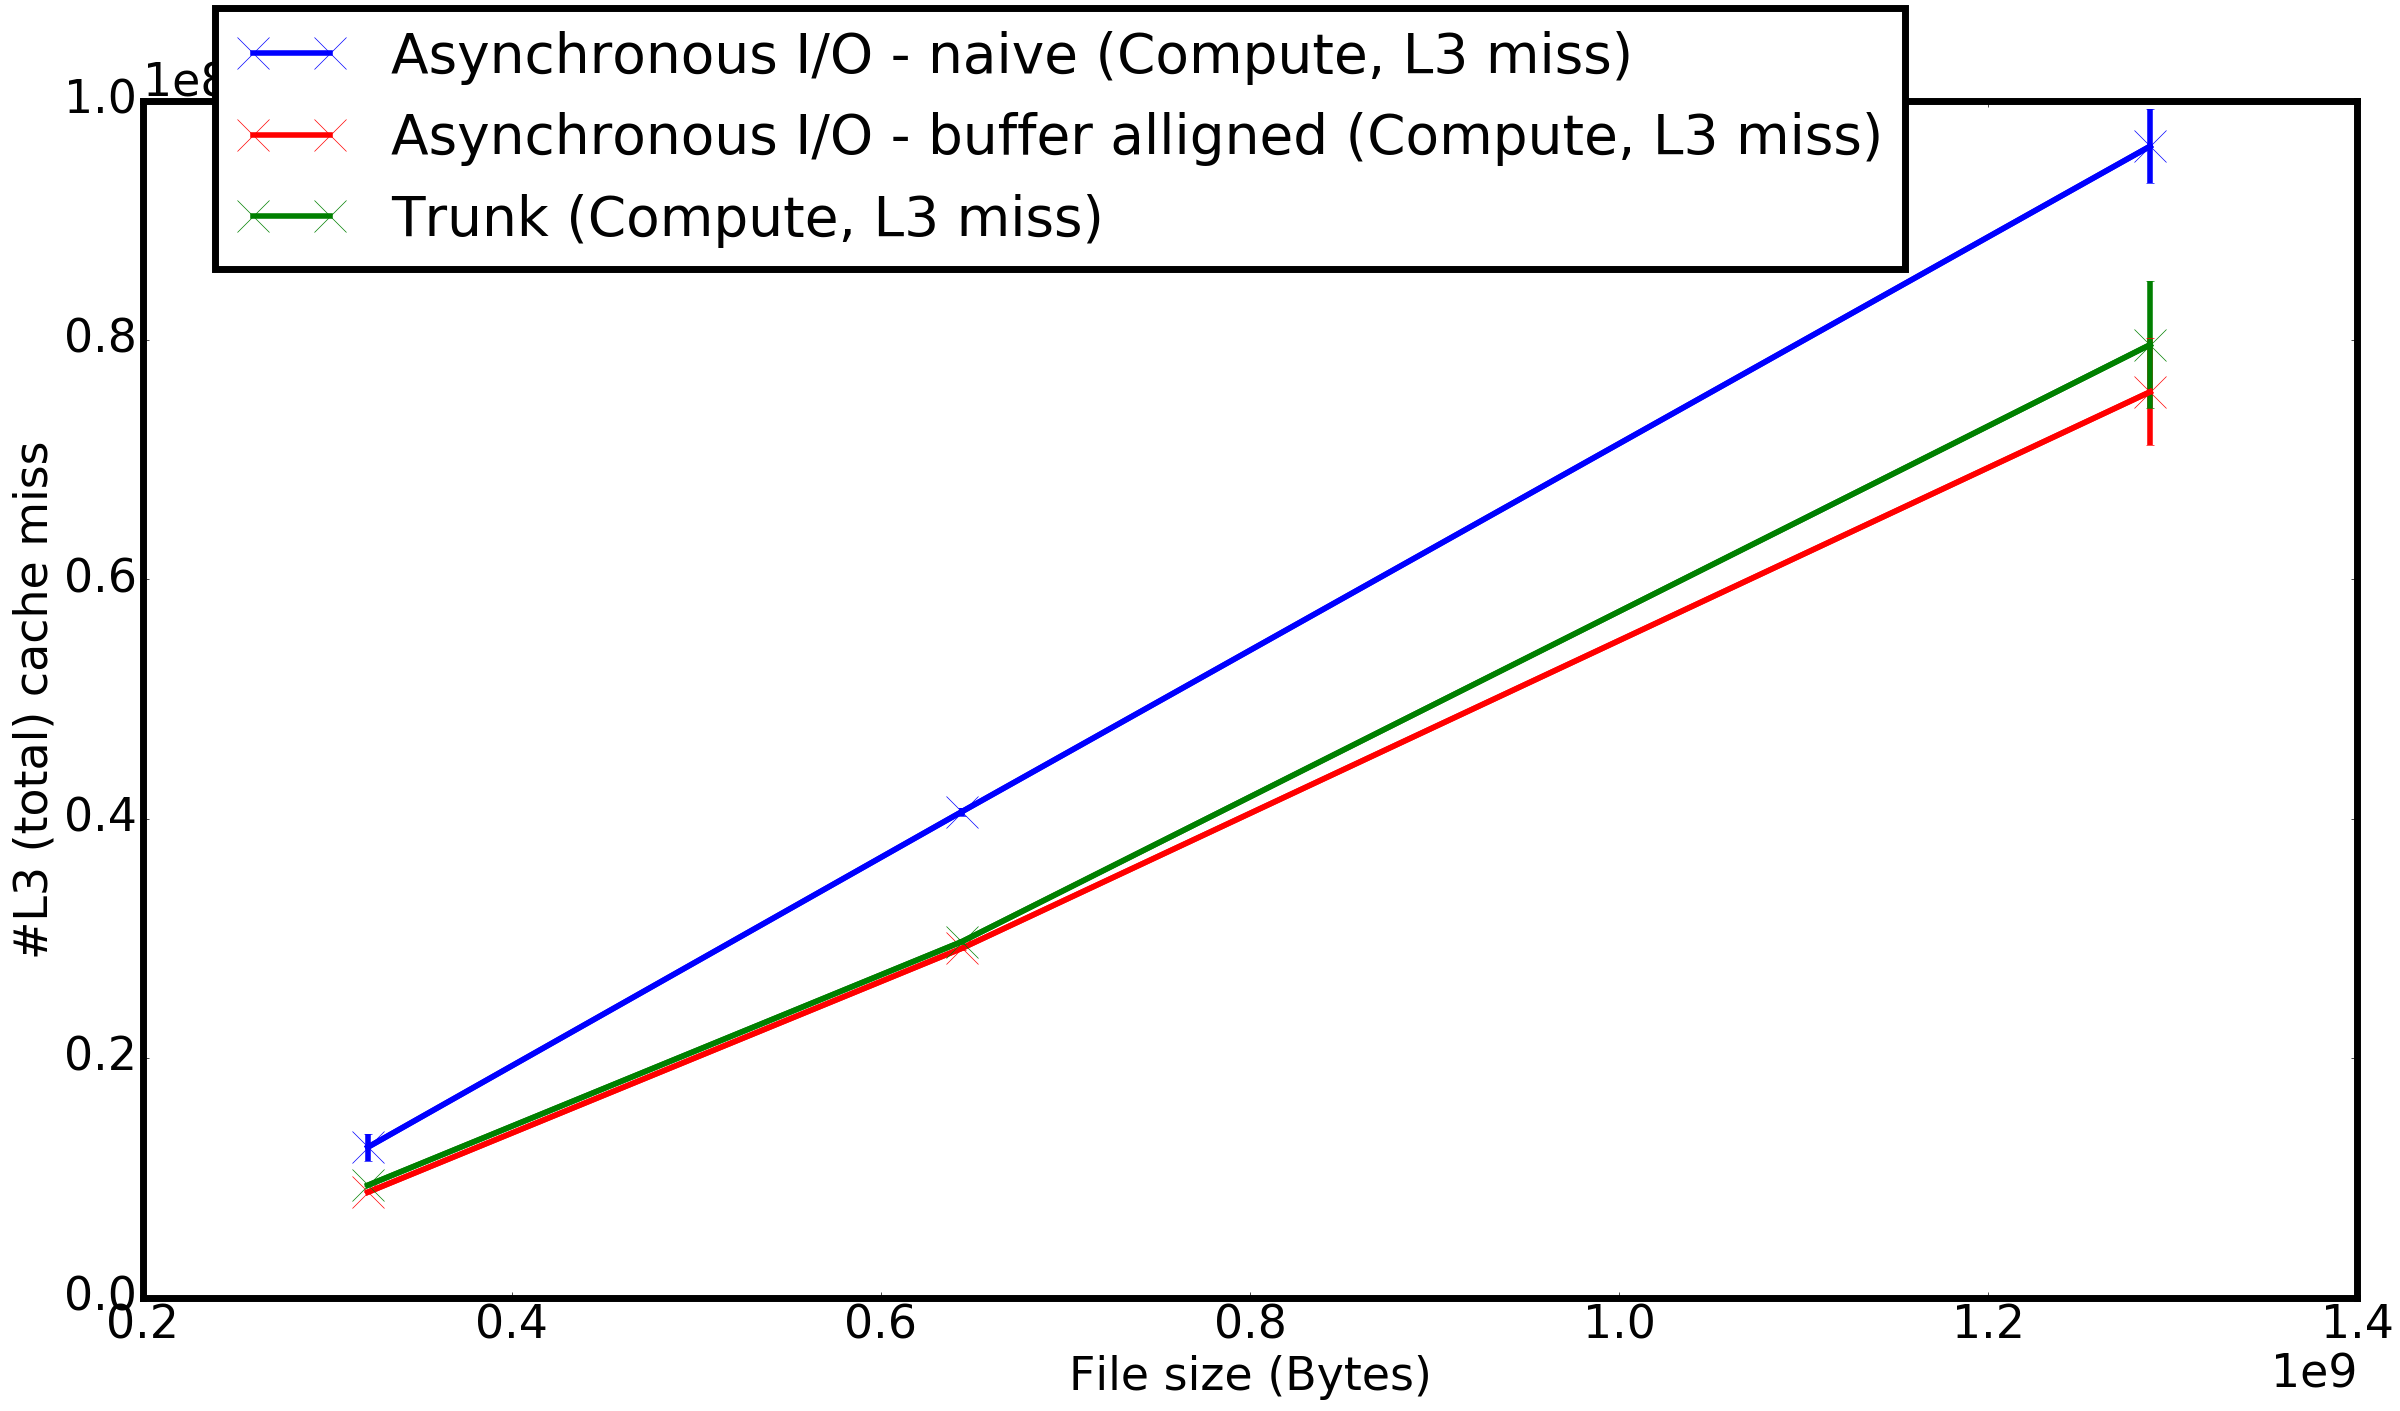
\includegraphics[width=\textwidth]{charts/cubeRemapper_falseSharing_compute_trackL3_workstation_8core.png}
					\caption[\targetPlatformLaptop \space @ \targetPlatformLaptopFrequency]
					{{\small \targetPlatformLaptop \space @ \targetPlatformLaptopFrequency}}
					\label{fig:cubeRemapper_falseSharing_compute_L3_workstation_8core}
				\end{subfigure}
				\hfill
				\begin{subfigure}[b]{0.475\textwidth}  
					\centering
					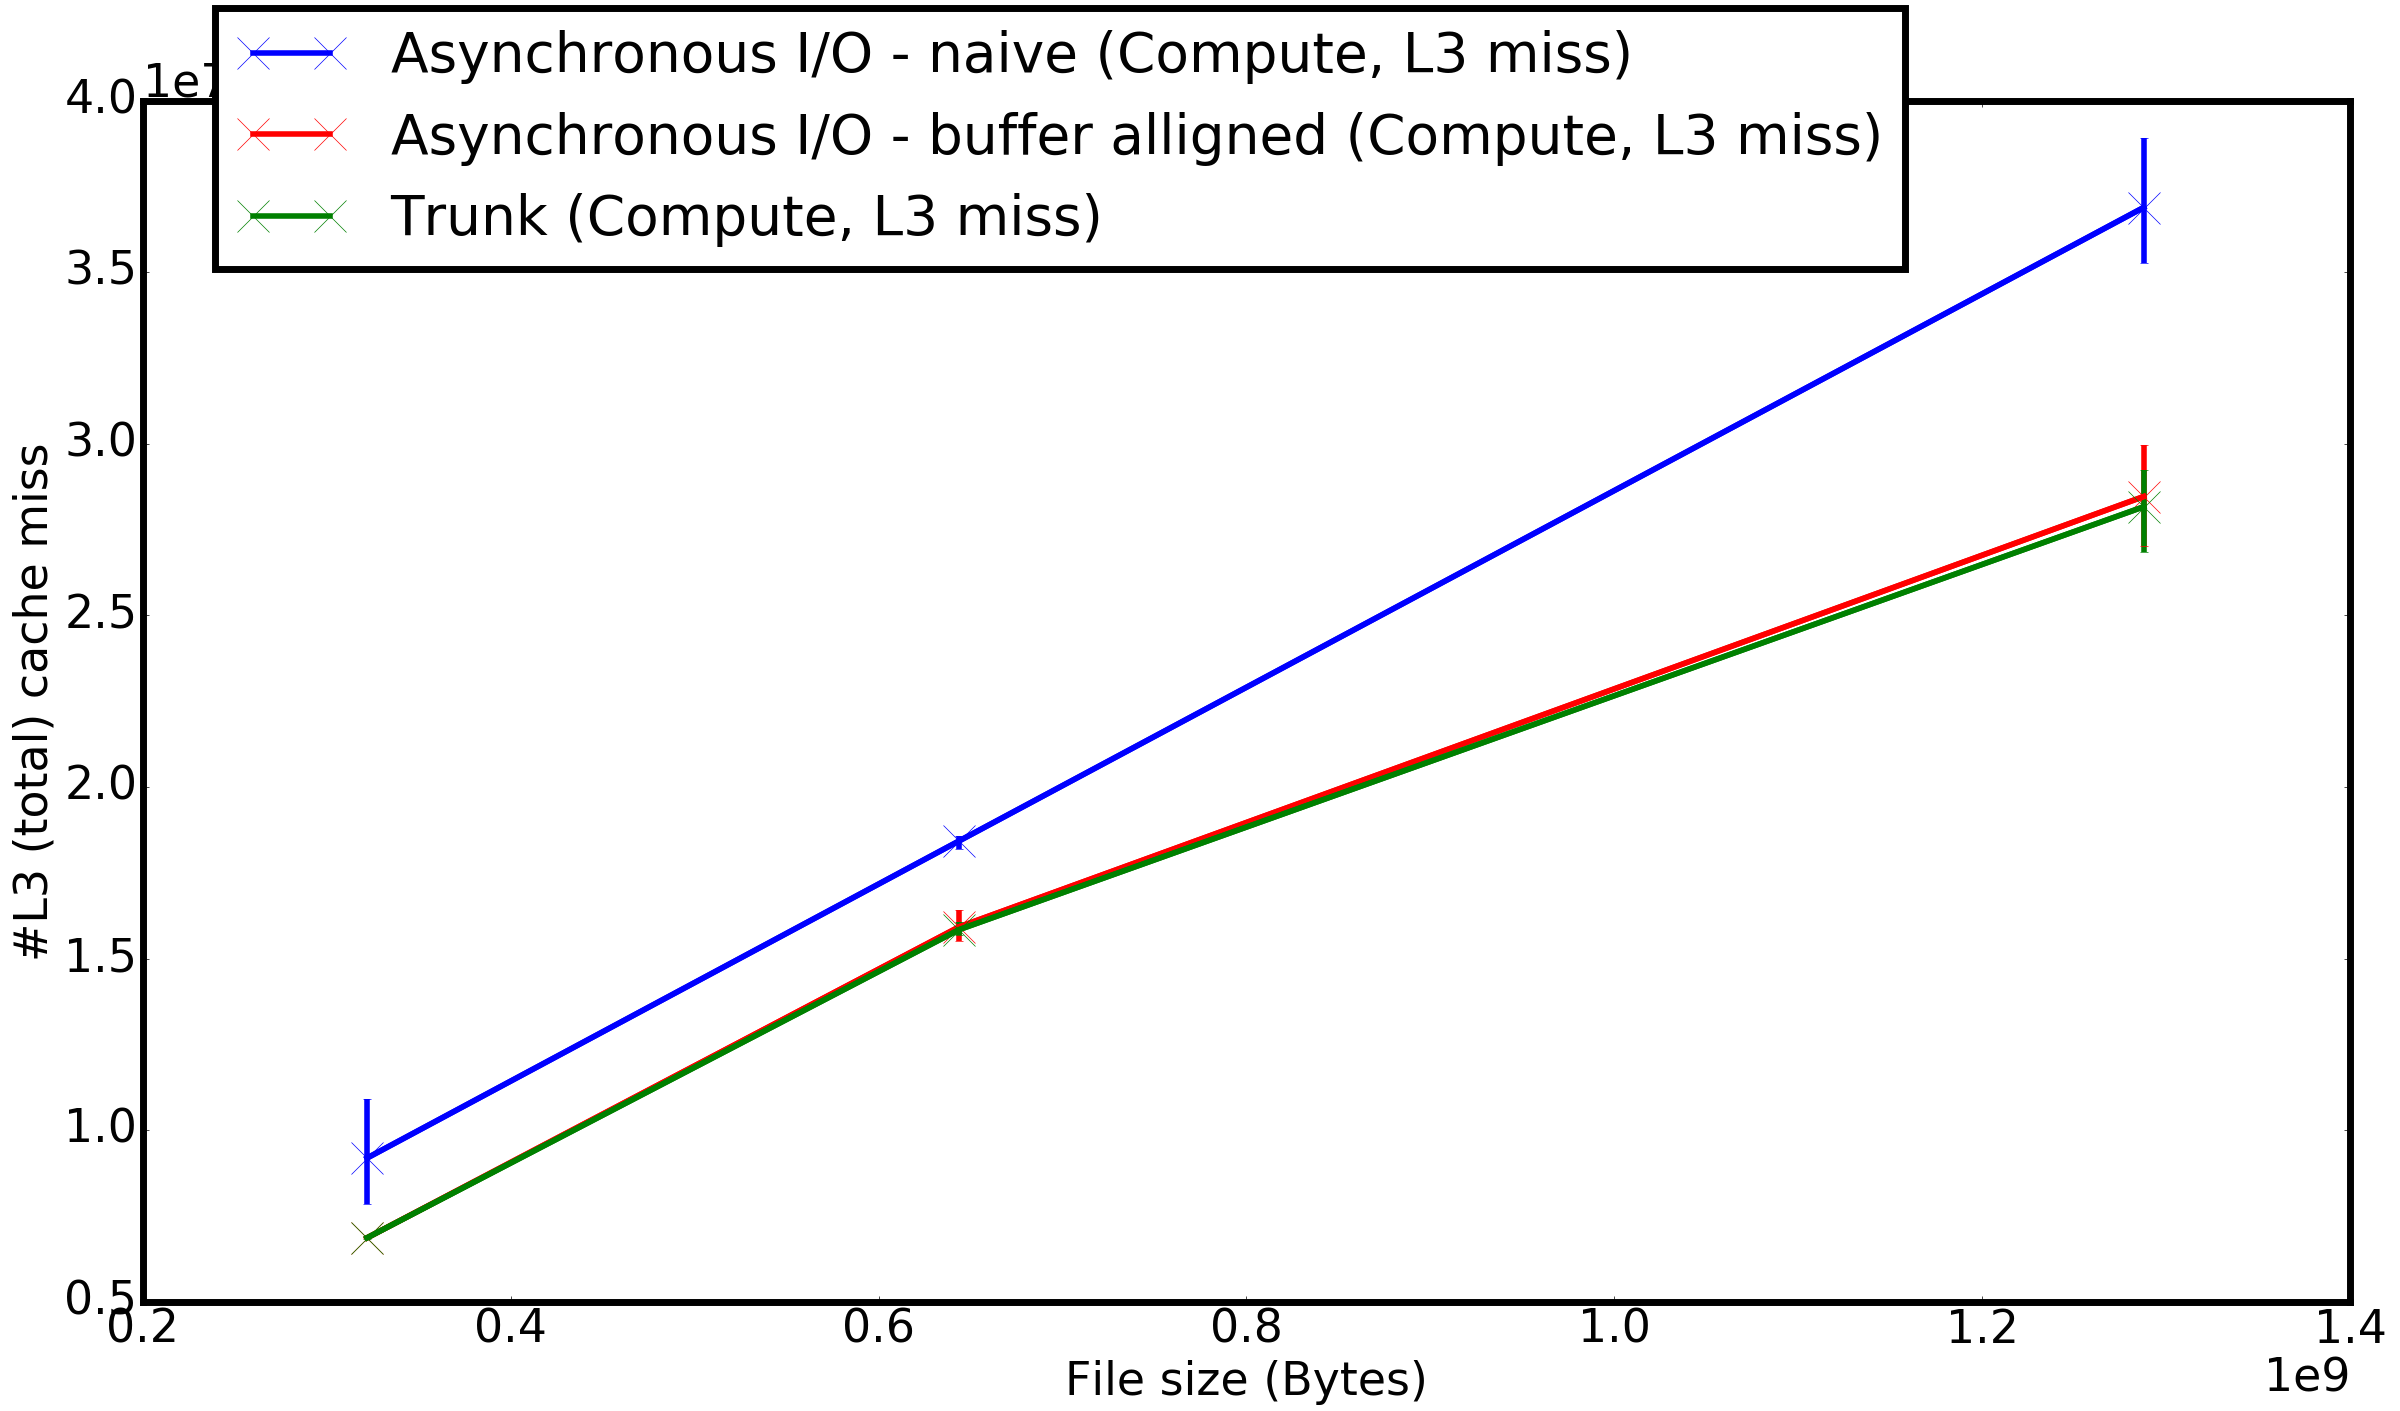
\includegraphics[width=\textwidth]{charts/cubeRemapper_falseSharing_compute_trackL3_hpc.png}
					\caption[]%
					{{\small \targetPlatformHpc \space @ \targetPlatformHpcFrequency}}
					\label{fig:cubeRemapper_falseSharing_compute_L3_hpc}
				\end{subfigure}
				\vskip\baselineskip
				\begin{subfigure}[b]{0.475\textwidth}
					\centering
					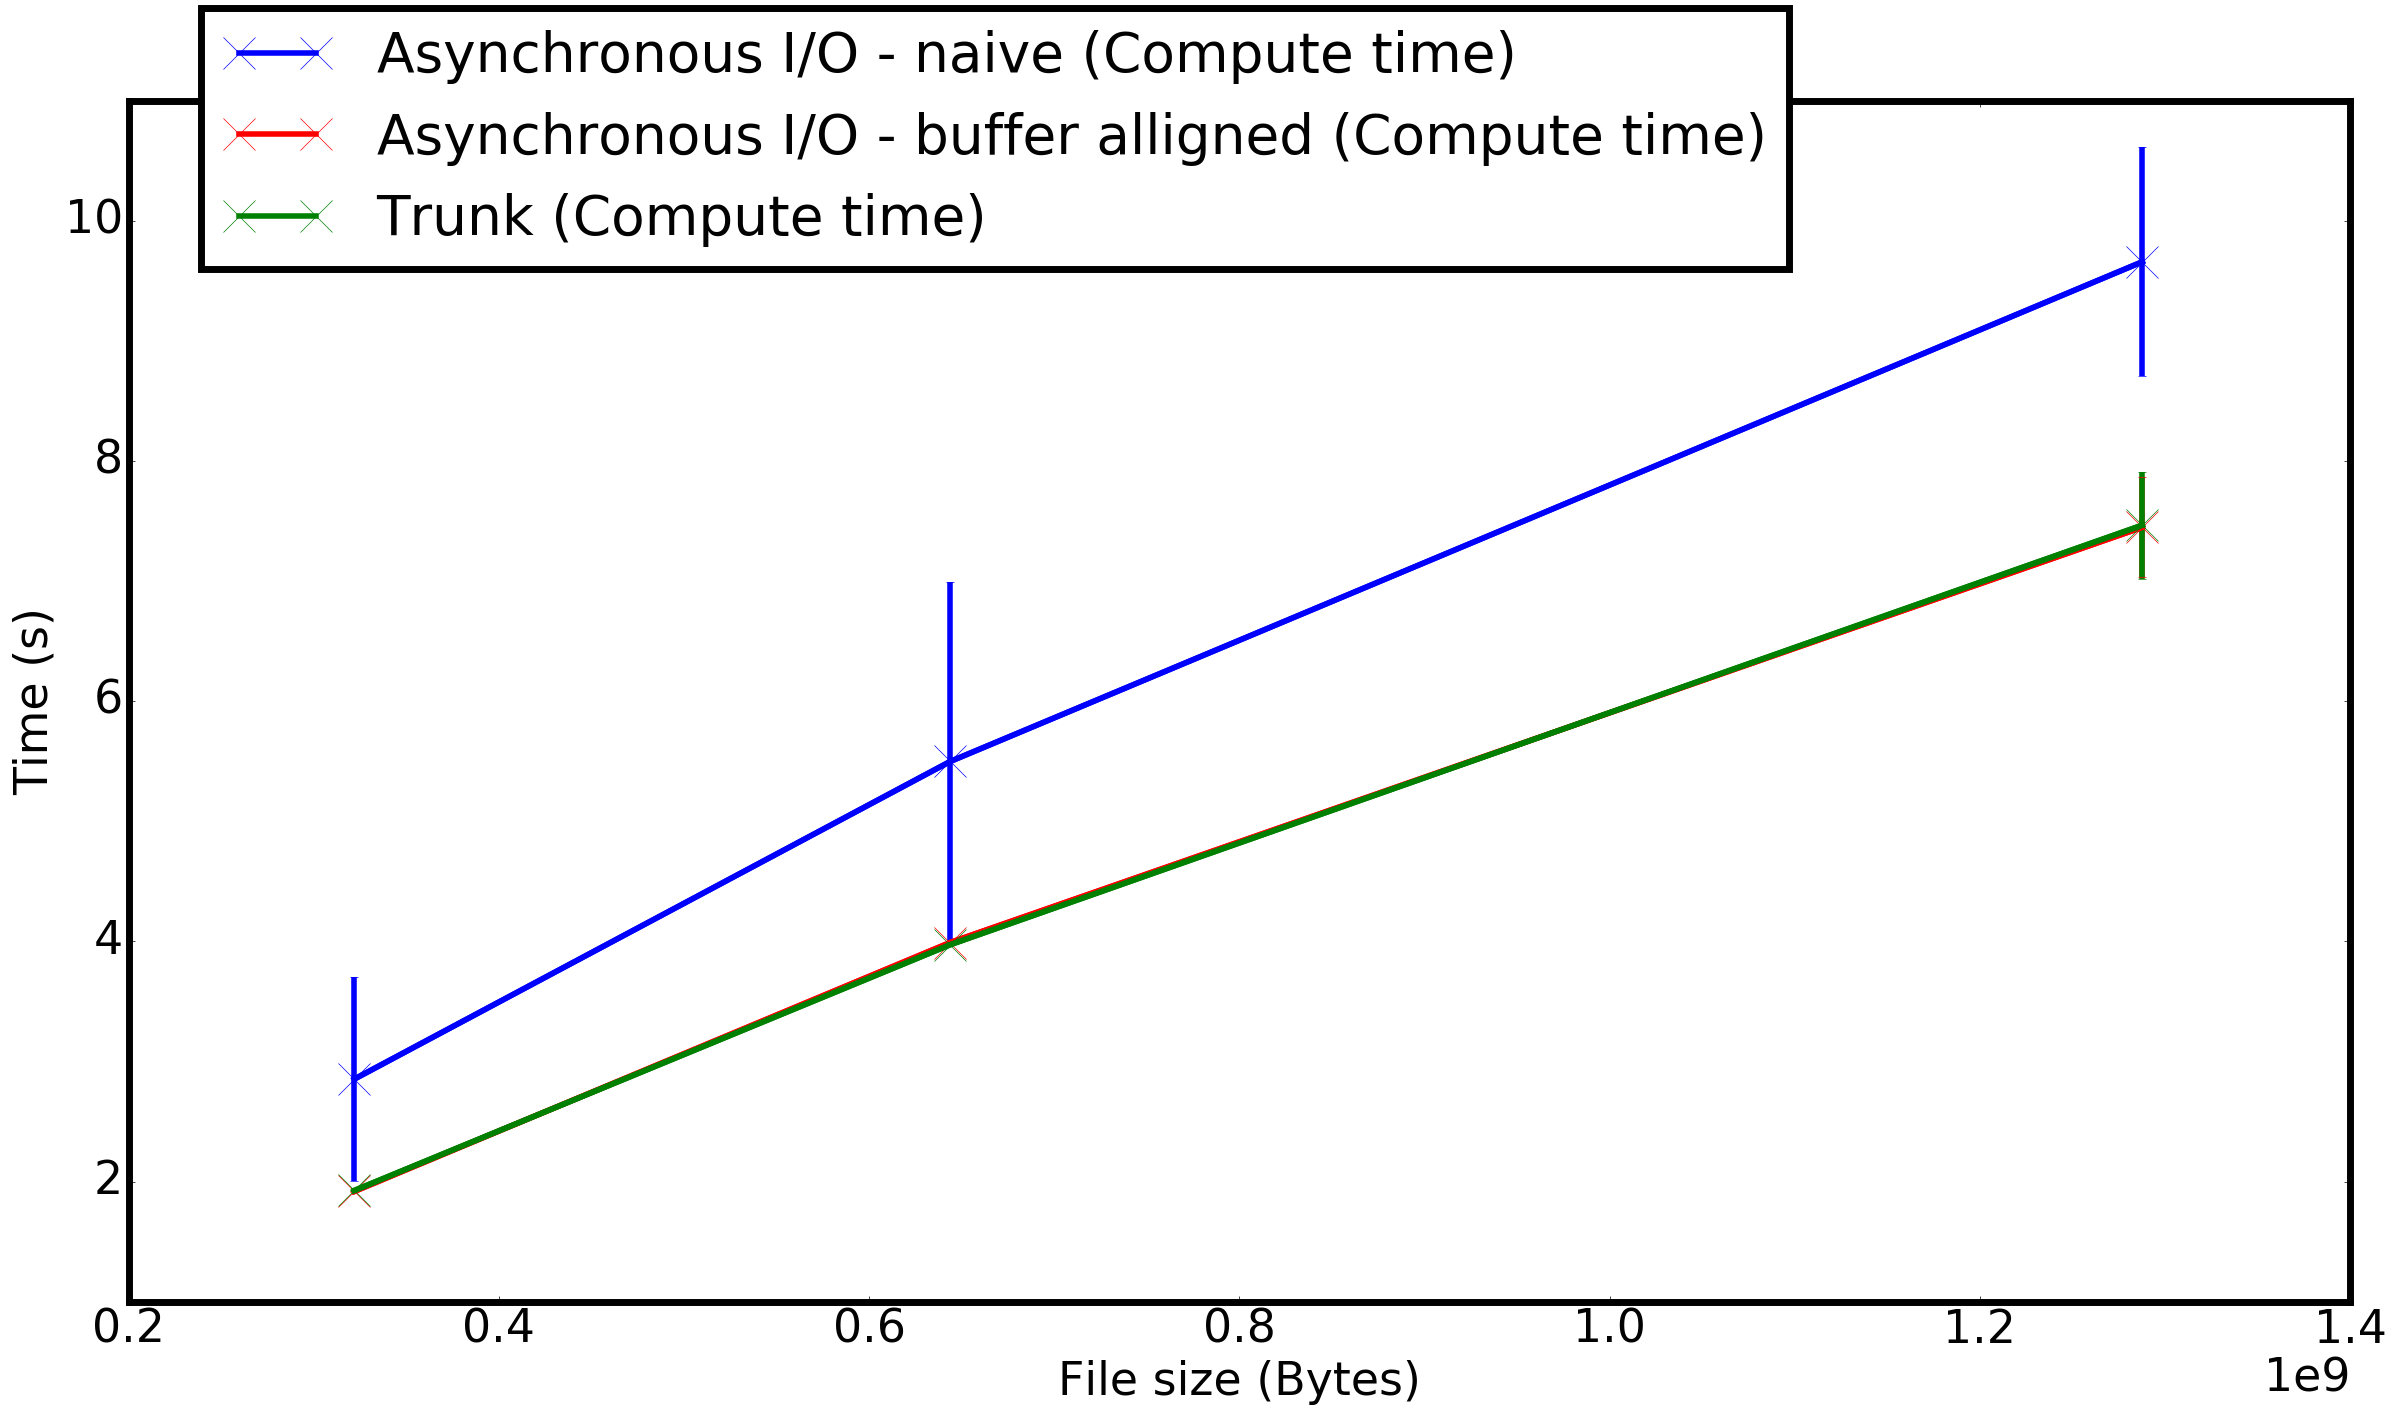
\includegraphics[width=\textwidth]{charts/cubeRemapper_falseSharing_compute_time_workstation_8core.png}
					\caption[]%
					{{\small \targetPlatformLaptop @ \targetPlatformLaptopFrequency}}
					\label{fig:cubeRemapper_falseSharing_compute_time_workstation_8core}
				\end{subfigure}
				\hfill
				\begin{subfigure}[b]{0.475\textwidth}  
					\centering 
					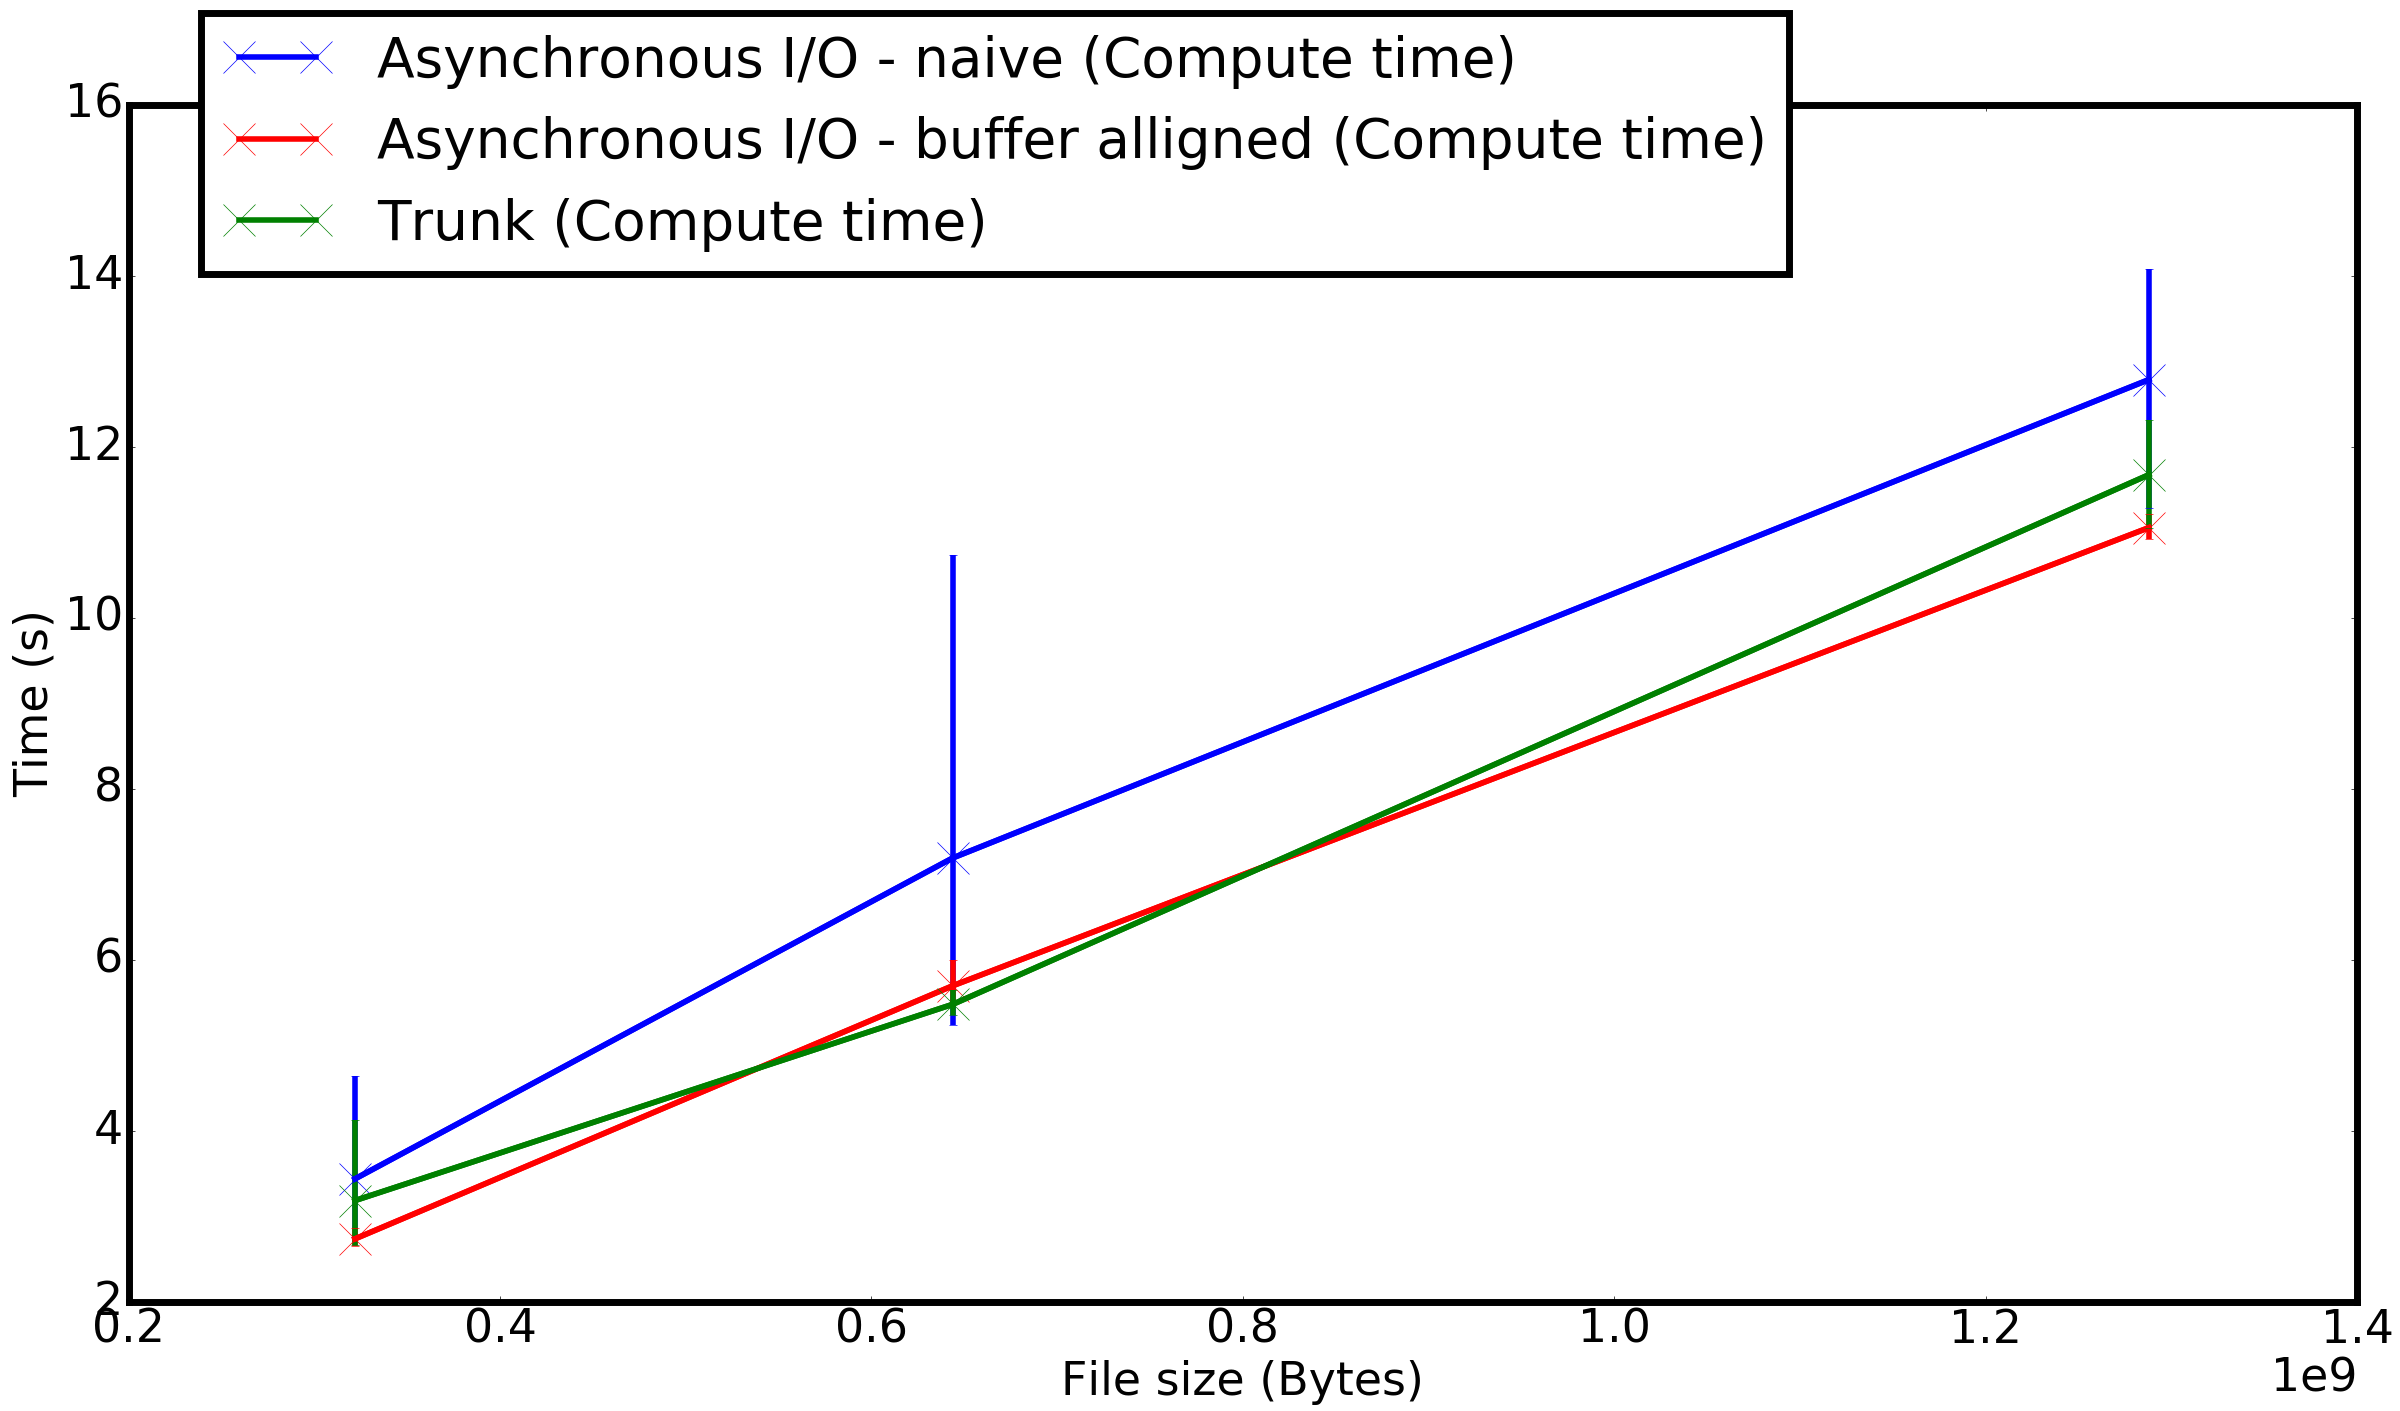
\includegraphics[width=\textwidth]{charts/cubeRemapper_falseSharing_compute_time_hpc.png}
					\caption[]%
					{{\small \targetPlatformHpc \space @ \targetPlatformHpcFrequency}}
					\label{fig:cubeRemapper_falseSharing_compute_time_hpc}
				\end{subfigure}
				\caption{Experimental comparison of the \emph{L3 cache-miss} (total) and \emph{compute} time: proposed \emph{\notationaio}\space (buffer aligned) VS. proposed \emph{\notationaio}\space (naive) VS. \emph{state-of-the-art} (trunk synchronous) implementation of the \toolTargetSoftware.   For the seek of clarity the only results represented are the one linked to the \emph{compute} operation}
				\label{fig:cubeRemapper_falseSharing_compute}
			\end{figure*}

		Furthermore, we see in Figures \ref{fig:cubeRemapper_falseSharing_compute_L3_workstation_8core} and \ref{fig:cubeRemapper_falseSharing_compute_L3_hpc} that the rate of cache misses in our \emph{buffer aligned} version drops down to the same level as that of the \emph{state-of-the-art} implementation.    Thus, our improvement allows to eliminate the cache-linked interferences between concurrent threads.\\
		This improvement, noticed at cache level, has a clear impact on the overall performance of our implementation.   Indeed, we observe in Figure \ref{fig:cubeRemapper_falseSharing_overall_time} an average gain of $70\%$ of the total time.   Given the increase of the stability in the performance of this \emph{buffer aligned} implementation, this gain is achieved regardless of the error margin.

			\begin{figure*}[!h]
				\centering
				\begin{subfigure}[b]{0.475\textwidth}
					\centering
					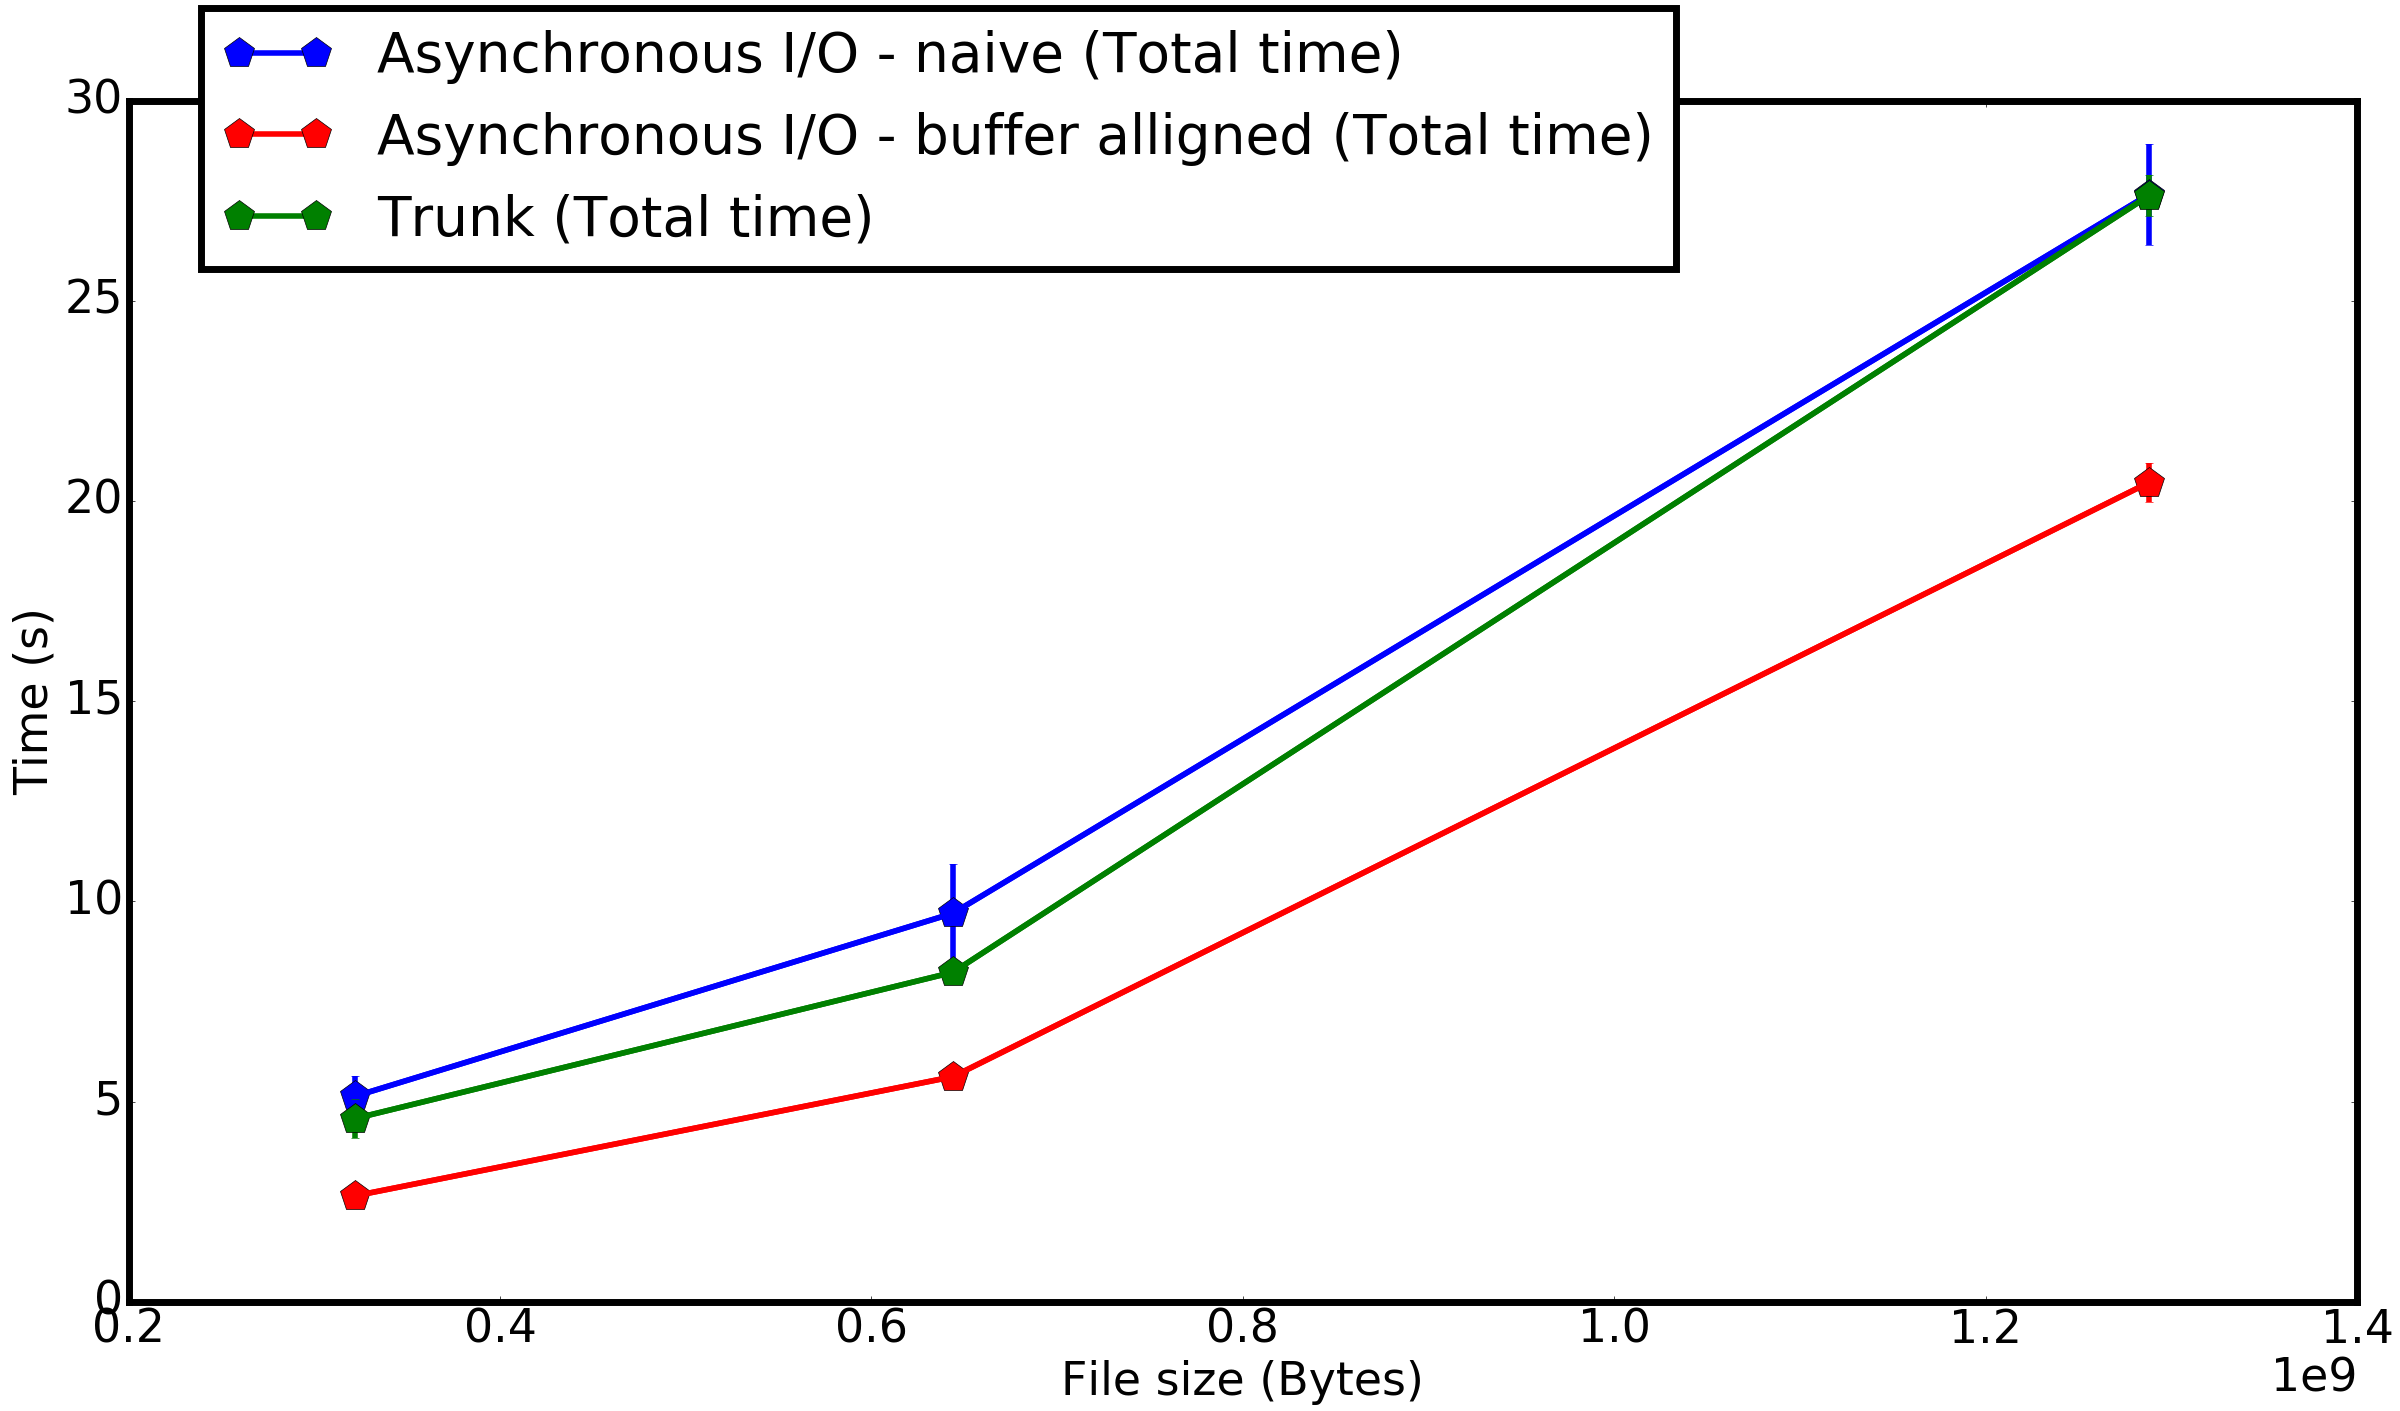
\includegraphics[width=\textwidth]{charts/cubeRemapper_falseSharing_overall_time_workstation_8core.png}
					\caption[\targetPlatformLaptop \space @ \targetPlatformLaptopFrequency]
					{{\small \targetPlatformLaptop \space @ \targetPlatformLaptopFrequency}}
					\label{fig:cubeRemapper_falseSharing_overall_time_workstation_8core}
				\end{subfigure}
				\hfill
				\begin{subfigure}[b]{0.475\textwidth}  
					\centering
					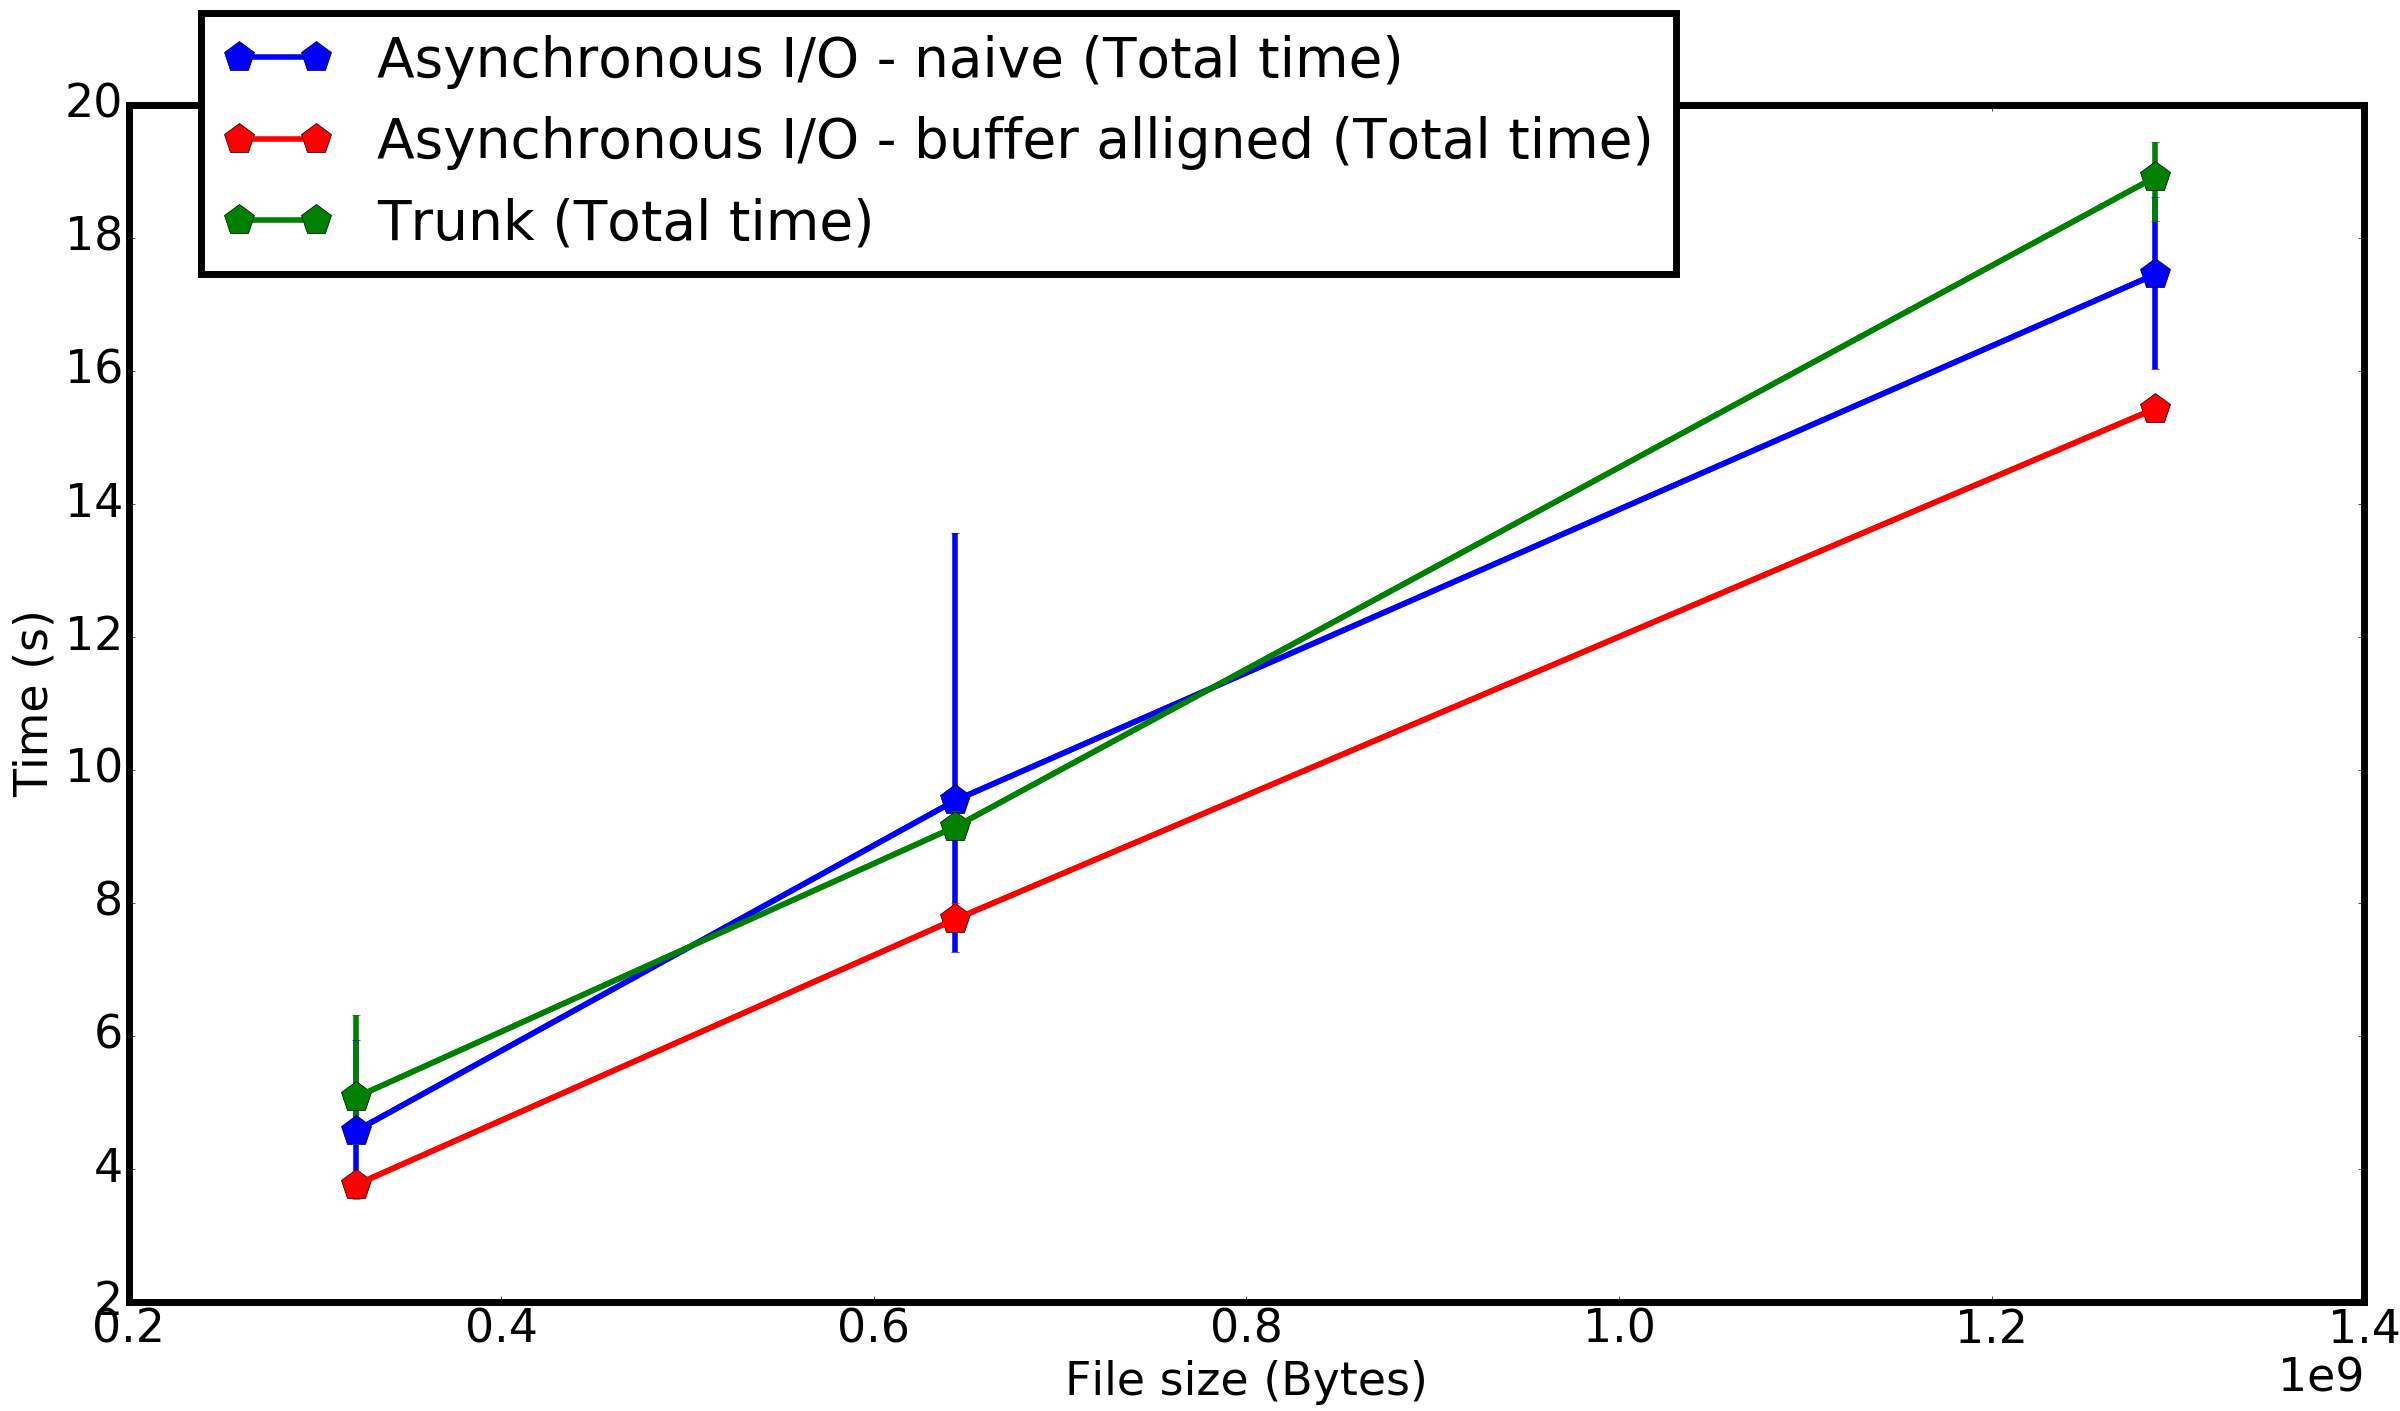
\includegraphics[width=\textwidth]{charts/cubeRemapper_falseSharing_overall_time_hpc.png}
					\caption[]%
					{{\small \targetPlatformHpc \space @ \targetPlatformHpcFrequency}}
					\label{fig:cubeRemapper_falseSharing_overall_time_hpc}
				\end{subfigure}
				\caption{Experimental comparison of the \emph{total} time: proposed \emph{\notationaio}\space (buffer aligned) VS. proposed \emph{\notationaio}\space (naive) VS. \emph{state-of-the-art} (trunk synchronous) implementation of the \toolTargetSoftware.}
				\label{fig:cubeRemapper_falseSharing_overall_time}
			\end{figure*}


	\subsection{Further improvement: adapting the dynamic memory allocation}\label{subsection:customDynamicMemAlloc}
		So far, all the performance gain has been obtained by focusing on the \emph{write} implementation.   Likewise, the improvements described in Sections \ref{subsection:improveSchedulingPolicy} and \ref{subsection:lightenFalseSharing} were aimed at reducing the perturbation of our \emph{write} implementation with respect to the \emph{compute} one.   The objective was to bring the performance of this \emph{compute} implementation \footnote{Unchanged through all the versions of the \toolTargetSoftware that we have presented till now} to the same level as that of the \emph{state-of-the-art} version.\\

		We now assess our full-fledged \notationaio\space implementation of the \toolTargetSoftware.   This final version consists in using the \emph{buffer aligned} version coupled with our custom memory allocator (see Section \ref{subsubsection:customDynamicMemoryAllocation_concept}).   Figure \ref{fig:cubeRemapper_customMemAlloc_overall_time}, which presents the experimental response time, shows that our full-fledged implementation has been able to provide a slight average gain of $19\%$ compared to the \emph{buffer aligned} implementation.   However, much more significant gain ($64\%$) is achieved when compared to the original \emph{state-of-the-art} implementation.

			\begin{figure*}[!h]
				\centering
				\begin{subfigure}[b]{0.475\textwidth}
					\centering
					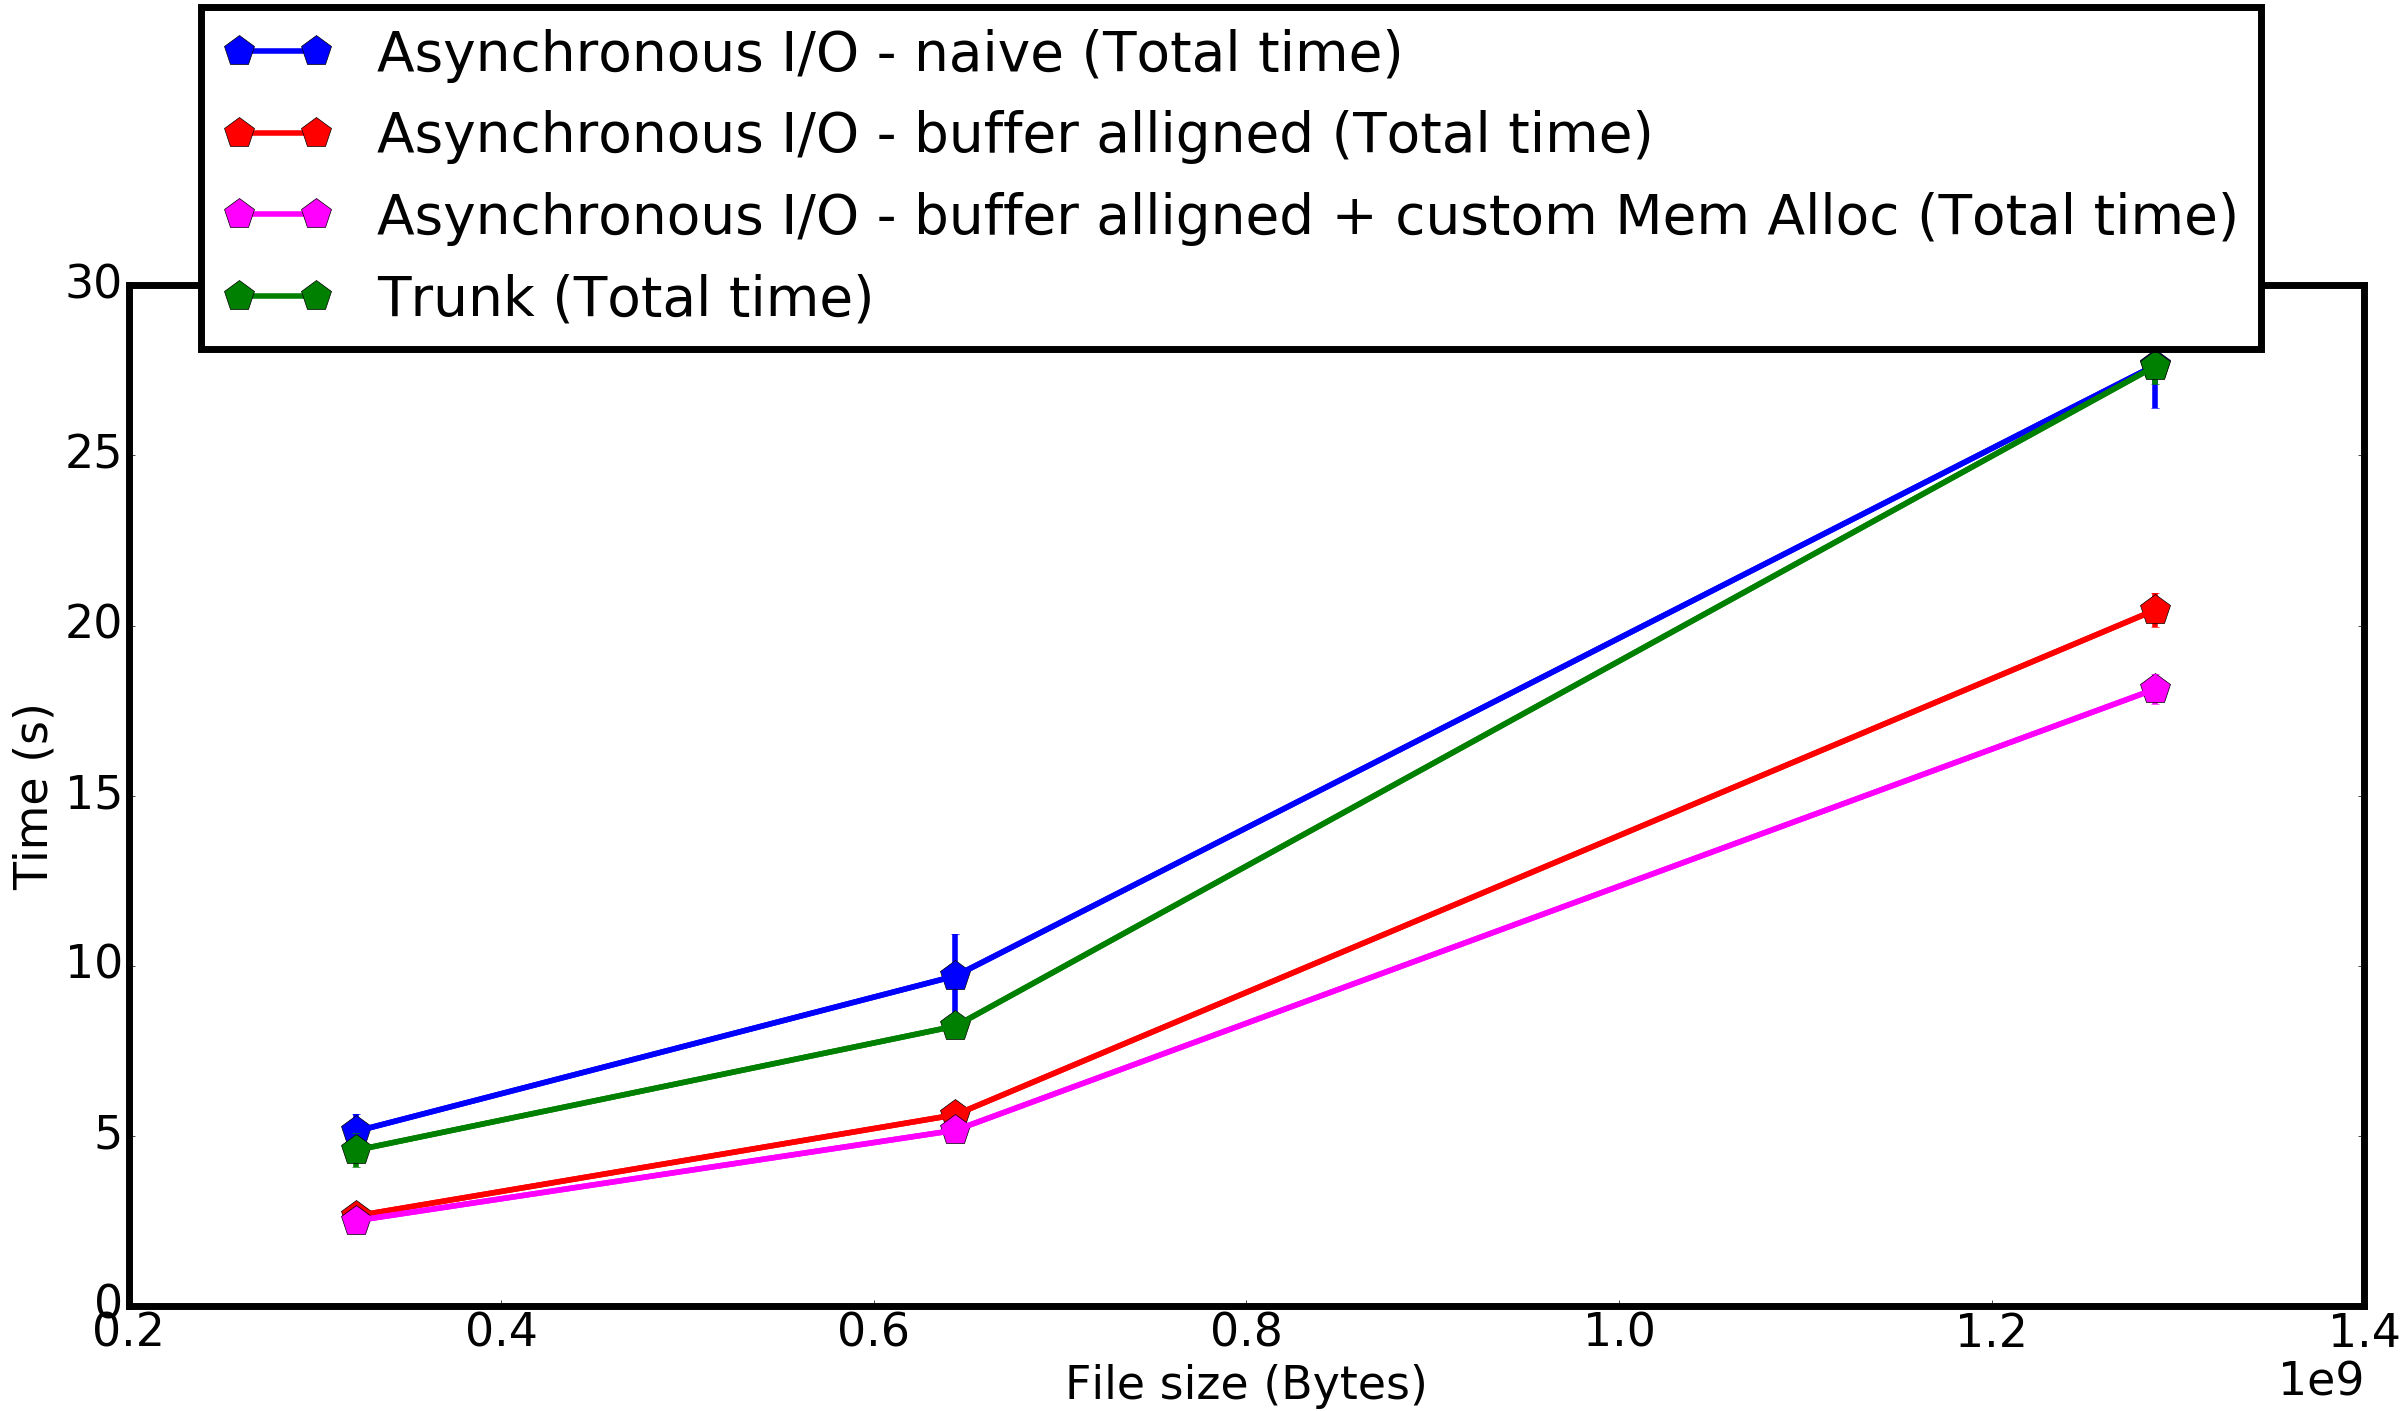
\includegraphics[width=\textwidth]{charts/cubeRemapper_customMemAlloc_overall_time_workstation_8core.png}
					\caption[\targetPlatformLaptop \space @ \targetPlatformLaptopFrequency]%
					{{\small \targetPlatformLaptop \space @ \targetPlatformLaptopFrequency}}
					\label{fig:cubeRemapper_customMemAlloc_overall_time_workstation_8core}
				\end{subfigure}
				\hfill
				\begin{subfigure}[b]{0.475\textwidth}
					\centering
					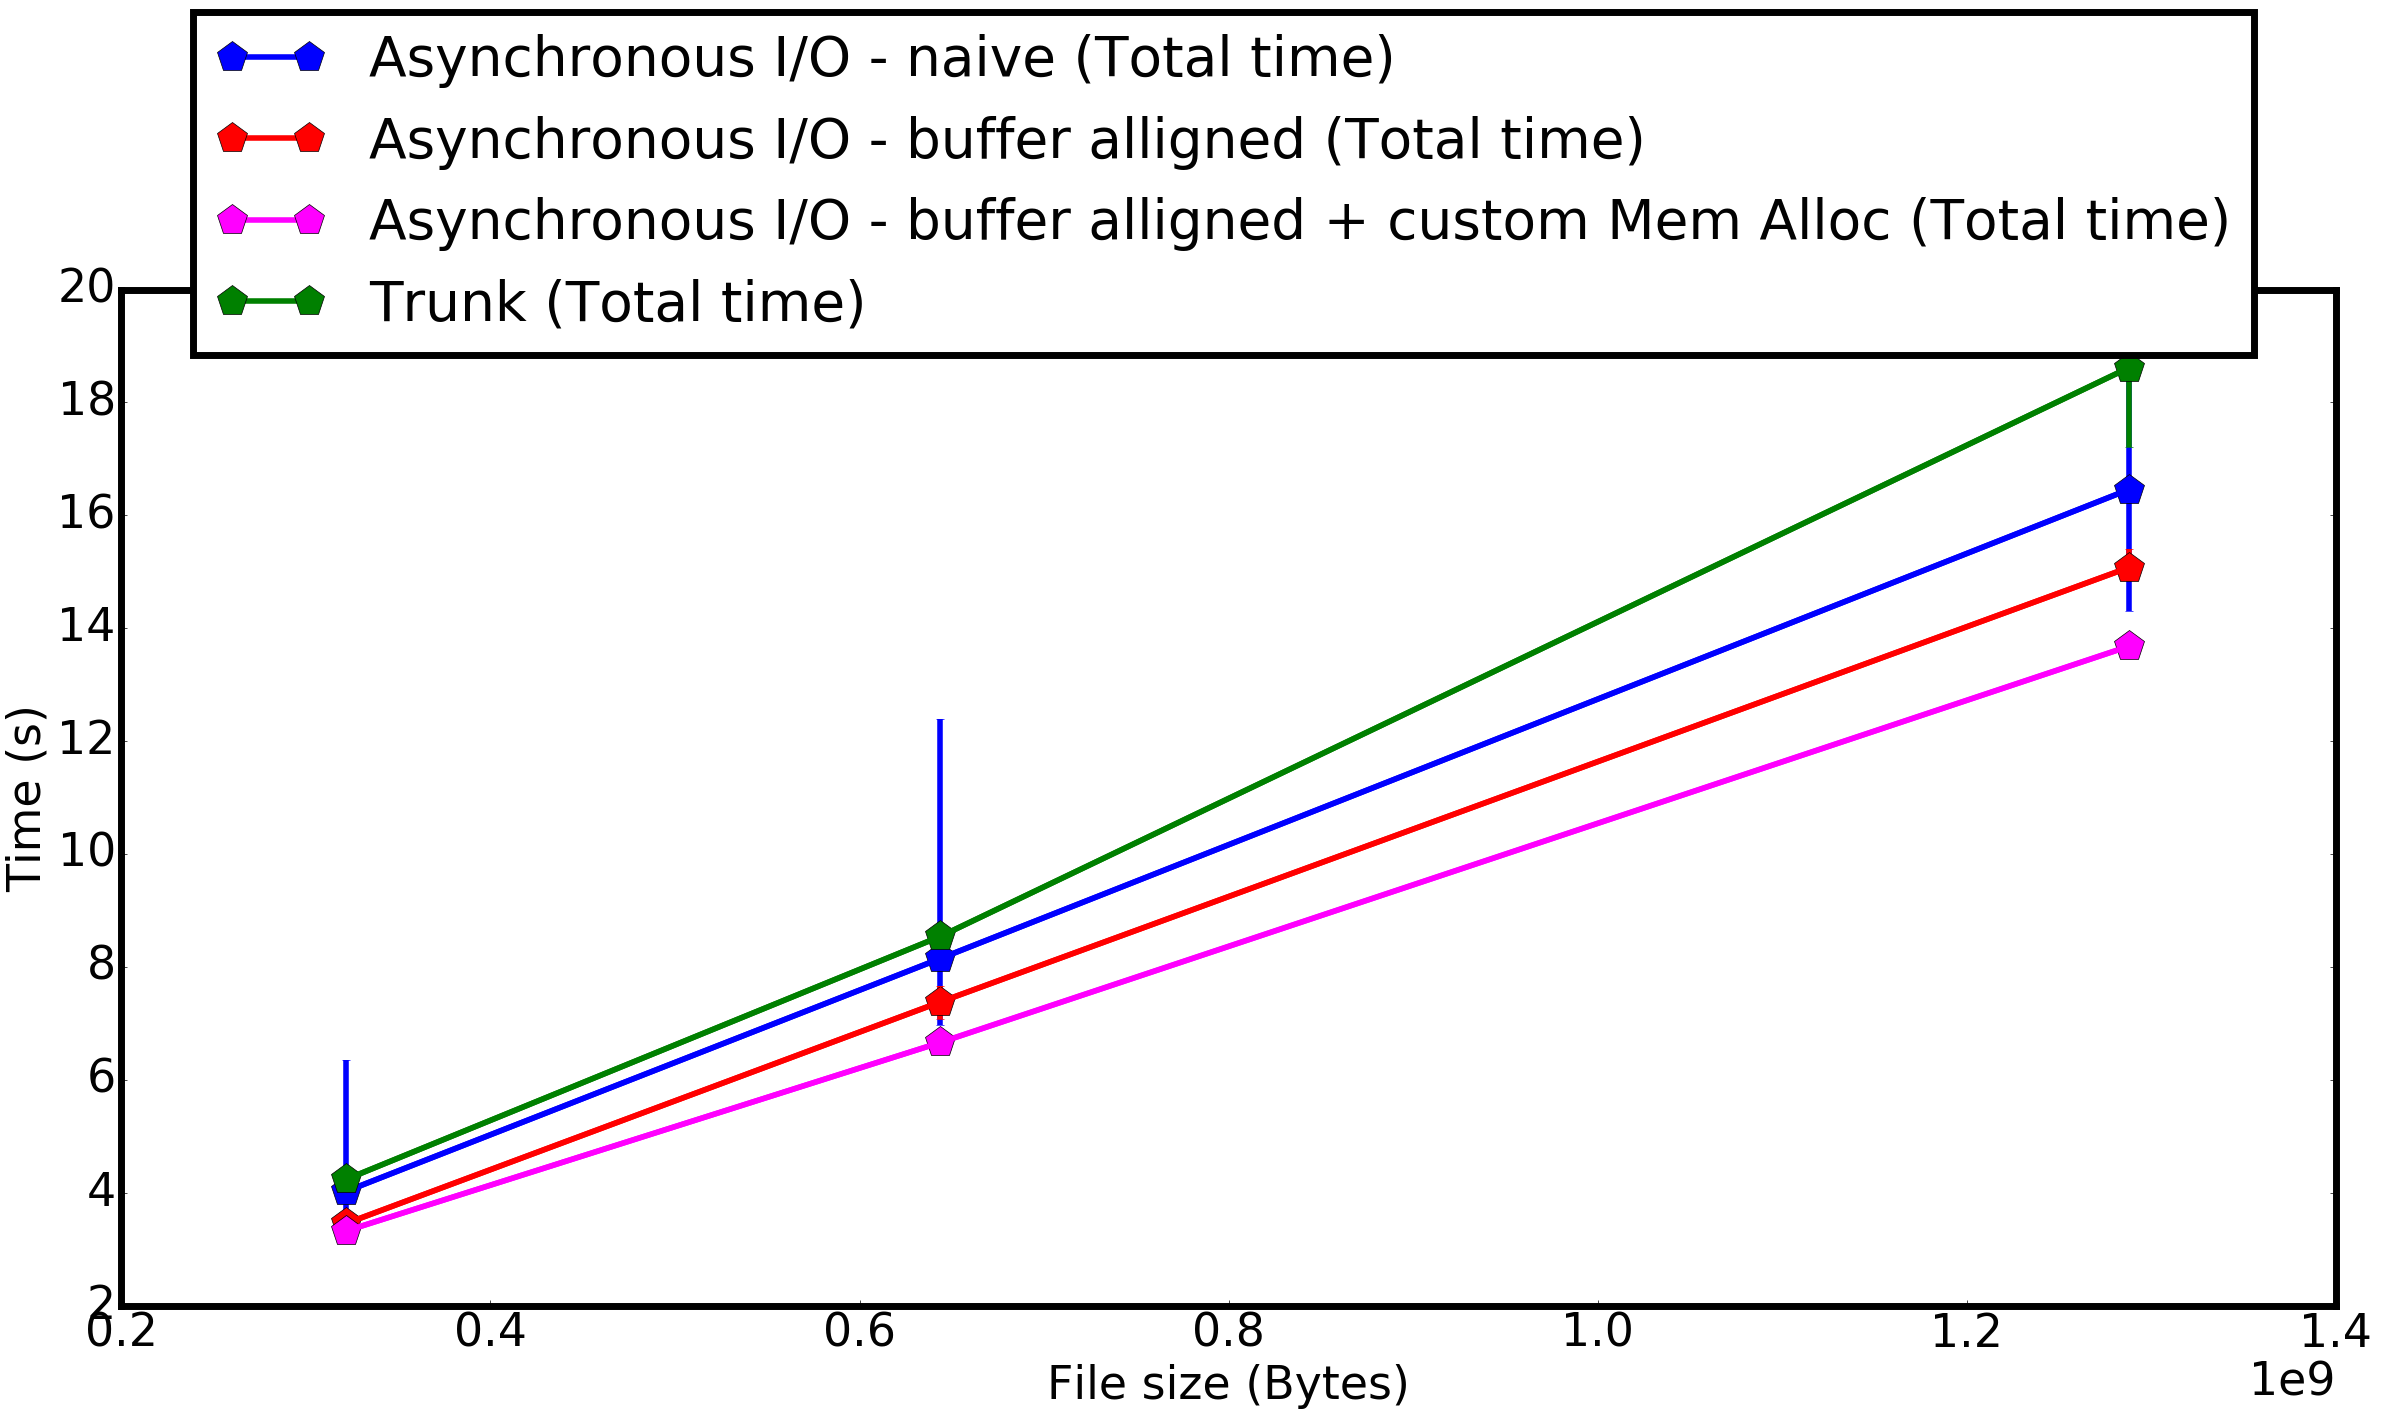
\includegraphics[width=\textwidth]{charts/cubeRemapper_customMemAlloc_overall_time_hpc.png}
					\caption[]%
					{{\small \targetPlatformHpc \space @ \targetPlatformHpcFrequency}}
					\label{fig:cubeRemapper_customMemAlloc_overall_time_hpc}
				\end{subfigure}
				\caption{Experimental comparison of the \emph{total} time: proposed \emph{full-fledged} (buffer aligned + custom mem alloc) VS. proposed \emph{\notationaio}\space (buffer aligned) VS. proposed \emph{\notationaio}\space (naive) VS. \emph{state-of-the-art} (trunk synchronous) implementation of the \toolTargetSoftware.}
				\label{fig:cubeRemapper_customMemAlloc_overall_time}
			\end{figure*}





